% EE Thesis/Dissertation
%DIF LATEXDIFF DIFFERENCE FILE
%DIF DEL first-revision/dissertation.tex   Tue Jul  2 17:22:05 2013
%DIF ADD dissertation.tex                  Tue Apr 30 16:19:55 2013
% Please see http://ee.tamu.edu/~tex for information about EE Thesis.

\documentclass[a4paper]{aitthesis}

\usepackage{graphicx}
\usepackage{latexsym}
\usepackage{amssymb,amsthm,amsmath}
%\usepackage{longtable,booktabs}
\usepackage[notocbib]{apacite}
\usepackage{verbatim}
\usepackage{multirow}
\usepackage{bm}
\usepackage{url}
\usepackage{algorithm}
\usepackage{algorithmic}
\usepackage{cancel}
\usepackage{placeins}
\usepackage{times}
\usepackage{array}
\usepackage[caption=false,font=footnotesize]{subfig}

%\usepackage{rotating}

%\usepackage{setspace}
%\singlespacing

%\setstretch{1}

%%%%%%%%%%%
% Process only the files in backets. ie title page and chapter 1 {title, ch1}
%     Be sure to remove the % before \includeonly to use this feature.

%\includeonly{title,ch1}

%%%%%%%%%%%
% Type of document.
% Keep only one of the next four lines.

%\renewcommand{\type}{Dissertation Proposal}
%\renewcommand{\type}{Dissertation}
%\renewcommand{\type}{Thesis Proposal}
%\renewcommand{\type}{Thesis}

%%%%%%%%%%%
% Type of degree.
% Keep only one of the next two lines.

%\renewcommand{\degree}{Doctor of Engineering}  % For dissertation
%\renewcommand{\degree}{Master of Engineering}   % For thesis

%%%%%%%%%%%
% Department
% Change the department if not in ELEN

%\renewcommand{\major}{Electrical Engineering}  % Change if you are not in ELEN

\newcommand{\oops}[1]{\bf{#1}}
\newcommand{\ga}{\bar{\gamma}}
\newcommand{\myint}{\int_0^{\infty}}
\renewcommand{\vec}[1]{\mathbf{#1}}
\newcommand{\mat}[1]{\mathrm{#1}}

\newcommand{\vectornorm}[1]{\left|\left|#1\right|\right|}

%\renewcommand{\vec}[1]{\boldsymbol{#1}}
%\newcommand{\mat}[1]{\mathtt{#1}}
\newcommand{\ten}[1]{\mathcal{#1}}
\newcommand{\crossmat}[1]{\begin{bmatrix} #1 \end{bmatrix}_{\times}}
\newcommand{\class}[1]{{\cal C}_{#1}}
\def\Rset{\mathbb{R}}
\def\Pset{\mathbb{P}}
\DeclareMathOperator*{\argmax}{argmax}
\DeclareMathOperator*{\argmin}{argmin}
\DeclareMathOperator*{\sign}{sign}
\def\norm{\mbox{$\cal{N}$}}

\newcommand\parms{\vec{\lambda}}
\newcommand\oldparms{\parms^{\text{old}}}

\def\short{1}
%DIF PREAMBLE EXTENSION ADDED BY LATEXDIFF
%DIF UNDERLINE PREAMBLE %DIF PREAMBLE
\RequirePackage[normalem]{ulem} %DIF PREAMBLE
\RequirePackage{color}\definecolor{RED}{rgb}{1,0,0}\definecolor{BLUE}{rgb}{0,0,1} %DIF PREAMBLE
\providecommand{\DIFadd}[1]{{\protect\color{blue}\uwave{#1}}} %DIF PREAMBLE
\providecommand{\DIFdel}[1]{{\protect\color{red}\sout{#1}}}                      %DIF PREAMBLE
%DIF SAFE PREAMBLE %DIF PREAMBLE
\providecommand{\DIFaddbegin}{} %DIF PREAMBLE
\providecommand{\DIFaddend}{} %DIF PREAMBLE
\providecommand{\DIFdelbegin}{} %DIF PREAMBLE
\providecommand{\DIFdelend}{} %DIF PREAMBLE
%DIF FLOATSAFE PREAMBLE %DIF PREAMBLE
\providecommand{\DIFaddFL}[1]{\DIFadd{#1}} %DIF PREAMBLE
\providecommand{\DIFdelFL}[1]{\DIFdel{#1}} %DIF PREAMBLE
\providecommand{\DIFaddbeginFL}{} %DIF PREAMBLE
\providecommand{\DIFaddendFL}{} %DIF PREAMBLE
\providecommand{\DIFdelbeginFL}{} %DIF PREAMBLE
\providecommand{\DIFdelendFL}{} %DIF PREAMBLE
%DIF END PREAMBLE EXTENSION ADDED BY LATEXDIFF

\begin{document}

\pagenumbering{roman}
\pagestyle{plain}
%==========================================================
%======================  FRONT STUFF ======================
%==========================================================

%======================= Cover Page =======================
%\begin{document}
\newpage

\DIFdelbegin %DIFDELCMD < \pagestyle{plain}
%DIFDELCMD < \pagenumbering{roman}
%DIFDELCMD < \setcounter{page}{1}
%DIFDELCMD < %%%
\DIFdelend \DIFaddbegin 

%DIF >  Set this page style from plain to empty, so the page number 
%DIF >  will not be put on this page.
\pagestyle{empty}

%DIF > \pagenumbering{roman}
%DIF > \setcounter{page}{1}

\DIFaddend \addcontentsline{toc}{section}{Title Page}
%\setlength{\footskip}{-15mm}
\setlength{\textheight}{230mm}
\setlength{\voffset}{10mm}
\vskip -5em

\begin{center}
{ 
%DIF >     \singlespace \uppercase{\bf Incremental Behavior Modeling and
%DIF >     Suspicious Activity Detection} \par
    \singlespace \DIFdelbegin %DIFDELCMD < \uppercase{\bf Incremental Behavior Modeling and
%DIFDELCMD <     Suspicious Activity Detection} %%%
\DIFdelend \DIFaddbegin {\large \bf \DIFadd{Incremental Behavior Modeling and
    Suspicious Activity Detection}} \DIFaddend \par
}
\vskip 2em
{
    \lineskip 1.5em
    \begin{tabular}[t]{c} by\\ \\ Kan Ouivirach
    \end{tabular}\par
}
%\vskip 5.6em

\vskip 3.5em
\singlespace A dissertation submitted in partial fulfillment of the
requirements for the\\ degree of Doctor of Philosophy in\\ Computer
Science

%DIF < 	\vskip 5em
%DIF > \vskip 5em
\vskip 0.5em
{
    \singlespace
    \begin{center}
        \begin{tabular}{rl}
        \\[-1em]
        Examination Committee: & Dr.\ Matthew N.\ Dailey (Chairperson) \\[-0.8em]
                               & Dr.\ Nitin V.\ Afzulpurkar \\[-0.8em]
                               & Dr.\ Supavadee Aramvith \DIFaddbegin \DIFadd{(External Expert) }\DIFaddend \\[-0.8em]
                               & Dr.\ Sanparith Marukatat \DIFaddbegin \DIFadd{(External Expert) }\DIFaddend \\\\

        External Examiner:     & Prof.\ James J.\ Clark \\[-0.8em]
                               & Dept.\ of Electrical and Computer Engineering \\[-0.8em]
                               & McGill University, Canada \\\\

        Nationality:     & Thai \\[-0.8em]
        Previous Degree: & Master of Engineering in Computer Science\\[-0.8em]
                         & Asian Institute of Technology, Thailand\\[-0.8em]
        \\
        Scholarship Donor: & Royal Thai Government \DIFaddbegin \DIFadd{Fellowship }\DIFaddend \\[-0.8em]
        \\
        \end{tabular}
    \end{center}

    \vskip 3.0em
    \centerline{}
    \vskip 2em
}
\end{center}
\begin{center}
    \singlespace Asian Institute of Technology\\ School of Engineering
                  and Technology\\ Thailand\\ \DIFdelbegin \DIFdel{May }\DIFdelend \DIFaddbegin \DIFadd{December }\DIFaddend 2013
\end{center}
\vfill

%====================== ACKNOWLEDGEMENTS ======================
\newpage

\DIFaddbegin 

\DIFaddend \pagestyle{plain}

\DIFaddbegin 

%DIF >  Maybe these two commands below are not necessary.
\pagenumbering{roman}
\setcounter{page}{2}

\DIFaddend \addcontentsline{toc}{section}{Acknowledgments}
\onecolumn % Single-column.
\if@twoside\else\raggedbottom\fi % Ragged bottom unless twoside option.
\setlength{\footskip}{8mm}
\begin{center}
{
    \large \bf Acknowledgments\\ \vskip 1em
}
\vskip 1em
\end{center}
\singlespace
\doublespace
\hspace{8.5mm}
\vspace{-1em}

My research work was accomplished through the support of many
people. I would like to thank all of them here.

First, my deepest thanks and a special word of appreciation go to 
my beloved parents, who always inspire and give me endless unconditional 
love and support. I dedicate this piece of work to them.

Second, I would like to express my sincere thanks to my advisor, 
Dr.\ Matthew N.\ Dailey, for giving me invaluable advice, excellent 
guidance, strong encouragement and support throughout the study with his
kindness and cordial attitude. I also thank him for being very patient
with me and always willingly answering all my questions.

Third, I would like to extend my sincere gratitude to my committee 
members, Dr.\ Nitin V.\ Afzulpurkar, Dr.\ Supavadee Aramvith, 
and Dr.\ Sanparith Marukatat, for their valuable suggestions
and constructive criticism.

Fourth, I would like to thank the Royal Thai Government for their 
graduate scholarship throughout my studies at AIT. Without the 
scholarship, studying at AIT would be impossible.

\DIFaddbegin \DIFadd{Fifth, I would like to thank Prof.}\ \DIFadd{James J.}\ \DIFadd{Clark for the careful 
review and constructive comments. 

}

\DIFaddend Finally, I am very grateful to have been a part of the AIT Vision and 
Graphics Lab (VGL). I am thankful to all of the lab members for 
valuable discussions and comments on this work. Special thanks are 
due to Shashi Gharti, who assisted with the implementation of human 
tracking and feature extraction, and Phattanapon Rhienmora, who has 
been encouraging and supporting me during my Ph.D.\ life.

%====================== PUBLICATIONS ======================


%====================== ABSTRACT ======================
\newpage
\pagestyle{plain}
\addcontentsline{toc}{section}{Abstract}
\onecolumn % Single-column.
\if@twoside\else\raggedbottom\fi % Ragged bottom unless twoside option.

\setlength{\footskip}{8mm}

\begin{center}
{\large \bf Abstract \\ \vskip 1em}
\vskip 1em
\end{center}
\singlespace
\doublespace
\hspace{8.5mm}
\vspace{-1em}

Video surveillance systems have become widespread tools for monitoring
and law enforcement in public areas.  Due to increasing crime, video
surveillance systems are being deployed in more and more places.
Video surveillance systems are needed to help security personnel
prevent and respond to criminal activity in a timely fashion.
However, human monitoring becomes increasingly expensive and
ineffective as the amount of video data increases. Also, manual review of
all video footage is time-intensive and error-prone.

Automated anomaly detection can help to improve the effectiveness of
human observers by separating the video stream into a sequence of
``normal'' and ``unusual'' events. However, much of the existing work
has many limitations in this direction. Oftentimes, separate models
for each distinct a priori known class of ``normal'' behavior are
assumed.  This could lead to the problem of typical behavior evolving
and becoming more diverse to the point that the false alarm rates
increase.  The naive solution would be to retain all of the
observation data and retrain the system periodically, but this
requires storing all of the incoming data, requiring too much disk
space. In this dissertation, we therefore propose and evaluate an
efficient method for incremental automatic identification of
suspicious behavior in video surveillance data.

First, we develop a blob extraction method that segments blobs and an
appearance-based blob tracking method that uses a forward-backward
overlap method and color coherence vectors (CCVs) to maintain identity
through blob merging and splitting cases.

Second, we propose a new method for detecting shadows using a simple
maximum likelihood formulation based on HSV color information. We find
that the method outperforms standard shadow detection methods on three
different real-world video surveillance data sets.

Third, we propose a new method for clustering human behaviors in the
context of video surveillance that is suitable for bootstrapping an
anomaly detection module for intelligent video surveillance
systems. We show that the method is extremely effective in separating
anomalous from typical behaviors on real-world testbed video
surveillance data.

Fourth, we propose a \textit{semi-supervised} batch anomaly
detection method that self-calibrates itself from a small bootstrap
set in which each bootstrap sequence is manually labeled as normal or
suspicious by a human operator. Our method proves extremely effective,
with a very low false alarm rate at a 100\% hit rate.

Finally, we propose an effective behavior modeling and suspicious
activity detection method extending the batch method that
incrementally learns scene-specific statistical models of human
behavior without requiring storage of historical data. The incremental
method's false alarm rate drops below that of the batch method on the
same data.

In experimental evaluations on real-world testbed video surveillance
data sets, the proposed methods prove to be practical and effective at
inducing scene-specific statistical models useful for bringing
suspicious behavior to the attention of human security personnel.

\setlength{\parskip}{0pt} 
%======================= Table of Contents =========================
\newpage
\addcontentsline{toc}{section}{Table of Contents}
\tableofcontents

% Page 2 begins

%===================== List of Figures ======================
\newpage
\addcontentsline{toc}{section}{List of Figures}
\listoffigures

%\clearpage     % \clearpage ends the page, and also dumps out all floats.
%\end{document} % Floats are things like tables and figures.

%\clearpage     % \clearpage ends the page, and also dumps out all floats.

% %===================== List of Tables ======================
\newpage
\addcontentsline{toc}{section}{List of Tables}
\listoftables

% %\clearpage     % \clearpage ends the page, and also dumps out all floats.
% %\end{document} % Floats are things like tables and figures.

%\clearpage     % \clearpage ends the page, and also dumps out all floats.

% %===================== List of Symbols ======================
\newpage
\addcontentsline{toc}{section}{List of Symbols}

\begin{center}
    {\large \bf List of Symbols\\ \vskip 1em}
    \vskip 1em
\end{center}
\singlespace

\begin{table}[h]
    \begin{tabular}{lll}
        \DIFdelbeginFL \DIFdelFL{Test }\DIFdelendFL \DIFaddbeginFL \DIFaddFL{$\vec{f}_i^t$ }\DIFaddendFL & & \DIFdelbeginFL \DIFdelFL{This is a test}\DIFdelendFL \DIFaddbeginFL \DIFaddFL{Feature vector of track $i$ at time $t$}\DIFaddendFL . \\
        \DIFdelbeginFL \DIFdelFL{What }\DIFdelendFL \DIFaddbeginFL \DIFaddFL{$V$ }\DIFaddendFL & & \DIFdelbeginFL \DIFdelFL{This is a what. }\DIFdelendFL \DIFaddbeginFL \DIFaddFL{Set of discrete categories (cluster IDs). }\\
        \DIFaddFL{$U$ }& & \DIFaddFL{Number of categories.  }\\
        \DIFaddFL{$\Theta$ }& & \DIFaddFL{Model estimate for shadows. }\\ 
        \DIFaddFL{$sh$ }& & \DIFaddFL{Shadow. }\\
        \DIFaddFL{$obj$ }& & \DIFaddFL{Object. }\\
        \DIFaddFL{$L_i$ }& & \DIFaddFL{Log of the probability of a sequence $O_i$ given the HMM $M_c$. }\\
        \DIFaddFL{$\vec{O_i}$ }& & \DIFaddFL{Observation sequence $i$. }\\
        \DIFaddFL{$T_i$ }& & \DIFaddFL{Number of observations in sequence $i$. }\\
        \DIFaddFL{$M_c$ }& & \DIFaddFL{HMM that models the sequences in cluster $c$. }\\
        \DIFaddFL{$p_c$ }& & \DIFaddFL{Optimal rejection threshold for cluster $c$. }\\
        \DIFaddFL{$N_c$ }& & \DIFaddFL{Number of deviant patterns allowed in cluster $c$. }\\
        \DIFaddFL{$z$ }& & \DIFaddFL{$z$-value. }\\
        \DIFaddFL{$\theta_z$ }& & \DIFaddFL{Global alarm threshold. }\\

        
    \DIFaddendFL \end{tabular}
\end{table}

% %===================== List of Acronyms ======================
\newpage
\addcontentsline{toc}{section}{List of Acronyms}

\begin{center}
    {\large \bf List of Acronyms\\ \vskip 1em}
    \vskip 1em
\end{center}

\singlespace

\begin{table}[h]
    \begin{tabular}{lll}
        \DIFaddbeginFL \DIFaddFL{CCTV   }& & \DIFaddFL{Closed-Circuit Television. }\\
        \DIFaddFL{MoG    }& & \DIFaddFL{Mixture of Gaussian. }\\
        \DIFaddFL{CCV    }& & \DIFaddFL{Color Coherence Vector. }\\
        \DIFaddFL{DNM    }& & \DIFaddFL{Deterministic Nonmodel-Based. }\\
        \DIFaddFL{NCC    }& & \DIFaddFL{Normalized Cross-Correlation. }\\
        \DIFaddFL{ML     }& & \DIFaddFL{Maximum Likelihood. }\\
        \DIFaddFL{IML    }& & \DIFaddFL{Incremental Maximum Likelihood. }\\
        \DIFaddFL{EM     }& & \DIFaddFL{Expectation Maximization. }\\  
        \DIFaddFL{DBN    }& & \DIFaddFL{Dynamic Bayesian Network. }\\
        \DIFaddFL{$k$-NN }& & \DIFaddFL{$k$-Nearest Neighbors. }\\
        \DIFaddFL{SVM    }& & \DIFaddFL{Support Vector Machine. }\\
        \DIFaddFL{PCA    }& & \DIFaddFL{Principal Component Analysis. }\\
        \DIFaddFL{MDL    }& & \DIFaddFL{Minimum Description Length. }\\
        \DIFaddFL{GMM    }& & \DIFaddFL{Gaussian Mixture Model. }\\
        \DIFaddendFL HMM    & & Hidden Markov Model. \\
        DTW    & & Dynamic Time Warping. \\ 
        \DIFaddbeginFL \DIFaddFL{LRT    }& & \DIFaddFL{Likelihood Ratio Test. }\\
        \DIFaddendFL ROC    & & Receiver Operating Characteristic. \\
        \DIFaddbeginFL \DIFaddFL{EER    }& & \DIFaddFL{Equal Error Rate.
    }\end{tabular}
\end{table}

\newpage

\begin{table}[h]
    \begin{tabular}{lll}
        \DIFaddendFL TP     & & The number of True Positive. \\ 
        FP     & & The number of False Positive. \\
        TN     & & The number of True Negative. \\ 
        FN     & & The number of False Negative. \\
        TPR    & & True Positive Rate. \\ 
        FPR    & & False Positive Rate. 
    \end{tabular}
\end{table}

\setlength{\parskip}{12pt}


\small

\pagenumbering{arabic}
\setlength{\headheight}{12pt}
\pagestyle{plain}

% uncomment the line below for the final version
%\topmargin -3cm

\setlength{\footskip}{8mm}

\chapter{Introduction} 

\textit{This dissertation explores the possibilities and develops
algorithms for modeling human behaviors and detecting anomalies
without requiring large databases of training data. In this chapter, I
discuss the background \DIFaddbegin \DIFadd{of, }\DIFaddend and motivation \DIFdelbegin \DIFdel{of }\DIFdelend \DIFaddbegin \DIFadd{for }\DIFaddend my work\DIFaddbegin \DIFadd{. Additionally}\DIFaddend , 
\DIFaddbegin \DIFadd{I }\DIFaddend review real-world surveillance systems, present the contributions of 
the work, and provide an outline of this dissertation.}

\section{Background and Motivation}

Due to the increase in demand for video surveillance in public areas,
video surveillance is becoming ubiquitous in our lives. It becomes
increasingly important for preventing and responding to \DIFdelbegin \DIFdel{terrorist }\DIFdelend \DIFaddbegin \DIFadd{terroristic 
threats }\DIFaddend and other criminal activities. However, the resulting proliferation of
surveillance cameras is making it increasingly difficult to monitor
all channels continuously. Human monitoring is therefore becoming
increasingly expensive and ineffective as the torrent of video data
increases. For instance, in a CCTV monitoring room (see
Figure \ref{fig:monitoring}), security operators are required to
monitor 24 hours a day and be ready to take action when an alarm
occurs. Security will be enhanced if there is an intelligent
surveillance system able to perform filtering, \DIFdelbegin \DIFdel{archiving }\DIFdelend \DIFaddbegin \DIFadd{archive }\DIFaddend ``normal''
events, and automatically \DIFdelbegin \DIFdel{raising }\DIFdelend \DIFaddbegin \DIFadd{raise }\DIFaddend alarms for possible ``abnormal''
events or presenting such events to human security personnel for
consideration as a security threat. The problems to consider in a
surveillance system include pedestrian detection and tracking,
unattended object detection, human behavior modeling, and anomaly
detection.

\begin{figure}[t]
    \centering
    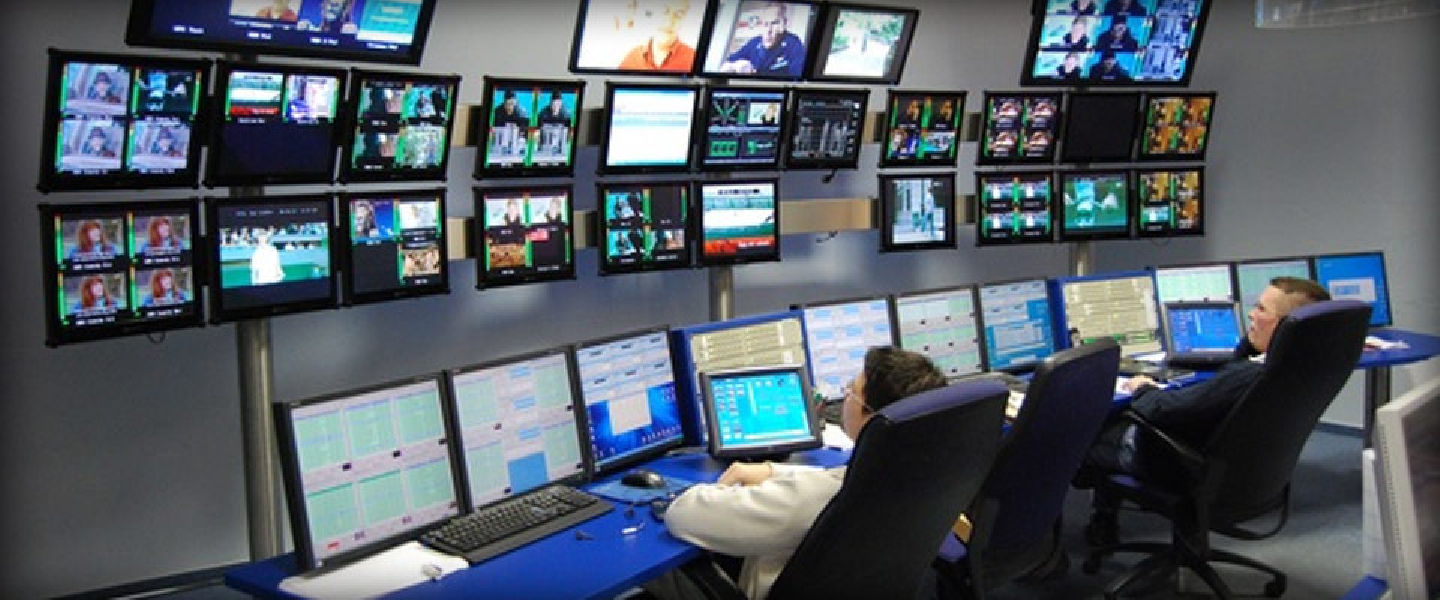
\includegraphics[width=5in]{figures/monitoring}
    \caption[CCTV monitoring room.]{\small CCTV monitoring
        room. Reprinted from the Twenty First Security Web site
        (\url{http://www.twentyfirstsecurity.com.au/}).}
    \label{fig:monitoring}
\end{figure}

Human behavior understanding is one of the \DIFdelbegin \DIFdel{key components }\DIFdelend \DIFaddbegin \DIFadd{most intricate and complex facets }\DIFaddend of
intelligent video surveillance. 
\DIFdelbegin \DIFdel{However, the }\DIFdelend \DIFaddbegin \DIFadd{Clearly, behavioral understanding can be problematic because it requires 
considerable time to study each individual subject, and often cannot 
predict ``one-time'' malicious behavior before it happens.
The }\DIFaddend problem is difficult and
remains unsolved, due to the wide range of activities possible in any
given context and the large amount of variability within any
particular activity.

One limitation of much of the existing work is that it learns in batch
mode and creates separate models, which remain static once trained,
for each distinct class of behavior. It may have an advantage in
explaining data that are well-defined, but it needs sufficiently large
samples of behavior patterns before training the system. Another
limitation is that the number of ``normal'' behavior patterns needs to
be known beforehand because we cannot learn a model for ``abnormal''
behavior that is rare and diverse. Therefore, we must instead detect
deviations from typical behavior.

The ambiguity of human behaviors makes the problem more challenging
since it is scene-dependent and can change over time. In particular, a
behavior considered normal in one context might be considered unusual
in another context depending on the type of behavior and where and
when it is observed. The characteristics of typical behavior also vary
from scene to scene.

Many researchers have attempted to build surveillance systems able to
interpret and understand human behaviors. However, most of the work
learns behaviors in an offline fashion and keeps the model static once
trained. This is impractical for real-time surveillance applications,
since offline training requires a great deal of computational time and
resources. In addition, the number of behaviors needs to be known
beforehand. We therefore need to find a way to initially recognize and
model each of the common behavior groups in a particular scene as well
as to incrementally learn scene-specific models as new behavior is
observed.

Many open source and commercial video surveillance products are 
available. Most of the products do not implement any intelligent
features; therefore, they cannot learn and understand the events
occurring in a scene. Moreover, a great deal of configuration must be done
before a user can deploy the system to operate in a real situation.
For instance, a user may need to define restricted zones or rules
for a specific scene.

Three main challenges for human behavior understanding and anomaly
detection are as follows.

\begin{enumerate}
    \item It is impractical to store all data in a system; therefore, we
        need an efficient approach that learns scene-specific statistical
        models of human behavior without requiring storage of large
        databases of training data.
    \item Real human behavior is sometimes ambiguous; therefore, we need to 
        keep humans such as security personnel in the loop to interpret it.
    \item Unusual behavior is rare and diverse, and it is also impractical 
        to acquire sufficient data for a good model for it; therefore, we 
        need to detect deviations from typical behavior instead.
\end{enumerate}

In this dissertation, we propose to explore, implement, and evaluate
an efficient method for automatic identification of suspicious
behavior in video surveillance data that incrementally learns
scene-specific statistical models of human behavior without requiring
storage of large databases of training data. The method is based on
hidden Markov models (HMMs) with sufficient statistics and an optimal
threshold on the likelihood of an event according to the human
behavior model.  We begin by building an initial set of models
explaining the behaviors occurring in a small bootstrap data set. The
bootstrap procedure partitions the bootstrap set into clusters then
assigns new observation sequences to clusters based on statistical
tests of HMM log likelihood scores. Cluster-specific likelihood
thresholds are learned rather than set arbitrarily. After
bootstrapping, each new sequence is used to incrementally update the
sufficient statistics of the HMM it is assigned to. Our method is an
effective solution to the problem of inducing scene-specific
statistical models useful for bringing suspicious behavior to the
attention of human security personnel.

\section{Review of \DIFdelbegin \DIFdel{Real-World }\DIFdelend \DIFaddbegin \DIFadd{State of the Art in }\DIFaddend Surveillance Systems}

We divide this section into \DIFaddbegin \DIFadd{two parts. The first part describes the 
review of }\DIFaddend open source and commercial products. \DIFaddbegin \DIFadd{The second part describes 
the review of the state of the art in surveillance systems.

}\DIFaddend 

\subsection{Open Source \DIFaddbegin \DIFadd{and Commercial }\DIFaddend Products}

ZoneMinder (ZM; Coombes, 2007)\nocite{zoneminder} is an open source
video surveillance system for Linux. It has been released under the
terms of the GNU general public license (GPL). ZM supports both IP
cameras and USB cameras. Figure \ref{fig:zm-webcam} shows an example
of a scene captured by an IP camera and a USB camera. The system
consists of many independent modules including motion detection.  Each
component is designed to use as few resources as possible, maximizing
the efficiency of the machine. It provides a PHP-based Web interface
that allows us to control the cameras and monitor a scene from
anywhere. Besides controlling and monitoring, we can also review,
archive, or delete the events through its Web interface.

\begin{figure}[t]
  \begin{center}
    \subfloat[]{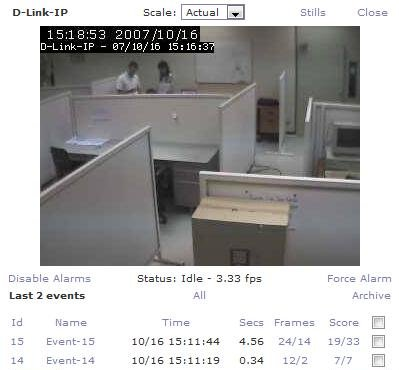
\includegraphics[scale=0.6]{figures/zm-webcam01.jpg}
    \label{fig:zm-webcam01}}
    \hspace{0.1in}
    \subfloat[]{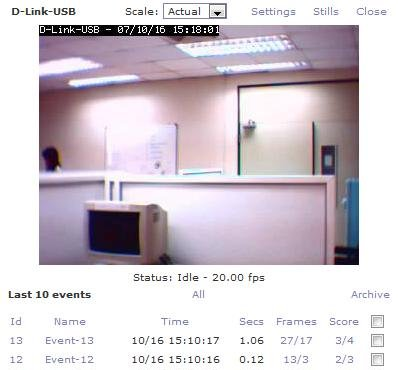
\includegraphics[scale=0.6]{figures/zm-webcam02.jpg}
    \label{fig:zm-webcam02}}
  \end{center}
  \caption[Example of a scene captured by ZoneMinder.]{\small Example
    of a scene captured by (a) an IP camera and (b) a USB camera from
    ZoneMinder.}
  \label{fig:zm-webcam}
\end{figure}

SecureCam \shortcite{bedecs09securecam} is \DIFdelbegin \DIFdel{a }\DIFdelend \DIFaddbegin \DIFadd{an }\DIFaddend open source software
\DIFdelbegin \DIFdel{for
}\DIFdelend \DIFaddbegin \DIFadd{project for the }\DIFaddend Windows platform providing a friendly user interface as
shown in Figure \ref{fig:securecam}. Similar to ZoneMinder, SecureCame
supports multiple cameras and provides a few simple and fast
algorithms such as motion detection. It has e-mail and sound
notification features, and it also allows users to record video for
later review.

\begin{figure}[t]
  \begin{center}
    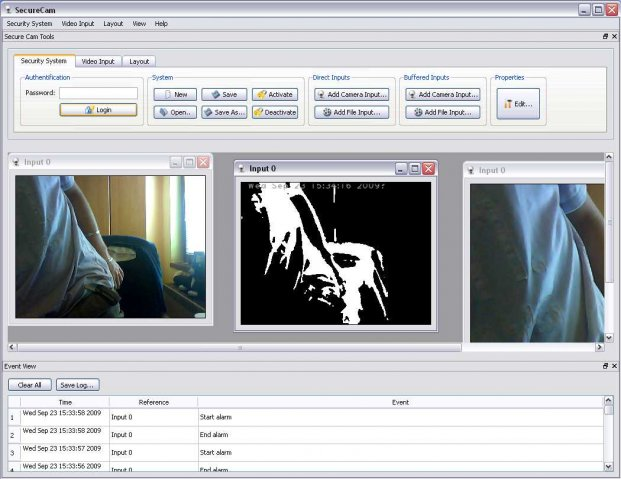
\includegraphics[width=4in]{figures/securecam.jpg}
    \caption[Screen shot of SecureCam.]{\small Screen shot of
      SecureCam. Reprinted from the SecureCam Web site
      (\url{http://sourceforge.net/projects/securecam/}).}
    \label{fig:securecam}
  \end{center}
\end{figure}

\DIFdelbegin \subsection{\DIFdel{Commercial Products}}

%DIFAUXCMD
\addtocounter{subsection}{-1}%DIFAUXCMD
%DIFDELCMD < 

%DIFDELCMD < %%%
\DIFdelend Vitamin D Video \shortcite{vitamind} is a commercial video
surveillance system. It supports USB webcams and network cameras and
provides advanced features such as creating rules for specific events.
For example, the user could create a rule to record a clip only when a
person opens \DIFdelbegin \DIFdel{the }\DIFdelend \DIFaddbegin \DIFadd{a }\DIFaddend door, or the user could create a rule to notify via
email when the system senses some movement in a defined region. The
system also allows users to monitor a scene and to search for videos
of interest.  Figure \ref{fig:vitamind} shows a screen shot of the
software.

\begin{figure}[t]
  \begin{center}
    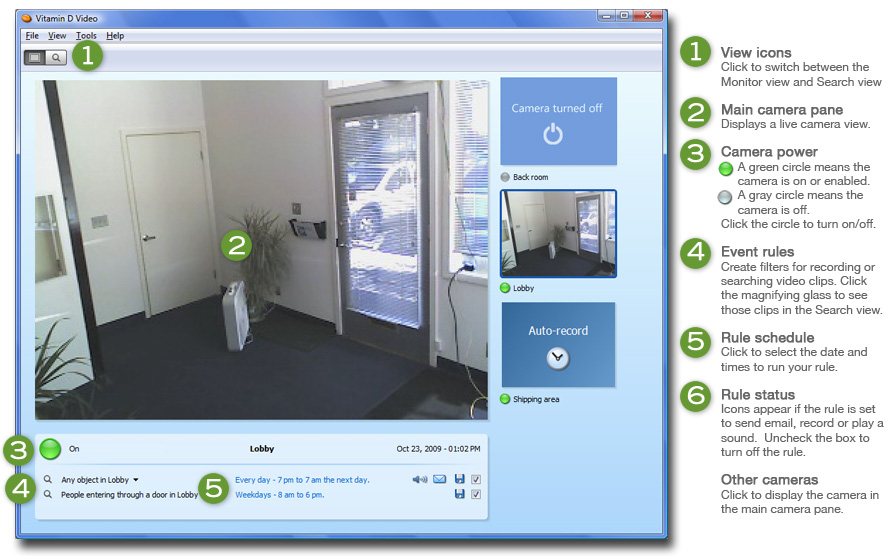
\includegraphics[width=4in]{figures/vitamind.jpg}
    \caption[Screen shot of Vitamin D Video.]{\small Screen shot of
      Vitamin D Video. Reprinted from the Vitamin D Video Web site
      (\url{http://www.vitamindinc.com/}).}
    \label{fig:vitamind}
  \end{center}
\end{figure}

It is interesting that Vitamin D Video does not use motion detection,
but rather uses people detection. It uses hierarchical temporal memory
(HTM; Hawkins, 2007)\nocite{jeff07htm} to detect people. This
algorithm attempts to apply the concept of how the brain recognizes a
\DIFdelbegin \DIFdel{person}\DIFdelend \DIFaddbegin \DIFadd{human being}\DIFaddend .

Video Analytics \shortcite{dvtel} is a video surveillance software
package that includes many different modules.  Sample modules are
intrusion detection, unattended baggage detection, object removal
detection, autonomous pan-tilt-zoom (PTZ) tracking, stopped vehicle
detection, loitering detection, and camera tampering
detection. However, some modules such as intrusion detection do not
have any intelligent features.

SuperTrack \shortcite{supertrack} is an intelligent video surveillance
system. SuperTrack is designed for automatically analyzing and
monitoring events without the need for human attention and
interaction. This system provides automatic object detection, abnormal
behavior detection, tracking, and so on. However, it requires the user
to configure and maintain a set of alarm trigger rules in
advance. SuperTrack also supports various types of cameras such as USB
cameras and network cameras.  Figure \ref{fig:supertrack} shows a
screen shot of the system.

\begin{figure}[t]
  \begin{center}
    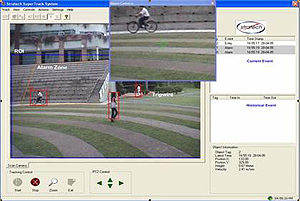
\includegraphics[width=3in]{figures/supertrack.jpg}
    \caption[Screen shot of SuperTrack.]{\small Screen shot of
      SuperTrack. Reprinted from the Stratech Web site
      (\url{http://www.stratechsystems.com/iv_supertrack.asp}).}
    \label{fig:supertrack}
  \end{center}
\end{figure}

\DIFdelbegin \subsection{\DIFdel{Summary}}

%DIFAUXCMD
\addtocounter{subsection}{-1}%DIFAUXCMD
\DIFdelend \DIFaddbegin \DIFadd{The review on open source and commercial video surveillance 
products makes us realize the importance of and demand for human 
behavior modeling and anomaly detection. 

}\DIFaddend 

\DIFdelbegin \DIFdel{Many }\DIFdelend \DIFaddbegin \subsection{\DIFadd{State of the Art Systems}}

\DIFadd{In general, }\DIFaddend open source and commercial video surveillance products \DIFdelbegin \DIFdel{are
available; however, most of them }\DIFdelend \DIFaddbegin \DIFadd{lag
behind state-of-the-art systems that are currently in development in
academia. Even though there are a vast number of different systems to
choose from, most }\DIFaddend do not provide \DIFdelbegin \DIFdel{intelligent
features}\DIFdelend \DIFaddbegin \DIFadd{the most intelligent features that
are available}\DIFaddend . Therefore, they cannot understand the events occurring
in a scene or learn human activities. In addition, users are required
to provide a great deal of configuration parameters before they can
deploy \DIFdelbegin \DIFdel{the }\DIFdelend \DIFaddbegin \DIFadd{a }\DIFaddend system to operate in real-world situations. For instance, in
\DIFdelbegin \DIFdel{all of the }\DIFdelend \DIFaddbegin \DIFadd{most commercial and open source }\DIFaddend systems, restricted zones or rules for
a scene need to be defined \DIFdelbegin \DIFdel{beforehand}\DIFdelend \DIFaddbegin \DIFadd{for the system to operate optimally}\DIFaddend .

\DIFdelbegin \DIFdel{This review on open source and commercial video surveillance products
makes us realize the importance of and demand for human behavior
modeling and anomaly detection.

Nowadays, in order to solve real-world
problems, research needs to focus on both academic issues and the
commercial market. }\DIFdelend %DIF > Studying only the review of these products or vendor claims is 
%DIF > not enough. A more in-depth review of the state-of-the-art in 
%DIF > surveillance systems is highly recommended. 

\DIFaddbegin \DIFadd{There have been a number of significant research advances with novel
methodologies for visual surveillance in recent years, including
automatic human activity interpretation and wide-area surveillance to
reduce maintenance costs and human interaction and the propensity for
human error.

}

%DIF > To build such an intelligent surveillance system, 
%DIF > research on motion detection, object tracking 
%DIF > and behavior understanding is indispensable.

%DIF > Motion detection finds moving objects in an input video. 
%DIF > With the rapid proliferation of surveillance cameras, motion 
%DIF > detection becomes an important component of surveillance systems. 
%DIF > Using a simple technique such as frame-by-frame subtraction as 
%DIF > commonly used in open source or commercial products is not 
%DIF > comprehensive enough. More advanced techniques such as 
%DIF > background subtraction \shortcite{wren97pfinder,stauffer99background,poppe07background} 
%DIF > will provide a more robust and comprehensive system.
%DIF > 
%DIF > Object tracking ...
%DIF > 
%DIF > Behavior understanding ...

\shortciteA{zhong04detection} \DIFadd{use a clustering-based similarity approach 
for detecting abnormal activity in video. They evaluate the 
approach on several real world surveillance videos such as a video from 
surveillance camera overlooking a road adjacent to a fenced facility. 
The experimental results are shown in Figure \ref{fig:zhong-work}.

}

\begin{figure}[t]
    \centering 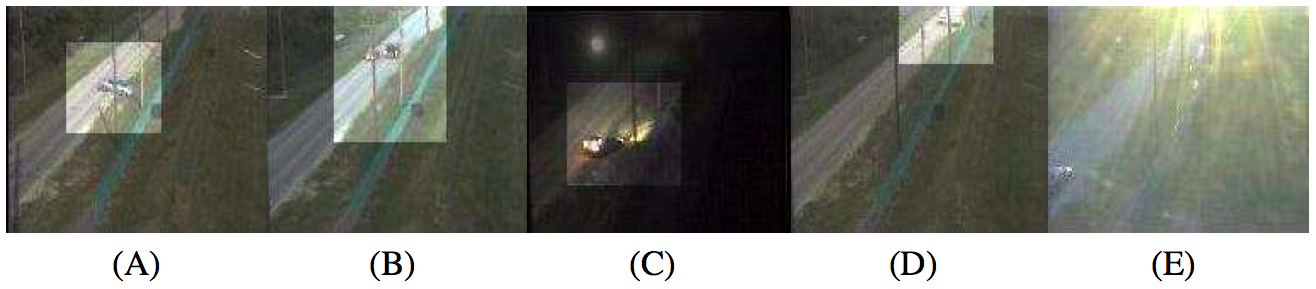
\includegraphics[width=5.5in]{figures/zhong-road-surveillance-video.png} \caption[Zhong
    et al.'s experimental results on road surveillance video.]{\DIFaddFL{Zhong
    et al.'s experimental results on road surveillance video.  Usual
    events consist of cars moving along the road. Correctly detected
    unusual events include: (A) cars pulling off the road, (B) cars
    stopping and backing up, (C) cars making U-turns and people
    walking on the road. Undetected unusual events include: (D) cars
    stopping on the far end, due to coarseness of the spatial
    features. Reprinted from Zhong et al.}\
    \DIFaddFL{(2004).}}  \label{fig:zhong-work}
\end{figure}

\shortciteA{georis04video} \DIFadd{build a real-time bank agency monitoring system. 
The scenarios are modeled 
by domain expert knowledge. End-user feedback is collected to improve the 
scenario models. Figure \ref{fig:georis-work} shows a scenario of a coordinated 
bank attack of multiple robbers.

}

\begin{figure}[t]
    \centering
    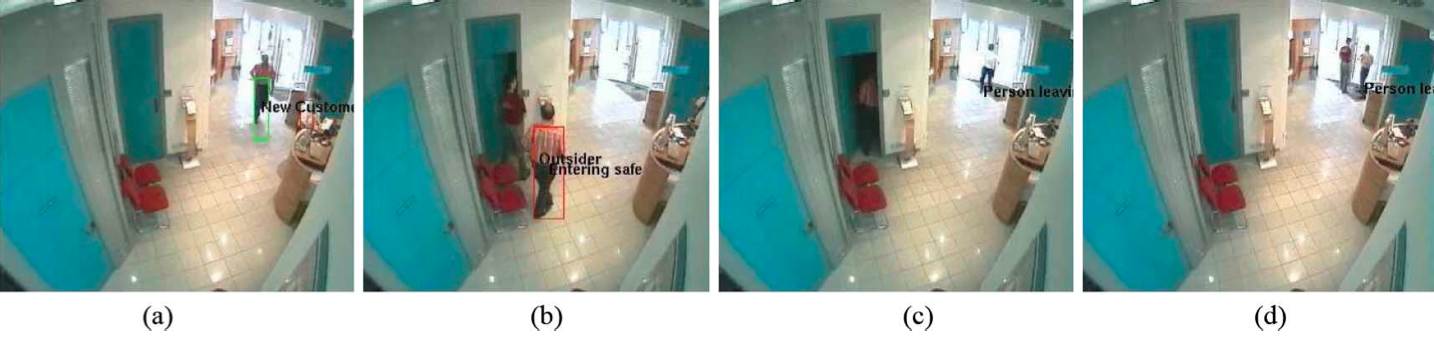
\includegraphics[width=5.5in]{figures/georis-bank-attack.png}
    \caption[Example video of a simulated bank attack.]
        {\DIFaddFL{Example video of a simulated bank attack. (a) Person enters the bank. 
        (b) Robber is identified to be an outsider. Robber is entering the 
        bank safe. (c) A customer leaves the bank. (d) Robber leaves the bank. 
        Reprinted from Turaga et al.}\ \DIFaddFL{(2008).}\mbox{%DIFAUXCMD
\nocite{turaga08survey}
}%DIFAUXCMD
}
    \label{fig:georis-work}
\end{figure}

\shortciteA{vaswani05activity} \DIFadd{use a statistical model such as a 
continuous-state hidden Markov model (HMM) for the configuration of 
a set of landmark shape dynamics in an activity. They identify an 
abnormal activity defined 
as a change in the shape activity model. Their approach is used in 
an airport scenario with people deplaning and moving toward the 
terminal. Figure \ref{fig:vaswani-work} shows an example of people 
deplaning.

}

\begin{figure}[t]
    \centering
    \subfloat[]{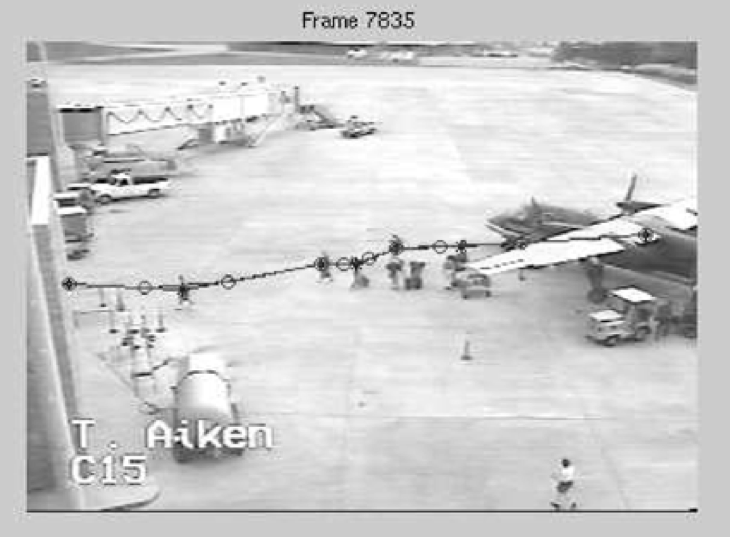
\includegraphics[width=2in]{figures/vaswani-normal-activity.png}}
    \DIFaddFL{\hspace{0.03in}
    }\subfloat[]{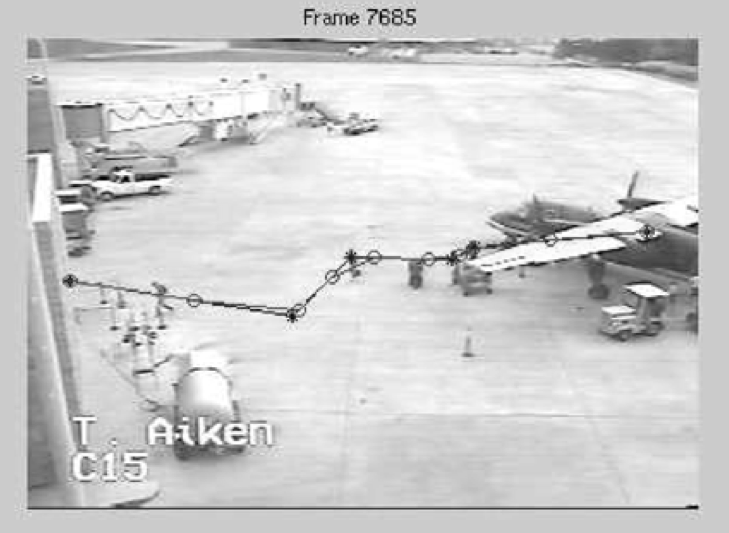
\includegraphics[width=2in]{figures/vaswani-abnormal-activity.png}}
    \caption[Vaswani et al.'s experimental results on an airport scenario.]
        {\small \DIFaddFL{Vaswani et al.'s 
        experimental results on an airport scenario. (a) A ``normal activity'' 
        frame with 4 people. 
        (b) Abnormality introduced by making one person walk-away in an 
        abnormal direction. Reprinted from Vaswani et al.}\ \DIFaddFL{(2005)}}
    \label{fig:vaswani-work}
\end{figure}

\DIFaddend \section{Contributions}

The contributions of this dissertation are as follows.

\begin{enumerate}
  \item We propose an intelligent video surveillance system that is
    practical and fairly close to the ideal surveillance system, which
    should monitor \DIFdelbegin \DIFdel{and automatically raise }\DIFdelend \DIFaddbegin \DIFadd{activity and automatically trigger }\DIFaddend alarms to security
    personnel;

  \item We develop an algorithm for extracting and tracking multiple 
    moving foreground blobs in a scene using an appearance model;

  \item We propose a shadow detection method that uses a simple
    maximum likelihood classification approach based on color
    information;

  \item We propose a new method for clustering human behaviors that 
    is suitable for bootstrapping an anomaly detection module for 
    intelligent video surveillance systems;

  \item We propose and develop a new and effective algorithm for
    semi-supervised learning of common human behaviors and detect 
    anomalies in video sequences;

  \item We introduce a new and more accurate algorithm for
    incrementally profiling human behaviors in video sequences without
    requiring storage of large databases of training data;

  \item We provide the source code and datasets
    online\footnote{See \url{http://www.kanouivirach.com/#downloads}.}
    for researchers interested in evaluating or extending our work.
\end{enumerate}

\subsection{List of Publications}

We provide a list of publications as part of this dissertation. We
also include the list of works currently under review and preparation
for submission.

\subsection*{Published Works}

\begin{itemize}
  \renewcommand\labelitemi{--} 

  \item \DIFaddbegin {\bf{Extracting the Object from the Shadows: Maximum
    Likelihood Object/Shadow Discrimination}}\\ \DIFadd{Kan Ouivirach and
    Matthew N.}\ \DIFadd{Dailey}\\ \textit{\DIFadd{International Conference on
    Electrical Engineering/Electronics Computer Telecommunications and
    Information Technology (ECTI-CON)}}\DIFadd{, pages 1--5, 2013}\\ 
    \DIFadd{Publisher: IEEE Computer Society}\\ \DIFadd{Included in 
    Chapter~\ref{ch:shadow}

}

  \item \DIFaddend \textbf{Clustering Human Behaviors with Dynamic Time Warping
    and Hidden Markov Models for a Video Surveillance
    System}\nocite{kan10clustering}\\ Kan Ouivirach and Matthew N.\
    Dailey\\ \textit{International Conference on Electrical
    Engineering/Electronics Computer Telecommunications and
    Information Technology (ECTI-CON)}, pages 884--888, 2010\\
    Publisher: IEEE Computer Society\\ Included in
    Chapter~\ref{ch:clustering}\\

  \item \textbf{Automatic Suspicious Behavior Detection from a Small
    Bootstrap Set}\nocite{kan12detection}\\ Kan Ouivirach, Shashi
    Gharti, and Matthew N.\ Dailey\\ \textit{International Conference
    on Computer Vision Theory and Applications (VISAPP)}, volume 1,
    pages 655--658, 2012\\ Publisher: Springer-Verlag\\ Included in
    Chapter~\ref{ch:batch}\\

  \item \textbf{Incremental Behavior Modeling and Suspicious Activity
    Detection}\nocite{kan13incremental}\\ Kan Ouivirach, Shashi
    Gharti, and Matthew N.\ Dailey\\ \textit{Pattern Recognition},
    46(3): 671--680, 2013\\ Publisher: Elsevier\\ Included in
    Chapter~\ref{ch:incremental}
  
\DIFdelbegin %DIFDELCMD < 

%DIFDELCMD < \end{itemize}
%DIFDELCMD < 

%DIFDELCMD < %%%
\subsection*{\DIFdel{Manuscripts Currently under Review}}

%DIFAUXCMD
%DIFDELCMD < 

%DIFDELCMD < \begin{itemize}
%DIFDELCMD <   \renewcommand\labelitemi{--}
%DIFDELCMD < 

%DIFDELCMD <   \item {\bf{Extracting the Object from the Shadows: Maximum
%DIFDELCMD <     Likelihood Object/Shadow Discrimination}}\\ %%%
\DIFdel{Kan Ouivirach and
    Matthew N.}%DIFDELCMD < \ %%%
\DIFdel{Dailey}%DIFDELCMD < \\ %%%
\textit{\DIFdel{International Conference on
    Electrical Engineering/Electronics Computer Telecommunications and
    Information Technology (ECTI-CON)}}%DIFAUXCMD
\DIFdel{, 2013}%DIFDELCMD < \\ %%%
\DIFdel{Publisher: IEEE
    Computer Society}%DIFDELCMD < \\ %%%
\DIFdel{Included in Chapter~\ref{ch:shadow}

}\DIFdelend 

\end{itemize}

\subsection*{Manuscripts Currently in Preparation}

\begin{itemize}
  \renewcommand\labelitemi{--}

  \item {\bf{Incorporating Geometric and Shadow Region Shape
    Information for Shadow Detection}}\\ Kan Ouivirach and Matthew N.\
    Dailey\\ To be submitted in \textit{International Conference on
    Computer Vision and Pattern Recognition (CVPR)}, 2013\\ Publisher:
    IEEE Computer Society

\end{itemize}

\section{Organization of Dissertation}

I organize the rest of this dissertation as follows.

In Chapter \ref{ch:blobanalysis}, I describe our blob-based motion
analysis methods including blob extraction and appearance-based blob
tracking.

In Chapter \ref{ch:shadow}, I present a new method for detecting
shadows using a simple maximum likelihood classification method based
on color information.

In Chapter \ref{ch:clustering}, I propose a new method for clustering
behaviors in a scene.

In Chapter \ref{ch:batch}, I present an automatic suspicious behavior
detection method that uses a small bootstrap set.

In Chapter \ref{ch:incremental}, I describe our extension of the
suspicious behavior detection approach for incremental learning in
which security personnel feedback is incorporated.

Finally, in Chapter \ref{ch:conclusion}, I conclude and discuss the
possible further extensions of my dissertation.

\FloatBarrier


% --- Maybe use later ---

%(see Figure \ref{fig:zm-console}) 
%\begin{figure}[t]
%  \begin{center}
%    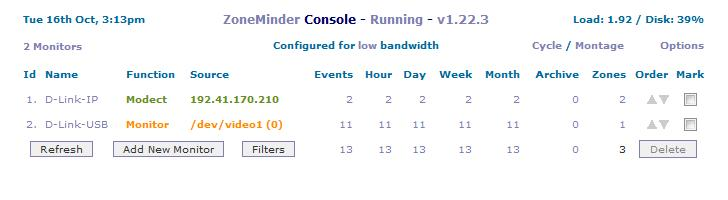
\includegraphics[width=4.5in]{figures/zm-console.jpg}
%    \caption{ZM Console} 
%    \label{fig:zm-console}
%  \end{center}
%\end{figure}

%ZM has three main modules. The first is the ZM Capture (ZMC) module
%whose job is to capture video frames from a video device as quickly as
%possible. The second is the ZM Analysis (ZMA) module, which performs
%video analysis. It finds the captured frames and checks whether the
%detected motion should generate an alarm or not. The last is the ZM
%Frame (ZMF) module. It is an optional module for writing the captured
%frames to file system. This module could potentially reduce the
%workload of ZMA, so ZMA can do more analysis work. If ZMF is not
%enabled, ZMA will write captured frames to file system instead.

%The core of ZM supports capturing and analyzing images. It also
%provides a configurable set of parameters (see
%Figure \ref{fig:zm-option}). ZM allows us to define ``zones'' for each
%camera and vary the sensitivity and functionality (see
%Figure \ref{fig:zm-webcam01-zones}
%and \ref{fig:zm-webcam01-zones-define}). Therefore, we can eliminate
%unnecessary regions and set the different thresholds for each zone. ZM
%also provides a motion detection feature for detecting changes in a
%scene and setting an alarm based on the user-defined threshold.

%\begin{figure}[t]
%  \begin{center}
%    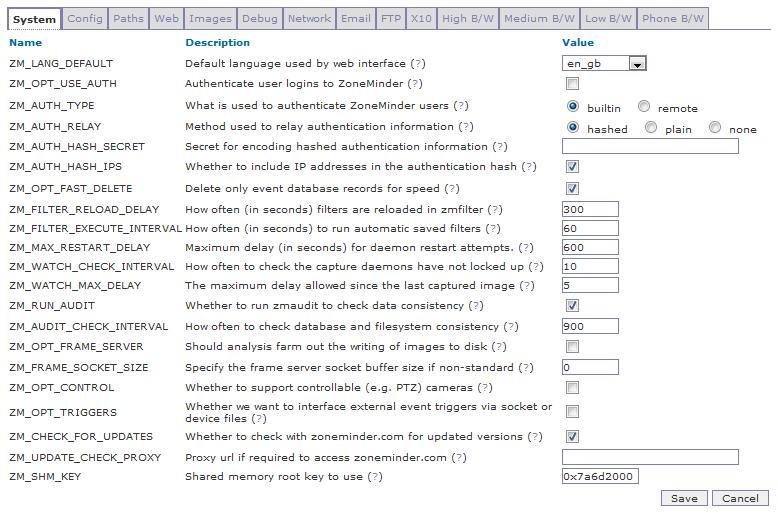
\includegraphics[width=4.5in]{figures/zm-options.jpg}
%    \caption{ZM Options}
%    \label{fig:zm-option}
%  \end{center}
%\end{figure}

%\begin{figure}[t]
%  \begin{center}
%    \subfloat[]{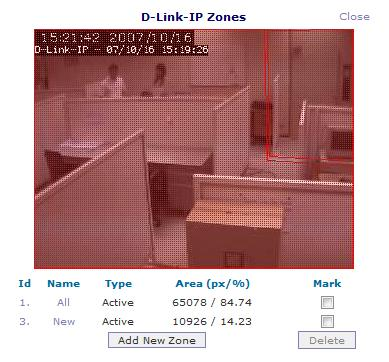
\includegraphics[scale=0.5]{figures/zm-webcam01-zones.jpg}\label{fig:zm-webcam01-zones}}
%    \hspace{0.1in}
%    \subfloat[]{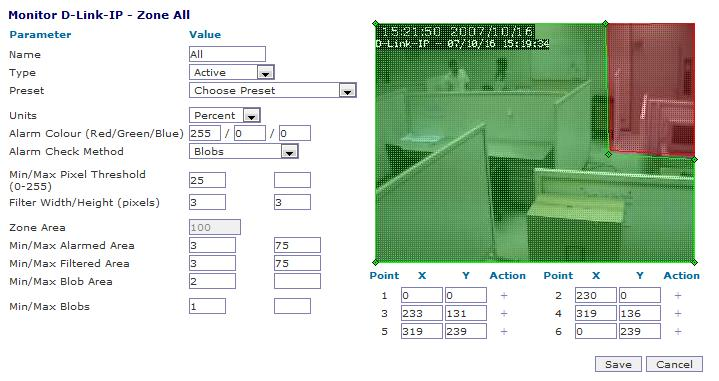
\includegraphics[scale=0.5]{figures/zm-webcam01-zones-define.jpg}\label{fig:zm-webcam01-zones-define}}
%  \end{center}  
%  \caption[Example of zone defined in ZoneMinder]{Example of (a) zone
%  defined and (b) configuring a zone in ZoneMinder.}
%  \label{fig:zm-webcam-zones}
%\end{figure}

%Here I review only the intrusion detection module.  
%The intrusion detection module automatically detects prohibited
%intrusion behaviors while ignoring distractions that cause false
%alarms, like small animals, swaying branches,
%etc. Figure \ref{fig:intrusion-detection} shows a screen shot of the
%result from this module. This module can be used on stationary cameras
%as well as on PTZ cameras. There are two modes which are Regional
%Entrance and Tripwire. The first mode provides a security alarm when
%the system detects a person or vehicle moving within a prohibited
%area. The second mode provides a security alarm when a person or
%vehicle breaks through a demarcation line. User can configure this
%mode to prohibit any crossover or to allow movement in a single
%direction.

%\begin{figure}[t]
%  \begin{center}
%    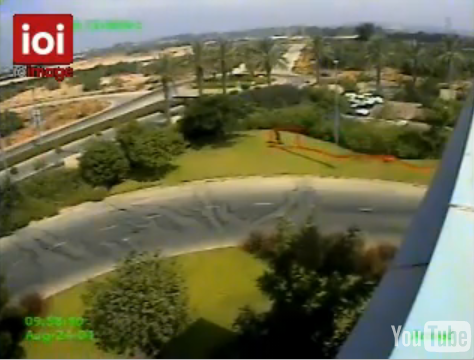
\includegraphics[width=3in]{figures/intrusion-detection.png}
%     \caption[Screen shot of DVTel's intrusion detection
%     module]{Screen shot of DVTel's intrusion detection
%     module. Captured from the video demonstration on DVTel's Web
%     site.}
%    \label{fig:intrusion-detection}
%  \end{center}
%\end{figure}

%For example, it has the knowledge that a head contains two
%eyes and a mouth; so, if either an eye or mouth is detected, it will
%assume that there is a head at that position. Vitamin D Video trained
%a learning network with several hundred videos of humans. Also,
%examples of vehicles and animals not people are trained. As a result,
%Vitamin D Video can tolerate to real world problems.

\setlength{\footskip}{8mm}

\chapter{Blob-Based Motion Analysis}
\label{ch:blobanalysis}

\textit{In this chapter, I review existing blob-based motion analysis
approaches including blob extraction, blob feature extraction, and
blob tracking. I provide details of our methods, and then I discuss
the feasibility of further improvement.}

\section{Introduction}

Motion analysis is the first key step in human behavior understanding,
since the results of later processes such as activity recognition rely
on the analysis.  Motion analysis provides a detailed synopsis of
object movement in the scene, on which foundation we can interpret the
activities in a surveillance video. This could save a tremendous
amount of human effort in monitoring or retrieving videos for review.

This dissertation focuses exclusively on blob-based motion analysis
methods. Our method assumes the camera is fixed relative to the scene
in which objects/people are moving.

\section{Literature Review}

In this section, I provide a review of existing methods for blob-based
motion analysis. The section is divided into three parts. The first
part is blob extraction, the second part is blob feature
extraction, and the last part is blob tracking.

\subsection{Blob Extraction}

Many approaches can be used to extract blobs or objects from a scene,
assuming the camera is fixed. The simplest approach is image
differencing. \shortciteA{yamato92hmm} use this method to extract
blobs representing humans in a scene based on the following
conditions:
\[
  \begin{array}{lc}
    {\rm if} & |{I_a (x,y) - I_b (x,y)}|< T,\;I_e (x,y) = 0 \\ 
    {\rm else} & I_e (x,y) = I_a (x,y).
  \end{array}
\]
$I_e (x,y)$ is the extracted human image, $I_a (x,y)$ is the original
image, $I_b (x,y)$ is a background image without any objects, and $T$
is a predefined threshold. This method can work well under specific
conditions but is not robust to noise, due to the use of a static
background image. In real-world situations, the background scene
changes over time.

\shortciteA{nair02surveillance} improve the image differencing 
technique by updating the background model and threshold over time for
every frame using temporal averaging. They first model the background
by taking the average of five consecutive frames without any object in
the scene. The labeled pixels are considered as foreground if they
satisfy the following condition:
\[
  |{I_n (x,y) - B_n (x,y)}| > T_n (x,y),
\]
where $I_n (x,y)$ is the current frame, $B_n (x,y)$ is the current
background model, and $T_n (x,y)$ is a threshold function. The authors
initialize the threshold value to 50 at all pixel locations. The
background model and threshold function are updated as follows:
\[
  \begin{array}{ll}
    B_{n + 1} (x,y) = \left\{ 
    \begin{array}{l}
      B_n (x,y) \\ 
      \alpha B_n (x,y) + (1 - \alpha )I_n (x,y) 
    \end{array} \right.
    &
    \begin{array}{l}
      {\rm if}\;(x,y)\;{\rm is}\;{\rm foreground}, \hfill  \\
      {\rm otherwise}, \hfill 
    \end{array}
  \end{array}
\]
\[
  \begin{array}{ll}
    T_{n + 1} (x,y) = \left\{
    \begin{array}{l}
      T_n (x,y) \\ 
      \alpha T_n (x,y) + 2(1 - \alpha)| {I_n (x,y) - B_n (x,y)}|
    \end{array} \right.
    &
    \begin{array}{l}
      {\rm if}\;(x,y)\;{\rm is}\;{\rm foreground}, \hfill  \\
      {\rm otherwise}, \hfill 
    \end{array}
  \end{array}
\]
where $\alpha$ is a constant to determine how fast $B_n (x,y)$ and
$T_n (x,y)$ adapt to changes. The update to $T_{n+1}(x, y)$ increases
the threshold when large variations in the background pixel
distribution are observed and decreases when little variation is
observed.

Although the image differencing technique is fast and commonly used in
many surveillance applications such as
ZoneMinder \shortcite{zoneminder}, a single model with a simple
threshold per pixel may not allow adaptation to multi-modal background
distributions.

Many researchers have attempted to improve background modeling to deal
with cluttered dynamic scenes. \shortciteA{wren97pfinder} model people
and the background scene separately using a single Gaussian
distribution per pixel in the YUV color space. Each pixel is
represented by a vector $[x, y, Y, U, V]^T$, where $(x, y)$ is the
pixel location and $(Y, U, V)$ is the color component. They classify
each pixel by calculating a likelihood for each class and selecting
the best one.  Based on the classification result, they update the new
model's parameters for each person and for the background scene
accordingly.  Using this background modeling technique with the proper
initial parameters yields reasonable results for both indoor and
outdoor scenes. Figure \ref{fig:car-sgm-result} shows sample results
for the single Gaussian background modeling method. Although this
technique can deal with noise, it is unsuitable for more cluttered
dynamic background scenes, especially outdoor scenes in which
multi-modal background distributions occur more frequently.

Several additional methods have been proposed to model backgrounds in
recent years. Examples include an eigenvalue decomposition-based
approach\shortcite{oliver00modeling}, a kernel density
estimation-based approach \shortcite{elgammal02background}, and a
median-based approach \shortcite{li06behavior}.

One of the best-known background modeling techniques is that
of \shortciteA{stauffer99background}, who propose a method that models
multi-modal background distributions using a mixture of Gaussian (MoG)
distributions. This technique works well in many cluttered dynamic
scenes. It also outperforms the single Gaussian background modeling
method outdoors, since multi-modal background distributions occur
frequently in outdoor scenes. The authors model the recent history of
each pixel using a mixture of $K$ Gaussian distributions. $K$ is
determined by the available memory and computational power. They
classify pixel values that do not fit one of the background
distributions as foreground until one of the Gaussian distributions
supports those values. Figure \ref{fig:car-mog-result} shows sample
results for the MoG background modeling method.

\begin{figure}[t]
  \centering
  \subfloat[]{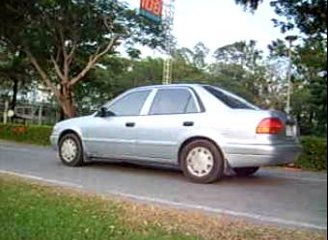
\includegraphics[scale=0.5]{figures/car-original.jpg}
  \label{fig:car-original}}
  \hspace{0.1in}
  \subfloat[]{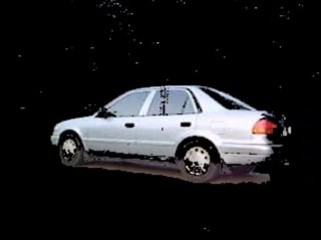
\includegraphics[scale=0.5]{figures/car-sgm-result.jpg}
  \label{fig:car-sgm-result}}
  \hspace{0.1in}
  \subfloat[]{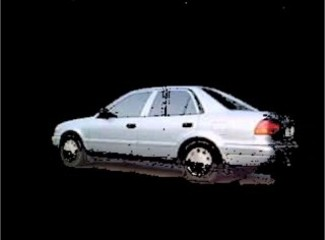
\includegraphics[scale=0.5]{figures/car-mog-result.jpg}
  \label{fig:car-mog-result}}
  \caption[Example results for single and MoG background modeling
    methods.]  {\small Example results for single and MoG background
    modeling methods. (a) Original image. (b) Foreground pixels using
    the single Gaussian background modeling method. (c) Foreground
    pixels using the MoG background modeling method. Reprinted from
    Tuan Anh (2008)\nocite{anh08thesis}.}
  \label{fig:bck-model-results}
\end{figure}

However, the MoG background modeling method faces problem \DIFdelbegin \DIFdel{ห }\DIFdelend dealing
with gradual illumination changes, as seen in
Figure \ref{fig:poppe-mog-result}. \shortciteA{poppe07background}
propose a new version of the MoG background modeling method to solve
this problem. The idea is to store the previous pixel value and
previous matching model number and use them in the matching step. In
the matching step, each pixel is checked against the $K$ Gaussian
distributions. For the model that matches the pixel in the previous
frame, if the difference between the current pixel value and previous
pixel value is smaller than a threshold, an intermediate match is
defined; otherwise, the normal matching step is followed. If the
matched model represents the background, the model number and the
current pixel value are stored; otherwise, they retain their
values. By doing this, foreground objects will not affect the recent
history. Figure \ref{fig:poppe-bck-model-results} shows example
results of using the MoG background modeling method and Poppe et al.'s
improved MoG background modeling method.

\begin{figure}[t]
  \centering
  \subfloat[]{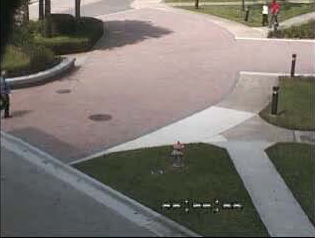
\includegraphics[scale=0.5]{figures/poppe-original.png}
  \label{fig:poppe-original}}
  \hspace{0.1in}
  \subfloat[]{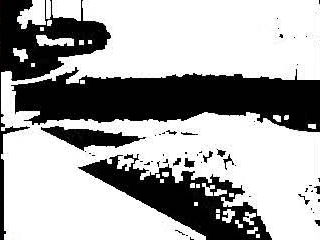
\includegraphics[scale=0.5]{figures/poppe-mog-result.png}
  \label{fig:poppe-mog-result}}
  \hspace{0.1in}
  \subfloat[]{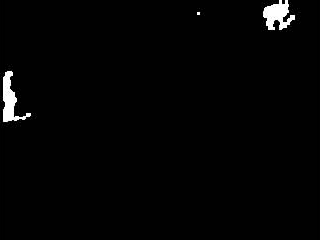
\includegraphics[scale=0.5]{figures/poppe-improved-mog-result.png}
  \label{fig:poppe-improved-mog-result}}
  \caption[Example MoG and improved MoG background modeling
    results.]{\small Example MoG and improved MoG background modeling
    results. (a) Original image. (b) Foreground pixels using MoG
    background modeling. (c) Foreground pixels using improved MoG
    background modeling. Reprinted from Poppe et al.\ (2007).}
  \label{fig:poppe-bck-model-results}
\end{figure}

Once the foreground is segmented from the background, moving blobs can
be extracted as connected components in the foreground mask.

\subsection{Blob Feature Extraction}

After segmenting blobs, we need to extract features to describe the
shape and dynamics of each blob. Extracted features are commonly used
in the blob tracking and behavior understanding processes.  In this
section, I review blob feature extraction methods used in existing
systems.

\shortciteA{yamato92hmm} extract mesh features from foreground
blobs. Mesh features are low-level image features that have also been
successfully applied to complex 2D patterns such as multi-font
characters \shortcite{umeda82font}. Each binarized image ($M \times N$
pixels) is divided into a mesh with $M_M \times N_M$ cells. They
represent each binarized image by a feature vector in which each
element is the proportion of black pixels in each
cell. Figure \ref{fig:mesh-feature} shows how mesh features are
calculated.

\begin{figure}[t]
  \centering
  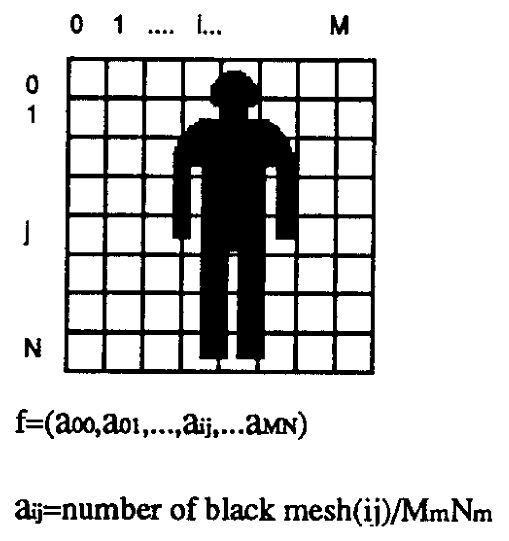
\includegraphics[width=2in]{figures/mesh-feature.jpg}  
  \caption[Mesh feature calculation.]{\small Mesh feature
    calculation. Reprinted from Yamato et al.\ (1992).}
  \label{fig:mesh-feature}
\end{figure}

\shortciteA{nair02surveillance} represent an extracted blob by a
feature vector that contains the coordinates of the blob's center of
mass, average color, and height. They use a $k$-means algorithm to
compute a set of codebook vectors from a set of feature vectors in the
training data. Once the $k$-means model is trained, they map a feature
vector to the index of the nearest codebook vector using Euclidean
distance. They then generate and output a sequence of codebook
vectors, which are then input to behavior modeling.

Star skeletonization is a technique that represents the gross
extremity structure of a blob. For humans, the gross extremities would
normally be the head, arms, and legs. \shortciteA{fujiyoshi98motion}
use this technique for analyzing human
motion. Figure \ref{fig:star-skeleton-example} shows an example of two
different star skeletons extracted from two human motions.

\begin{figure}[t]
  \centering
  \begin{tabular}{c}
    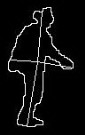
\includegraphics{figures/star-walking-01.jpg} 
    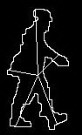
\includegraphics{figures/star-walking-02.jpg} 
    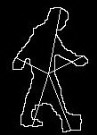
\includegraphics{figures/star-walking-03.jpg} 
    
\includegraphics{figures/star-walking-04.jpg} \\
    (a) \\
    
\includegraphics{figures/star-sit-01.jpg} 
    
\includegraphics{figures/star-sit-02.jpg} 
    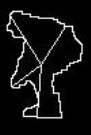
\includegraphics{figures/star-sit-03.jpg} 
    
\includegraphics{figures/star-sit-04.jpg} \\
    (b)
  \end{tabular}
  \caption[Example star skeletons.]{\small Example star skeletons
    extracted from two human motions. (a) Walking. (b) Leaning forward
    and sitting down. Reprinted from Tuan Anh
    (2008)\nocite{anh08thesis}.}
  \label{fig:star-skeleton-example} 
\end{figure}

Some feature extraction methods have the ability to capture motion
history rather than only capturing current static features.  One such
method is space-time image features. \shortciteA{li06behavior} propose
a method based on space-time image features for automatic behavior
modeling and recognition. Their method is simple and insensitive to
noise, and it does not need to track parts of the human body. They
represent object shape using space-time images. After the foreground
is extracted, they equidistantly divide the bounded rectangle of the
foreground into $10\times7$ sub-blocks then normalize the value of
each sub-block as follows:
\[
  d_i = \left\lfloor {\frac{{s_i}}{{M}}\times255} \right\rfloor, i =
    1,2, \ldots,k,
\]
where $k=10\times7$ is the number of sub-blocks; $s_i$ is the number
of foreground pixels in the $i^{th}$ sub-block, and $M$ is the maximum
value of $s_i$, where $i=1,2,...,k$. The resulting shape descriptor
$D_t$ at image frame $t$ is defined as $D_t =
[d_1,d_2,d_3,...,d_k]$. To represent the motion of a sequence with $t$
frames, they construct the space-time image representation (see
Figure \ref{fig:space-time-feature}) as a matrix $I$ of size $t\times
k$:
\[
  I = [D_1,D_2,D_3, \ldots ,D_t]^{T}_{t\times k}
\]
They then extract the features from this representation by Gabor
filtering as follows:
\[
  F_n (x,y) = \iint {I_n (x_1 ,y_1 )G(x - x_1 ,y - y_1 ,f)dx_1dy_1},
\]
\[
  G(x,y,f) = \frac{1}{{2\pi \sigma _x \sigma _y }}\exp \left[ {
  - \frac{1}{2}\left( {\frac{{x^2 }}{{\sigma _x^2 }} + \frac{{y^2
  }}{{\sigma _y^2 }}} \right)} \right]M(x,y,f),
\]
\[
  M(x,y,f) = \cos \left[ {2\pi f(x\cos \theta +
  y\sin \theta)} \right],
\]
where $I_n(x,y)$ is the $n^{th}$ space-time image; $F_n(x,y)$ is the
filtered space-time image; the space constants of the Gaussian
envelope along the $x$ and $y$ axis are represented by $\delta _x$ and
$\delta _y$, respectively, and $f$ is the frequency of the sinusoid
and $\theta$ is the orientation of the Gabor filter.

\begin{figure}[t]
  \centering
  \begin{tabular}{cc}
    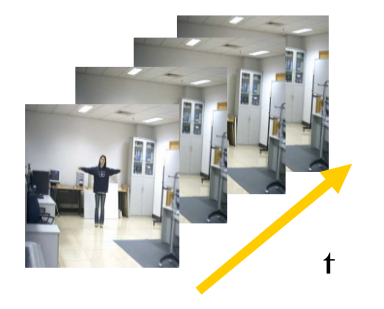
\includegraphics[width=2in]{figures/space-time-original.png} &
    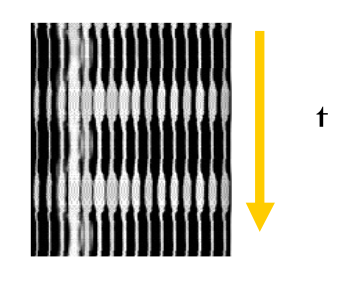
\includegraphics[width=2in]{figures/space-time-image.png} \\
    (a) & (b)
  \end{tabular}
  \caption[Space-time image representation.]{\small Space-time image
    representation. (a) Original video sequence. (b) Space-time image
    for the ``hand clapping'' behavior. Reprinted from H.\ Li et al.\
    (2006).}
  \label{fig:space-time-feature}
\end{figure}

Finally, H.\ Li et al.\ extract statistical features in each
$4 \times 5$ block of each short space-time image. The feature value
is the mean:
\[
  m = \frac{\displaystyle\sum_B | F_n(x, y)|}{K},
\]
where $B$ is a $4 \times 5$ block in the short space-time images, and
$K$ is the number of pixels in blob $B$. Each short space-time image
$V_i$, where $1 \le i \le N$, is represented as a $16 \times 14$
feature vector:
\[
  V_i = [M_1, M_2, \ldots, M_n, \ldots, M_{16}]^T,
\]
where $M_n = (m_{n1}, m_{n2}, \ldots, m_{ni}, \ldots, m_{n14})$.

\shortciteA{davis97mhi} propose a feature extraction method using
motion history image (MHI). MHI is a static image template where pixel
intensity is a function of the recency of motion in the video
sequence. The idea is to represent how the object is moving. The MHI
is defined as:
\[
  \begin{array}{ll}
    H_\tau (x,y,t) = \left\{ 
    \begin{array}{l}
      \tau \\ 
      \max (0, H_\tau (x, y, t - 1) - 1)
    \end{array} \right.
    &
    \begin{array}{l}
      {\rm if}\;D(x, y, t) = 1, \hfill  \\
      {\rm otherwise}, \hfill 
    \end{array}
  \end{array}
\]
where $H_\tau (x,y,t)$ represents the MHI for a pixel $(x,y)$ at time
$t$. The more recently moving pixels will be
brighter. Figure \ref{fig:mhi} presents example MHIs. The more
recently moving pixels are brighter.

\begin{figure}[t]
  \centering
  \begin{tabular}{ccc}
    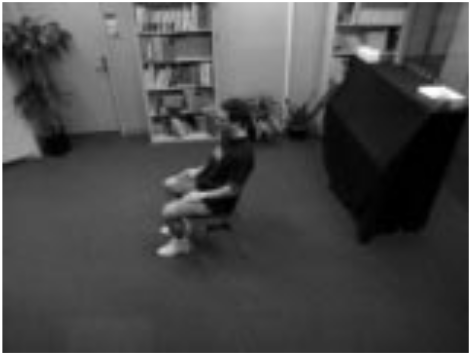
\includegraphics[width=1.5in]{figures/mhi-sit-original.png} &
    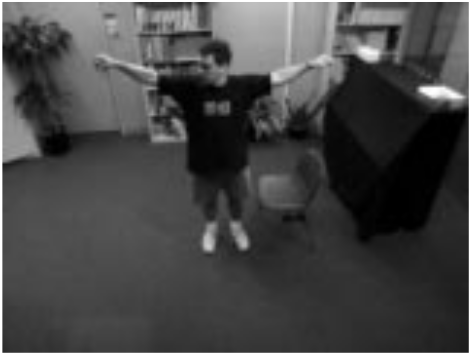
\includegraphics[width=1.5in]{figures/mhi-wave-original.png} &
    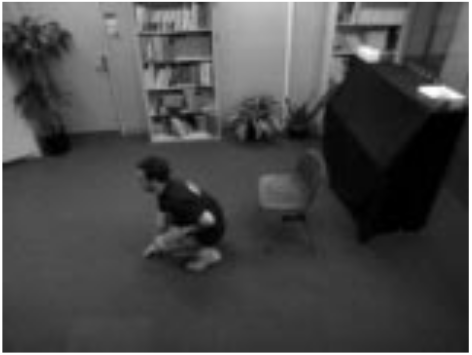
\includegraphics[width=1.5in]{figures/mhi-crouch-original.png} \\
    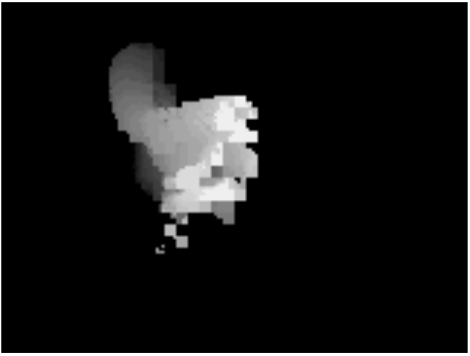
\includegraphics[width=1.5in]{figures/mhi-sit-results.png} &
    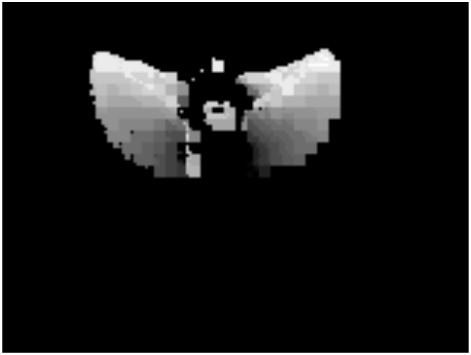
\includegraphics[width=1.5in]{figures/mhi-wave-results.png} &
    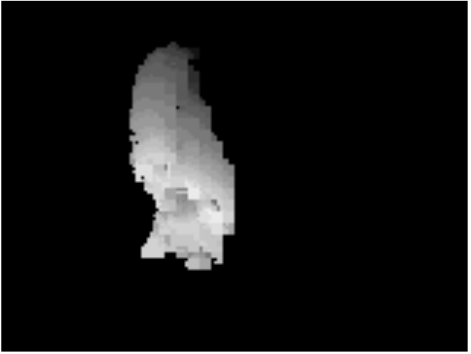
\includegraphics[width=1.5in]{figures/mhi-crouch-results.png} \\
    sit-down & arms-wave & crouch-down 
  \end{tabular}
  \caption[Example motions along with their motion history images
    (MHIs).]{\small Example motions along with their motion history
    images (MHIs). Reprinted from J.\ W.\ Davis and Bobick (1997).}
  \label{fig:mhi}
\end{figure}

Based on the local intensity history of
pixels, \shortciteA{xiang02event} propose a new low-level primitive
applicable to human representation that can describe human actions
efficiently, namely, the pixel change history (PCH).  The PCH is
capable of characterizing pixel-wise temporal visual information in
order to detect pixel-level events. It is a representation of
pixel-wise changes based on a combination of the pixel signal energy
(PSE) proposed by \shortciteA{ng03pixel} and the MHI. The PCH is
computed as follows:
\[
  P_{\varsigma ,\tau } (x,y,t) = \left\{ \begin{array}{l}
  \min (P_{\varsigma ,\tau } (x,y,t - 1) + \frac{{255}}{\varsigma },255)\quad 
  \; {\rm if}\;D(x,y,t) = 1 \\ 
  \max (P_{\varsigma ,\tau } (x,y,t - 1) + \frac{{255}}{\tau },0)\quad \quad 
  {\rm otherwise}, \\ 
  \end{array} \right.
\]
where $P_{\varsigma ,\tau } (x,y,t)$ represents the PCH for a pixel
$(x,y)$ at time $t$, $D(x,y,t)$ indicates foreground regions at time
$t$, $\varsigma$ is an accumulation factor, and $\tau$ is a decay
factor. When the accumulation factor is set to 1, the PCH over the
entire image is equivalent to the MHI. 

\shortciteA{xiang08incremental} use a discrete scene-wide event-based
approach for behavior pattern representation. This approach is
effective for cluttered scenes compared to the trajectory-based
representations used in most existing approaches. Xiang and Gong model
the foreground pixels using PCH \shortcite{xiang02event}, group them
into blobs, and define a scene event if the average PCH value of a blob is
larger than a defined threshold. They then represent a scene event as
a 7-dimensional feature vector
\[
  \vec{f} = [ \bar{x}, \bar{y} , w, h, R_f , M_px, M_py],
\]
where $(\bar{x}, \bar{y})$ is the centroid of the blob, $w$ and $h$
are the width and height of the bounding box associated with the blob,
respectively, $R_f$ is the filling ratio of foreground pixels within
the bounding box, and $(M_px, M_py)$ are a pair of first order moments
of the PCH image within the bounding box. 

Recursive filtering \shortcite{masoud03recognition} is a technique
that encodes motion information such as the speed of the motion within
a short period of time. The idea is to represent the ``recency'' of
the motion. This technique is conceptually similar to the MHI. Let
$I_t$ be the frame at time $t$. The filtered image $F_t$ at time $t$
is defined as follows:
\[
  F_t = \left| {I_t  - M_t } \right|
\]
\[
  M_t = (1 - \beta)M_{t - 1}  + \beta M_t 
\]
\[
  M_0 = I_0 = {\rm Background},
\]
where $t = 1, 2, \cdots, n_i$. If $\beta = 0$, the filtered image
$F_t$ will be the foreground and if $\beta = 1$, $F_t$ will be
equivalent to image differencing. Examples of filtered images are
presented in Figure \ref{fig:f-img}.

\begin{figure}[t]
  \centering
  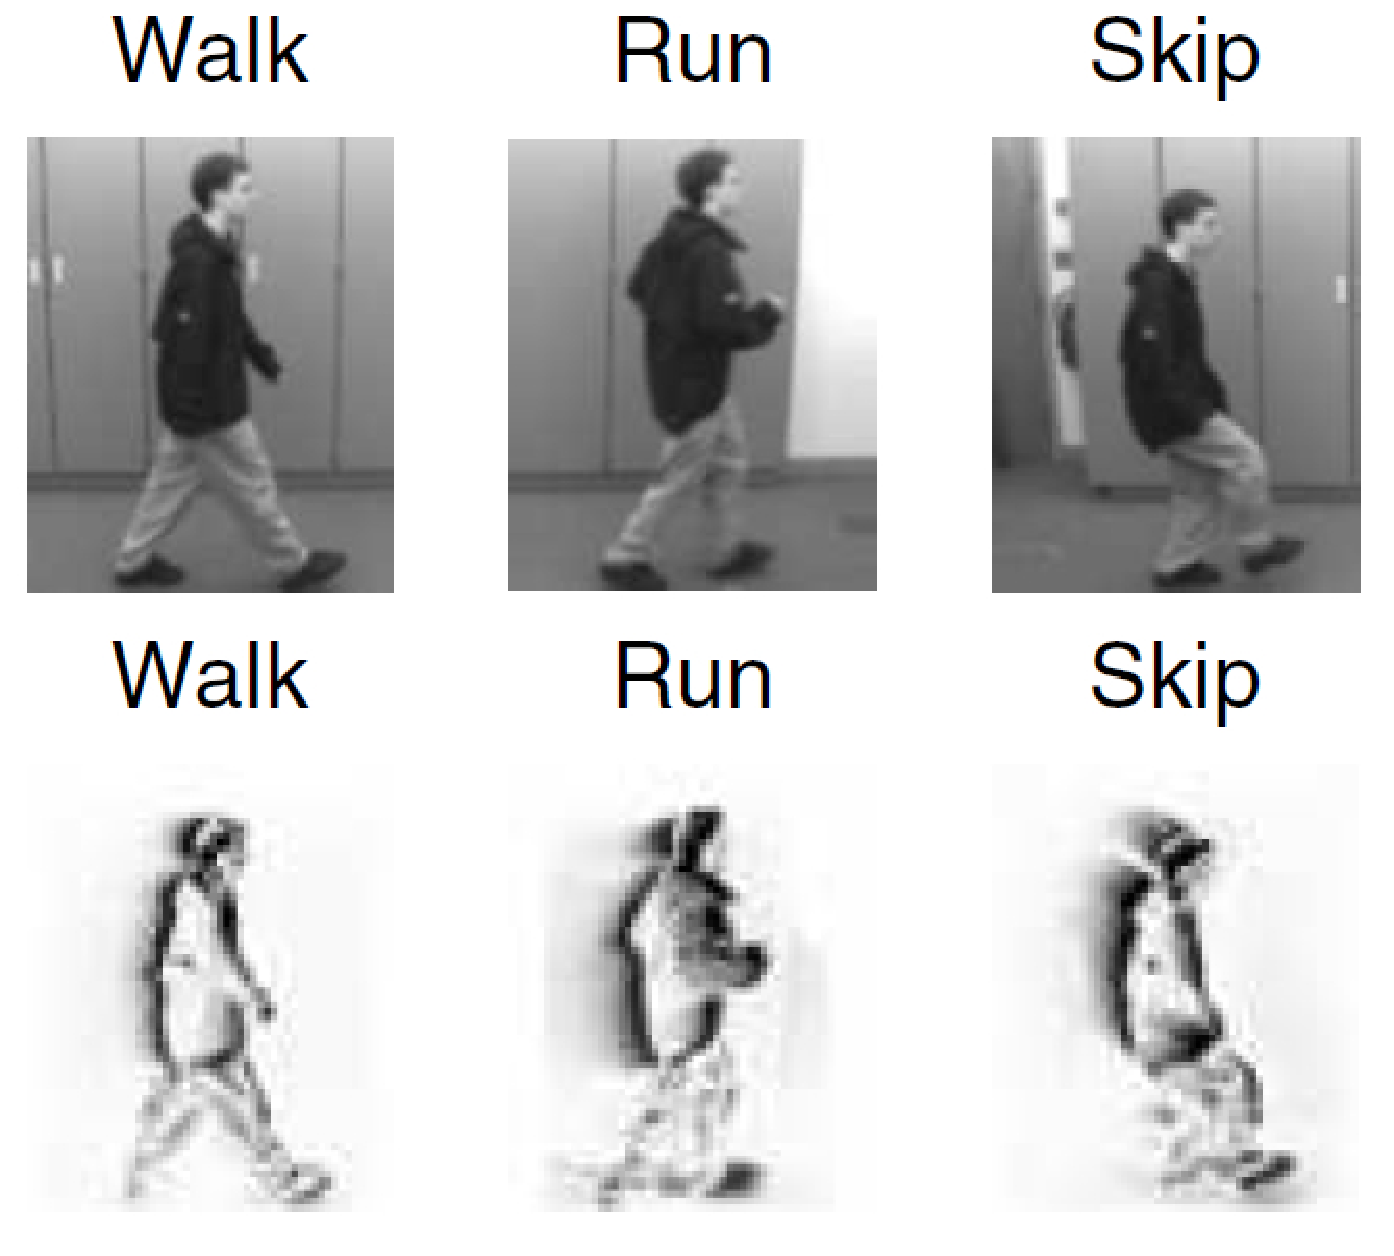
\includegraphics[width=2.5in]{figures/f-img}
  \caption[Example filtered images.]{\small Example filtered
    images. The coefficient $\beta$ is set to 0.5. Reprinted from
    Masoud and Papanikolopoulos (2003).}
  \label{fig:f-img}
\end{figure}

I describe the blob feature representation used in this dissertation
in Section \ref{sec:blob-appearance-based-blob-tracking}.

\subsection{Blob Tracking}

Tracking is one of the most active research areas in computer
vision. It can be used in a variety of applications, e.g.\ video
indexing, sports video enhancement, and visual surveillance.  In the
area of tracking, occlusion ambiguity is the most fundamental
difficulty.  It makes associating blobs with individuals or moving
objects that are partially or fully occluded in different frames
highly challenging, especially in complex scenes.

In video surveillance applications, person/object tracking is a
critical step prior to behavior modeling. Extracted information such
as the motion trajectory can be used to better understand activities
occurring in a scene.

The Kalman filter \shortcite{kalman60filtering} is a well-known
algorithm that has been extensively applied to tracking in many
domains.  In visual surveillance, \shortciteA{rosales99tracking}
propose a method for tracking multiple people in a 3D space. They
assume that the system uses a single uncalibrated video camera to
observe multiple moving people. They use an extended Kalman filter
(EKF) to estimate relative 3D motion trajectories up to a scale
factor.  They select only two feature points, the two opposite corners
of the person's bounding box, to reduce the complexity of the tracking
problem. The 3D size of the person's bounding box is assumed to remain
approximately the same or at least vary smoothly. People are
considered as plane objects, so the depth at both feature points
should be the same. The state vector then becomes:
\[
  \vec{x} = (x_0 ,y_0 ,x_1 ,y_1 ,z\beta ,\dot x_0 ,\dot y_0
  ,\dot x_1 ,\dot y_1 ,\dot z\beta )^T,
\]
where $(x_0, y_0, z\beta)^T$ and $(x_1, y_1, z\beta)^T$ are the
corners of the 3D planar bounding box, and $(\dot x, \dot y, \dot
z\beta)^T$ represents a corner's 3D velocity relative to the
camera. The experimental results demonstrate that Rosales and
Sclaroff's 3D trajectory-based estimation method significantly
improves the robustness over 2D trajectory-based estimation methods.
Figure \ref{fig:rosales-tracking-result} shows an example of 3D
tracking results for this method.

\begin{figure}[t]
  \centering
  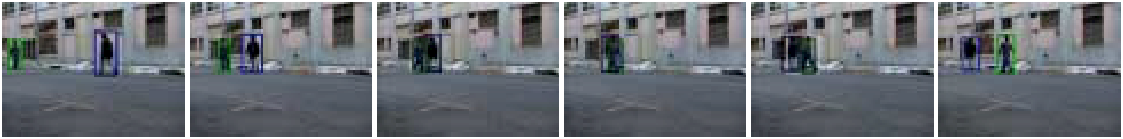
\includegraphics[width=6in]{figures/rosales-tracking-result.png}
  \caption[Sample 3D tracking results from Rosales and Sclaroff's
    method.]{\small Sample 3D tracking results from Rosales and
    Sclaroff's method. Two people walking along different trajectories
    then occluding each other. Reprinted from Rosales and Sclaroff
    (1999).}
  \label{fig:rosales-tracking-result}
\end{figure}

\shortciteA{bodor03recognition} develop an automated system to track
the positions of individual pedestrians using a Kalman filter and
alert security personnel when a pedestrian enters a secure area.

\shortciteA{niu03tracking} propose a method using a second-order
Kalman filter to track each person individually and handle occlusion
problems. They define a state that includes position, velocity, and
acceleration. When a new person is detected, they store a unique label
for that person having the information: height, centroid, and the
average intensity value of the region of the person. They then use
this information to continue keeping track of the person in each
frame.

\shortciteA{girondel04tracking} propose a multiple human tracking
method using the Kalman filter. They define a Kalman filter for each
person then predict the person's bounding box, the person's face's
bounding box, and the speed. They use a state vector of ten components
for each Kalman filter: the corners of the bounding boxes of the
person and face plus two components for face speed. They use skin
detection to detect face and hands and assume that face is a bigger
blob that moves more steadily. In this paper, they use the combination
of a forward tracking phase and a backward tracking phase to track
between detected objects on two consecutive frames. This technique is
also called ``forward and backward overlapping.'' I hereinafter
describe this technique in more details in
Section \ref{sec:blob-appearance-based-blob-tracking}.
Figure \ref{fig:girondel-tracking-result} shows an example of the
tracking results from Girondel et al.'s method.

\begin{figure}[t]
  \centering
  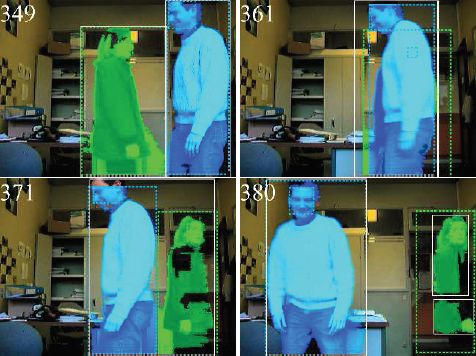
\includegraphics[width=2in]{figures/girondel-tracking-result.png}
  \caption[Sample tracking results from Girondel et al.'s
    method.]{\small Sample tracking results from Girondel et al.'s
    method. Reprinted from Girondel et al.\ (2004).}
  \label{fig:girondel-tracking-result}
\end{figure}

\shortciteA{lv06leftluggage} use a Kalman filter to track moving
blobs. The authors use a color histogram as an appearance model to
resolve the identity problem of blob merging. If the blob in the
current frame matches with multiple existing tracks, they use the
color histogram of each matched track to find the best-corresponding
blob. Figure \ref{fig:lv-blob-tracking-results} shows an example of
blob tracking results from Lv et al.'s method.  Color histograms are a
simple and efficient method that can be used to compare the similarity
of images. However, they lack spatial information. For instance, the
color histogram of an image with single large block of red pixels will
be similar to that of the image with same number of scattered red
pixels.

\begin{figure}[t]
  \centering
  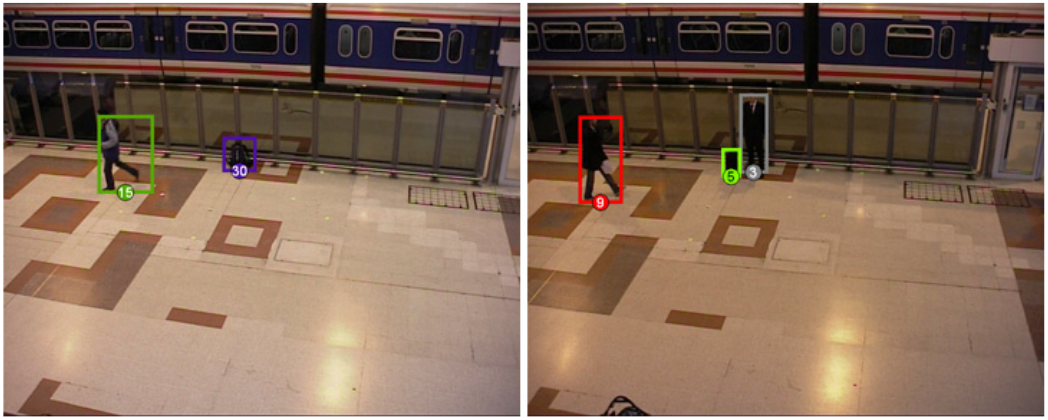
\includegraphics[width=4in]{figures/lv-blob-tracking-results.png}
  \caption[Sample tracking results from Lv et al.'s method.]{\small
    Sample tracking results from Lv et al.'s method. Reprinted from Lv
    et al.\ (2006).}
  \label{fig:lv-blob-tracking-results}
\end{figure}

\shortciteA{senior06tracking} solve occlusion problems by
modeling moving objects using an appearance model. They use an
appearance model to localize objects during partial occlusion, detect
complete occlusions and resolve depth ordering of objects during
occlusions. In this paper, they use a RGB color model as an appearance
model with an associated probability mask for each foreground
blob. The probability mask records the likelihood of the object being
observed at that pixel.  The appearance model of each blob is then
updated on subsequent frames. They also construct a distance matrix by
a bounding box distance measure. Then they use it to determine the
association between tracks and foreground blobs. This technique is
similar to the forward and backward overlap method. In this paper,
they evaluated the proposed method on the PETS 2001 data set, and the
results show that their algorithm successfully deals with complex
real-world interactions. Figure \ref{fig:senior-tracking-results}
shows an example of the tracking results from Senior et al.'s method.

\begin{figure}[t]
  \centering
  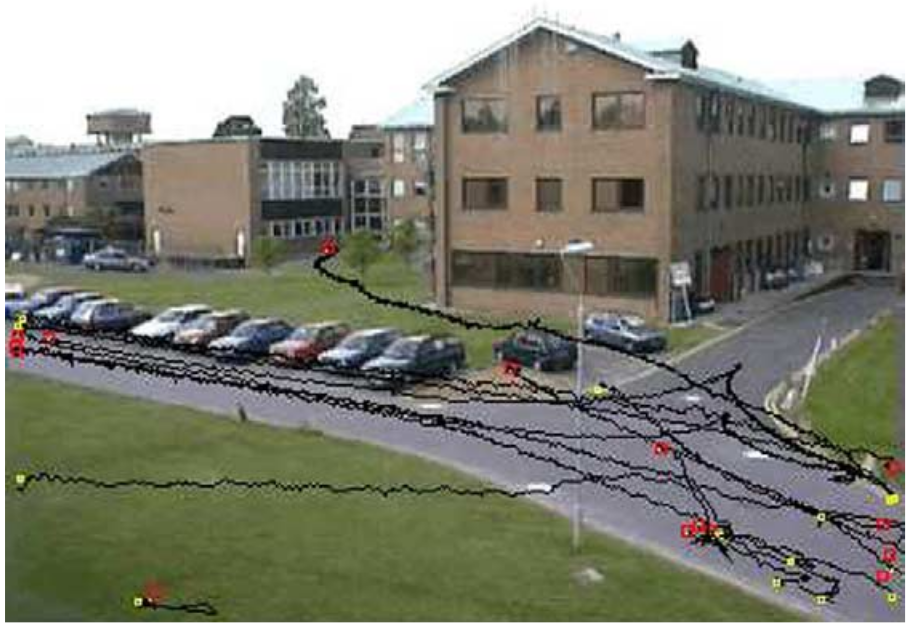
\includegraphics[width=3in]{figures/senior-tracking-results-for-dataset-1.png}
  \caption[Sample tracking results from Senior et al.'s
    method.]{\small Sample tracking results from Senior et al.'s
    method. Reprinted from Senior et al.\ (2006).}
  \label{fig:senior-tracking-results}
\end{figure}

In the following sections, I provide details of our blob-based motion
analysis including global motion detection in
Section \ref{sec:blob-motion-detection}, blob extraction in
Section \ref{sec:blob-blob-extraction}, appearance-based blob tracking
in Section \ref{sec:blob-appearance-based-blob-tracking}, and blob
feature vector discretization in
Section \ref{sec:blob-discretization}. I then finally discuss the
limitations and possible feasibilities for improving our method.

\section{Global Motion Detection}
\label{sec:blob-motion-detection}

Any video frames in which no motion occurs are removed to decrease
processing and storage time. We use simple frame-by-frame
subtraction. When the difference image has a number of pixels whose
intensity differences are above a threshold, we start a new video
segment. We use a threshold large enough not to trigger event
processing in a static scene, e.g.\ when a breeze makes leaves of a
tree move. We also buffer the no-motion frames for a period of time
and include some number of frames before and after the motion in the
event. This method avoids oversegmentation of events when moving
objects stop moving briefly.  In all of the experiments reported in
this dissertation, we start a new video segment when the number of
changed pixels in the 320$\times$240 input exceeds 300.

\DIFaddbegin \DIFadd{Through some preliminary empirical experimentation I found that 300 was a good 
threshold. While this simple approach worked well in our experimental setup, 
it would not work as well in a situation where the camera is subject to 
vibration, causing a large number of pixels to change values significantly.
}

\DIFaddend \section{Blob Extraction}
\label{sec:blob-blob-extraction}

After discarding the no-motion video segments, we use Poppe et al.'s
(2007) background modeling technique\nocite{poppe07background} to
segment foreground pixels from the background. As previously
mentioned, Poppe et al.\ extend the standard mixture of Gaussians
background model
\shortcite{stauffer99background} to handle gradual illumination changes.

\section{Appearance-Based Blob Tracking}
\label{sec:blob-appearance-based-blob-tracking}

\renewcommand{\algorithmicrequire}{\textbf{Input:}}
\renewcommand{\algorithmicensure}{\textbf{Output:}}
\renewcommand{\algorithmicforall}{\textbf{for each}}
\begin{algorithm}
\caption{Appearance-Based Blob Tracking}
\label{blob-tracking-algorithm}
\begin{algorithmic}
  \REQUIRE $B$: set of all current blobs
  \REQUIRE $T$: set of all current tracks
  \REQUIRE $M$: merged track association matrix
  \ENSURE $\widetilde{T}$: set of all revised tracks
  \ENSURE $\widetilde{M}$: revised merged track association matrix
  \STATE $\widetilde{T} \gets \emptyset$; $\widetilde{M} \gets \emptyset$; $L \gets \emptyset$
%  \STATE \COMMENT{Construct an overlap area matrix between the bounding box of blobs and tracks.}
  \STATE $A \gets \textsc{Get-Overlap-Area-Matrix}(B, T)$
  \FORALL{$t \in T$}
    \STATE \textbf{if} $t$ is marked as processed \textbf{then} continue
    \STATE $B' \gets \{ b' \mid A(b', t) > 0 \}$ \COMMENT{$B'$ contains candidate blobs for track $t$.}
    \STATE $T' \gets \{ t \} \cup \{ t' \mid M(t, t') = 1 \}$ \COMMENT{$T'$ contains all tracks currently merged with $t$.}
    \IF{$|B'| \geq 1$}
      \FORALL{$t' \in T'$}
        \STATE Let $b = \displaystyle\argmax_{b' \in B'} S(b', t')$
	\STATE $L \gets L \cup \{ (t', b) \}$
        %\STATE $\widetilde{t} \gets \textsc{Update-Track-Information}(t')$
        %\STATE $\widetilde{T} \gets \widetilde{T} \cup \{ \widetilde{t} \}$
	\STATE $\textsc{Mark-Track-As-Processed}(t')$
      \ENDFOR
%      \STATE Not needed ----- We may need it in case a blob reappears..
%    \ELSE
%      \FORALL{$t' \in T'$}
%         \STATE $s \gets \textsc{Get-Stale-Count}(t')$
%         \IF{$s > \theta_s$}
%           \STATE $\textsc{Mark-Track-For-Deletion}(t')$
%         \ENDIF
%      \ENDFOR
%      \STATE Not needed -----
    \ENDIF
  \ENDFOR
  \FORALL{$(t_i, t_j) \in T \times T$}
    %\STATE \COMMENT{If track $t_i$ links to the same blob $b$ as track $t_j$}
    \STATE If $\exists b$ s.t.\ $(t_i, b) \in L \wedge (t_j, b) \in L, \widetilde{M}_{ij} \gets 1$, otherwise $\widetilde{M}_{ij} \gets 0$
  \ENDFOR
  \STATE $T^* \gets \{ t^* \mid \neg\exists b \in B \;\text{s.t.}\; (t^*,b) \in L \}$ \COMMENT{$T^*$ contains tracks for which ``stale count'' will be increased.}
  \STATE $\widetilde{T} \gets \textsc{Update-Or-Delete-Stale-Tracks}(T,T^*)$
  \STATE $B^* \gets \{ b^* \mid \neg \exists t \in T \;\text{s.t.}\; (t, b^*) \in L \}$ \COMMENT{$B^*$ contains blobs with no tracks assigned.}
  \STATE $\widetilde{T} \gets\textsc{Add-New-Tracks-For-Not-Linked-Blobs}(\widetilde{T},B^*)$
\end{algorithmic}
\end{algorithm}

In this step, we take at time $t$ a list of blobs detected by the
previous step, a set of tracks updated at time $t-1$, and a merged
track association matrix.  We output an updated track list and merged
track association matrix.  Algorithm \ref{blob-tracking-algorithm} is
a pseudocode summary of our approach.  We first construct a matrix in
which each element indicates the overlap area of the bounding box of a
current blob with an existing track.  When a blob is found to
correspond to a single unique track, the track update is simple; we
just associate the blob with the track.  If a track is no longer
visible for some period of time, it will be considered \textit{stale}
and deleted. Special handling is required for cases in which a new
blob overlaps multiple old tracks (\textit{merges}) or multiple new
blobs overlap the same old track (\textit{splits}). To handle these
cases, our method evaluates a similarity function $S(b, t)$ for each
candidate blob-track pair $(b,t)$. $S(b,t)$ is based on the color
coherence vector (CCV; Pass et al., 1996)\nocite{pass96ccv}; when
tracks merge, we group them, but keep their identities separate, and
when tracks split, we associate the new blobs with the correct tracks
or groups of tracks by comparing their CCVs, on the assumption that
when an object eventually separates from the group, its appearance
will be similar to its appearance before the merge.  Our tracking
method performs very well on typical simple cases such as those shown
in Figure \ref{fig:normal-tracking-results} involving clear
trajectories of each moving person or object. However, it still has
some problems with more complex cases such as those shown in
Figure \ref{fig:complex-tracking-results} involving large groups of
people or objects moving together and interacting for some period of
time.

\begin{figure}[t]
  \begin{center}
    \begin{tabular}{ccccc}
      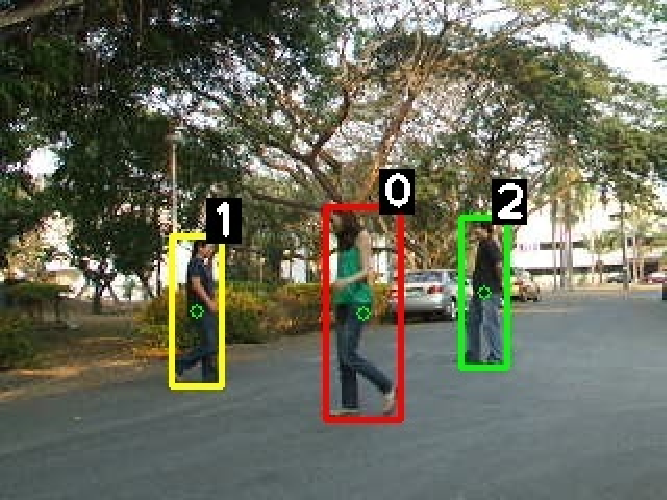
\includegraphics[scale=0.21]{figures/normal-tracking-result-0090.pdf} &
      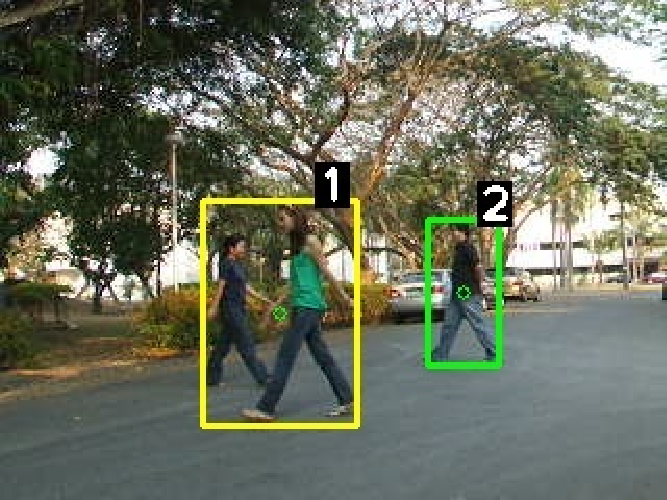
\includegraphics[scale=0.21]{figures/normal-tracking-result-0094.pdf} &
      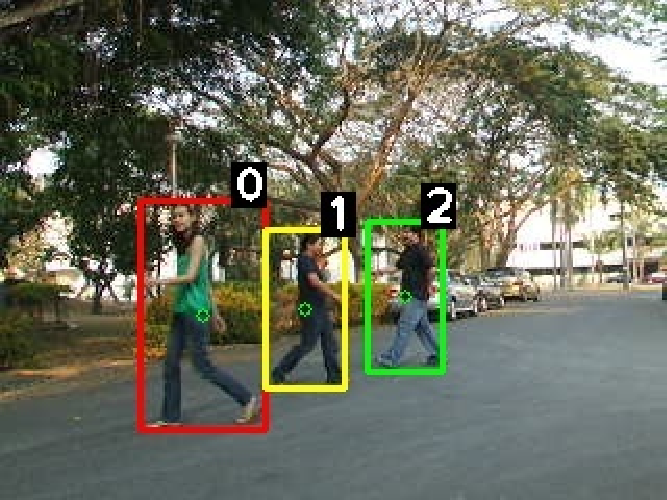
\includegraphics[scale=0.21]{figures/normal-tracking-result-0103.pdf} &
      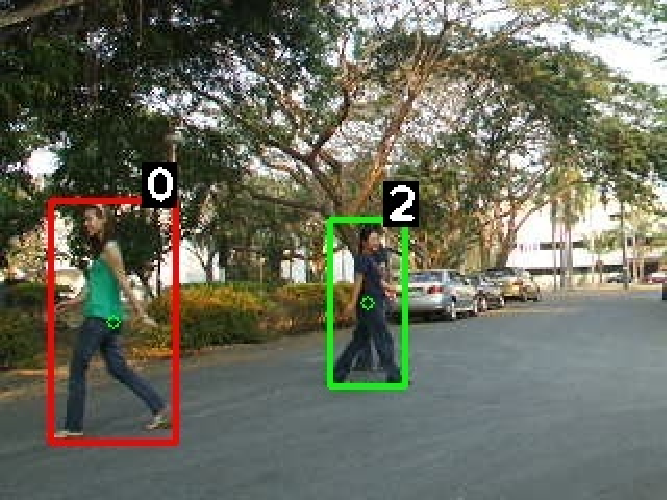
\includegraphics[scale=0.21]{figures/normal-tracking-result-0110.pdf} &
      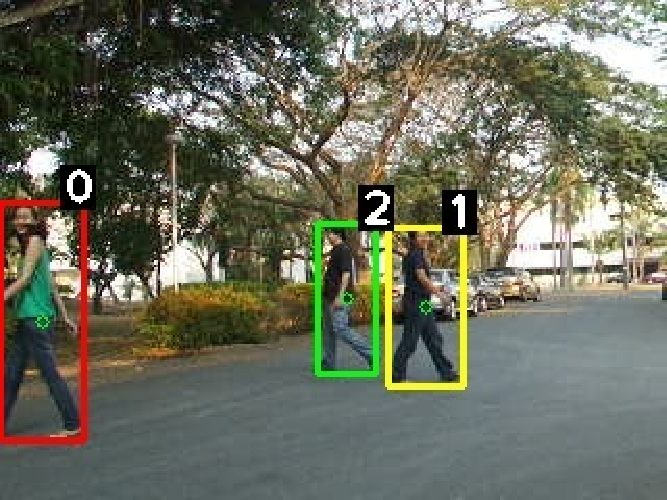
\includegraphics[scale=0.21]{figures/normal-tracking-result-0116.pdf} 
      \\
      \small Frame 90 & 
      \small Frame 94 & 
      \small Frame 103 & 
      \small Frame 110 & 
      \small Frame 116
    \end{tabular}
  \end{center}
  \caption[Sample blob tracking results for typical simple
    cases]{\small Sample blob tracking results for typical simple
    cases. In frame 94, track 0 and track 1 have merged.  In frame
    103, our method has correctly associated each motion blob with the
    correct track after they split. Similarly, frame 110 shows the
    result of another merge, and frame 116 shows the (correct) result
    when the merged motion blob splits.}
  \label{fig:normal-tracking-results}
\end{figure}

\begin{figure}[t]
  \begin{center}
    \begin{tabular}{ccccc}
      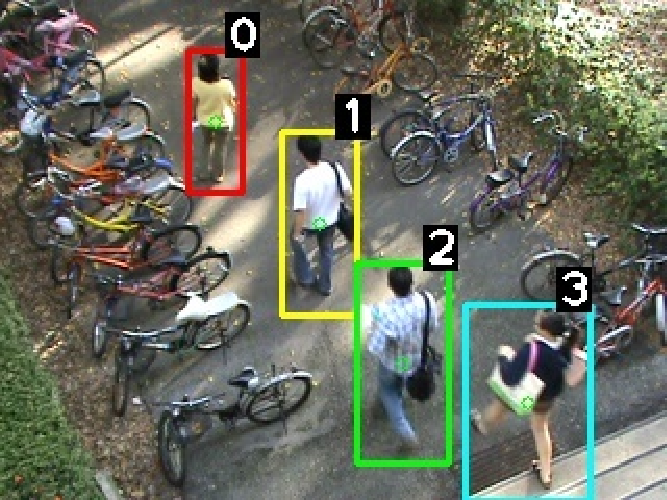
\includegraphics[scale=0.21]{figures/complex-tracking-result-0125.pdf} &
      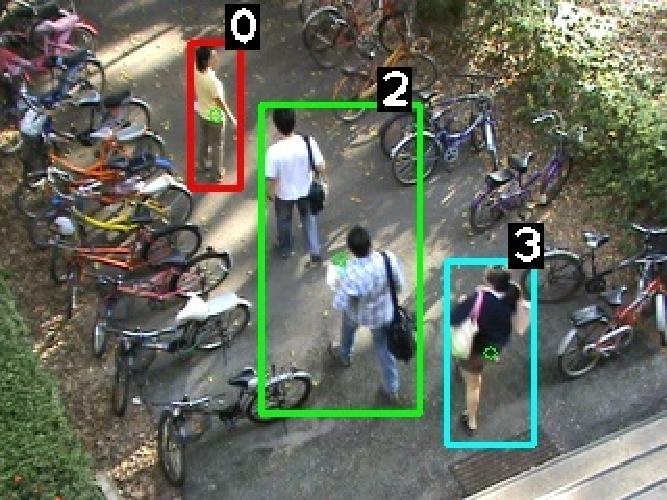
\includegraphics[scale=0.21]{figures/complex-tracking-result-0131.pdf} &
      \includegraphics[scale=0.21]{figures/complex-tracking-result-0133.pdf} &
      \includegraphics[scale=0.21]{figures/complex-tracking-result-0141.pdf} &
      \includegraphics[scale=0.21]{figures/complex-tracking-result-0160.pdf} 
      \\
      \small Frame 125 & 
      \small Frame 131 & 
      \small Frame 133 & 
      \small Frame 141 & 
      \small Frame 160
    \end{tabular}
  \end{center}
  \caption[Sample blob tracking results for a complex case.]{\small
    Sample blob tracking results for a complex case. In frame 131,
    track 1 and track 2 have merged. In frame 133, our method has
    correctly associated the current motion blobs with tracks after
    the merged blob splits. However, when the merged blob shown in
    frame 141 splits (in frame 160), we observe a track ID switch
    error in associating blobs with tracks.}
  \label{fig:complex-tracking-results}
\end{figure}

Once the blob-to-track association is performed, we represent each
track $i$ at time $t$ by a feature vector
\[
    \vec{f}_i^t = \begin{bmatrix} x_i^t & y_i^t & s_i^t & r_i^t &
        dx_i^t & dy_i^t & v_i^t \end{bmatrix},
\]
where $(x_i^t, y_i^t)$ is the centroid of the blob associated with
track $i$. $s_i^t$ is the area, in pixels, of the detected
blob. $r_i^t$ is the aspect ratio of the blob's bounding box,
calculated by dividing the width of the bounding box by its height.
$(dx_i^t, dy_i^t)$ is the unit motion vector for the blob associated
with track $i$ at time $t$ compared to track $i$ at time
$t-1$. $v_i^t$ is a temporally smoothed version of the speed of the
blob associated with track $i$, calculated as
\[
    v_i^t = r \frac{{\sqrt {(x_i^t - x_i^{t - 1} )^2 + (y_i^t - y_i^{t -
        1} )^2 } }}{{\Delta t}} + (1 - r) v_i^{t-1},
\]
where $r$ is a constant (we use $r=0.5$ in our experiments), $\Delta
t$ is the capture time difference between the frames at time $t$ and
$t-1$.

A preliminary report on the results for this appearance-based blob
tracking method appeared in \shortciteA{shashi10thesis}. \DIFdelbegin \DIFdel{The previous
}\DIFdelend \DIFaddbegin \DIFadd{I worked with
Gharti to produce the initial version of the method.  Since the
initial }\DIFaddend implementation was simplistic in some cases \DIFdelbegin \DIFdel{, }\DIFdelend and some work was
redundant\DIFdelbegin \DIFdel{. In the current work, I have }\DIFdelend \DIFaddbegin \DIFadd{, I }\DIFaddend improved the code to get better blob matching\DIFdelbegin \DIFdel{and }\DIFdelend \DIFaddbegin \DIFadd{.  
In particular, the current implementation does not need to create and 
label each group of merged tracks but use only the information gained 
from the merged track association matrix. I also }\DIFaddend eliminated unnecessary 
cases in the blob-to-track association process.

\DIFdelbegin \DIFdel{Although }\DIFdelend Kalman filtering or other methods may be more optimal for
filtering blob position and velocity over time, \DIFaddbegin \DIFadd{and tracking blobs 
with the filters could indeed improve the tracking results. 
In this dissertation, }\DIFaddend we find that they are unnecessary in 
practice because we observe relatively little noise in our \DIFdelbegin \DIFdel{data}\DIFdelend \DIFaddbegin \DIFadd{blob 
position from the tracker}\DIFaddend , and we map the feature vectors to discrete 
symbols fairly coarsely in the next step.

\section{Blob Feature Vector Discretization}
\label{sec:blob-discretization}

For simplicity, we use discrete-observation hidden Markov models (HMMs) 
in this dissertation. This means that each feature vector $\vec{f}_i^t$ must
be mapped to a discrete category (cluster ID) in the set $V = \{ v_1,
v_2, \ldots, v_U \}$, where $U$ is the number of categories. We use
$k$-means clustering based on a training set to map feature vectors to
discrete clusters.  Prior to clustering, we normalize each feature by
a $z$-score \DIFaddbegin \DIFadd{as in \ref{eq:z-score}.  
}\begin{equation}\DIFadd{
    \label{eq:z-score}
    z = \frac{x - \mu}{\sigma}
}\end{equation}
\DIFadd{where $\mu$ is the mean and $\sigma$ is the standard deviation of each 
feature}\DIFaddend . The scale factors are independent for all features
except $x_i^t$ and $y_i^t$, for which we apply a single isotropic
scale factor.

In the training stage, we run $k$-means with $U$ cluster centers then
save the cluster centers as a codebook for later use. We select $U$
based on the results of a model configuration selection procedure (to
be discussed in Section \ref{incremental-model-selection}). At run
time, each blob feature vector is mapped to the nearest cluster center
according to Euclidean distance then replaced by the corresponding
cluster ID. This means that a behavior sequence is finally represented
as a sequence of cluster IDs.

In the rest of this dissertation, when we mention the term
``observation sequence,'' we mean a sequence of cluster IDs. The
outputs to the next step are a list of blob feature vectors with the
corresponding cluster IDs and bounding boxes, and the current frame
and foreground mask.

\section{Discussion}
\label{sec:blob-discussion}

In this chapter, we segment each frame into background vs.\ foreground
and extract blobs with features using Poppe et al.'s improved mixture
of Gaussian background modeling method. We develop an appearance-based
method for blob tracking that uses the forward-backward overlap
technique and the color coherence vector (CCV) for occlusion handling.

The main limitation of our blob tracking method is that it is not
robust for complex events involving multiple people. The method also
does not allow evolution of the learned bootstrap model over time. 
Due to noise, fragmented blobs may affect the blob extraction, blob
feature extraction, and blob tracking results. An effective method to
handle blob fragmentation would be recommended for further
improvement.  In future work, we plan to address these limitations.

\FloatBarrier


%%% --- Maybe use later ---

%The limitations of the paper are that the system yields some errors
%when there are significant changes in lighting, and it also cannot
%distinguish between pedestrians moving at the same speed.

%The authors (Yamato) binarize the extracted image to calculate the mesh
%feature. Mesh features have been used as the low-level image features,
%and also have been successfully applied to complex 2D patterns such as
%multi-font characters \shortcite{umeda82font}. The calculation of mesh
%features is shown in Figure
%\ref{fig:mesh-feature}. The ratio of black pixels to total pixels in
%each mesh is an element of the feature vector.
%
%\begin{figure}[t]
%  \centering
%  \includegraphics[width=2in]{figures/mesh-feature.jpg}  
%  \caption[Mesh feature calculation]{Mesh feature
%    calculation. Reprinted from the work of Yamato et al.\ (1992).}
%  \label{fig:mesh-feature}
%\end{figure}

%In this paper, the authors (Nair and Clark) use the coordinates of
%the blob's center of mass, average color, and height to represent a
%blob.

%Although a lot of work has tried to improve the classic background
%modeling techniques, the fragmentation problem caused by a cluttered
%background still exist in blob detection and segmentation
%process. This problem is unavoidable in practice;
%therefore, \shortciteA{lu08segmentation} attempt to solve this problem
%and propose an effective connected components labeling method called
%connected chips linking (CCL). In this paper, they provide a function
%to calculate the correlation of space location between two blobs. Then
%they construct a correlation matrix based on the result. In order to
%handle fragmented blobs, they cluster the blobs using the information
%from the correlation matrix through the mean-shift algorithm. After
%that, they classify the blob-sets into ``Human'' or ``Fragments''
%using some criteria such as human
%size. Figure \ref{fig:blob-clustering-result} shows the result of
%handling fragmented blobs.
%
%\begin{figure}[t]
%  \centering
%  \subfloat[]{\includegraphics[scale=0.3]{figures/blob-clustering01.png}
%  \label{fig:blob-clustering01}}
%  \hspace{0.01in}
%  \subfloat[]{\includegraphics[scale=0.3]{figures/blob-clustering02.png}
%  \label{fig:blob-clustering02}}
%  \hspace{0.01in}
%  \subfloat[]{\includegraphics[scale=0.3]{figures/blob-clustering03.png}
%  \label{fig:blob-clustering03}}
%  \hspace{0.01in}
%  \subfloat[]{\includegraphics[scale=0.3]{figures/blob-clustering04.png}
%  \label{fig:blob-clustering04}}
%  \caption[Example of the result of handling fragmented
%  blobs.]{Example of the result of handling fragmented blobs. (a)
%  Background image. (b) Current image. (c) Foreground pixels. (d)
%  Result of handling fragmented blobs. Reprinted from the work of Lu
%  et al.\ (2008).}
%  \label{fig:blob-clustering-result}
%\end{figure}
%
%After segmenting the blob, the next step is to extract the blob
%features. \shortciteA{li06behavior} use the least median of squares
%(LMedS) method to construct the background model, then extract
%foreground by subtracting the background image. The authors propose a
%method based on space-time image features for automatic behavior
%modeling and recognition. This method is simple and insensitive to
%noise, and does not need to track parts of the human body. In this
%method, they extract the foreground, calculat shape features,
%represent the features as a space-time image. After the foreground is
%extracted, the authors equidistantly divide the bounded rectangle of
%the foreground into $10\times7$ sub-blocks. Then they normalized the
%value of each sub-block as follows:
%\[
%d_i = \left\lfloor {\frac{{s_i}}{{M}}\times255} \right\rfloor, i =
%  1,2, \ldots,k,
%\]
%where $k=10\times7$ is the number of sub-blocks; $s_i$ is the number
%of the foreground pixels in the $i^{th}$ sub-block; $M$ is the maximum
%value of $s_i$, where $i=1,2,...,k$. After that, they have the
%resulting shape descriptor $D_t$ at image frame $t$: $D_t =
%[d_1,d_2,d_3,...,d_k]$. Finally, to represent the motion of a sequence
%with $t$ frames, they construct the space time image representation
%(see Figure \ref{fig:space-time-feature}) as a matrix $I$ of size
%$t\times k$ as:
%\[
%I = [D_1,D_2,D_3,...,D_t]^{T}_{t\times k}
%\]
%They extract the features from this representation by Gabor filtering as 
%follows:
%\[
%F_n (x,y) = \iint {I_n (x_1 ,y_1 )G(x - x_1 ,y - y_1 ,f)dx_1dy_1},
%\]
%\[
%G(x,y,f) = \frac{1}{{2\pi \sigma _x \sigma _y }}\exp \left[ {
%- \frac{1}{2}\left( {\frac{{x^2 }}{{\sigma _x^2 }} + \frac{{y^2
%}}{{\sigma _y^2 }}} \right)} \right]M(x,y,f),
%\]
%\[
%M(x,y,f) = \cos \left[ {2\pi f(x\cos \theta + y\sin \theta)} \right],
%\]
%where $I_n(x,y)$ is the $n^{th}$ space-time image; $F_n(x,y)$ is the filtered 
%space-time image; the space constants of the Gaussian envelope along the $x$ 
%and $y$ axis are represented by $\delta _x$ and $\delta _y$, respectively; $f$ 
%is the frequency of the sinusoid and $\theta$ is the orientation of the Gabor 
%filter.
%
%\begin{figure}[t]
%  \centering
%  \includegraphics[width=1.5in]{figures/space-time-feature.jpg}
%  \caption[Space-time image representation]{Space-time image
%  representation. Reprinted from the work of Li et al.\ (2006)}
%  \label{fig:space-time-feature}
%\end{figure}
%
%There are some feature extraction methods that are able to capture
%motion history rather than having only current static
%features \shortcite{yamato92hmm,nair02surveillance}. One of them is
%motion history image (MHI) \shortcite{davis97mhi}. MHI is a static
%image template where pixel intensity is a function of the recency of
%motion in a video sequence. The idea is to represent how motion the
%image is moving. The MHI is defined as:
%\[
%  H_\tau  (x,y,t) = \left\{ \begin{array}{l}
%  \tau \quad \quad \quad \quad \quad \quad \quad \quad \quad \quad \quad \quad 
%  {\rm if}\;D(x,y,t) = 1 \\ 
%  \max (0,H_\tau  (x,y,t - 1) - 1)\quad {\rm otherwise}, \\ 
%  \end{array} \right.
%\]
%where $H_\tau (x,y,t)$ represents the MHI for a pixel $(x,y)$ at time
%$t$. The more recently moving pixels will be
%brighter. Figure \ref{fig:mhi} presents the examples of MHIs.
%
%\begin{figure}[t]
%  \centering
%  \includegraphics[width=4in]{figures/mhi}
%  \caption[Examples of motion history images]{Examples of motion
%  history images. Reprinted from the work of J. Davis \& Bobick
%  (1997).}
%  \label{fig:mhi}
%\end{figure}
%
%Based on the local intensity history of
%pixels, \shortciteA{xiang02event} proposed the pixel change history
%(PCH) to characterize pixel-wise temporal visual information in order
%to detect pixel-level events. The PCH is a representation of
%pixel-wise changes based on a combination of the pixel signal energy
%(PSE) proposed by \shortciteA{ng03pixel} and the MHI, which is
%computed as follows:
%\[
%  P_{\varsigma ,\tau } (x,y,t) = \left\{ \begin{array}{l}
%  \min (P_{\varsigma ,\tau } (x,y,t - 1) + \frac{{255}}{\varsigma },255)\quad 
%  \; {\rm if}\;D(x,y,t) = 1 \\ 
%  \max (P_{\varsigma ,\tau } (x,y,t - 1) + \frac{{255}}{\tau },0)\quad \quad 
%  {\rm otherwise}, \\ 
%  \end{array} \right.
%\]
%where $P_{\varsigma ,\tau } (x,y,t)$ represents the PCH for a pixel
%$(x,y)$ at time $t$, $D(x,y,t)$ indicates foreground regions at time
%$t$, $\varsigma$ is an accumulation factor, and $\tau$ is a decay
%factor. When the accumulation factor is set to 1, the PCH over the
%entire image is equivalent to the MHI. In this work, they did not
%specifically recognize human behaviors, but they proposed a new
%low-level primitive applicable to human representation that can
%describe human actions efficiently.
%
%Recursive filtering \shortcite{masoud03recognition} is a technique
%that encodes motion information such as the speed of the motion within
%a short period of time. The idea is to represent the ``recency'' of the
%motion. This technique is conceptually similar to the MHI. Let $I_t$
%be the frame at time $t$ and the filtered image $F_t$ at time $t$ is
%defined as follows:
%\[
%  F_t = \left| {I_t  - M_t } \right|
%\]
%\[
%  M_t = (1 - \beta)M_{t - 1}  + \beta M_t 
%\]
%\[
%  M_0 = I_0 = {\rm Background},
%\]
%where $t = 1, 2, \cdots, n_i$. If $\beta = 0$, the filtered image
%$F_t$ will be the foreground and if $\beta = 1$, $F_t$ will be
%equivalent to image differencing. Examples of filtered images are
%presented in \figurename~\ref{fig:f-img}.
%
%\begin{figure}[t]
%  \centering
%  \includegraphics[width=2.5in]{figures/f-img}
%  \caption[Examples of filtered images]{Examples of filtered
%  images. The coefficient $\beta$ is set to 0.5. Reprinted from the
%  work of Masoud \& Papanikolopoulos (2003).}
%  \label{fig:f-img}
%\end{figure}

\setlength{\footskip}{8mm}

\chapter{Extracting the Object from the Shadows: Maximum Likelihood
Object/Shadow Discrimination}
\label{ch:shadow}

\textit{In this chapter, we propose and experimentally evaluate a new
method for detecting shadows using a simple maximum likelihood
formulation based on color information. We first estimate, offline, a
joint probability distribution over the difference in the HSV color
space between pixels in the current frame and the corresponding pixels
in a background model, conditional on whether the pixel is an object
pixel or a shadow pixel.  Given the learned distribution, at run time,
we use the maximum likelihood principle to classify each foreground
pixel as either shadow or object.  In an experimental evaluation, we
find that the method outperforms standard methods on three different
real-world video surveillance data sets.  We conclude that the
proposed shadow detection method would be an extremely effective
component in an intelligent video surveillance system.}

\section{Introduction}

In many video surveillance applications, detecting and tracking moving
objects is an important issue. A \DIFdelbegin \DIFdel{very }\DIFdelend common approach to detect moving
objects is to apply background a subtraction algorithm. However,
background subtraction algorithms share one major disadvantage:
shadows tend to be misclassified as part of the foreground
object. This can lead to many undesirable consequences in the
detection step while segmenting and extracting features of moving
objects. For example, any estimate of the size of the detected object
would be an overestimate due to the misclassification of shadow pixels
as foreground pixels. Additionally, during object segmentation,
shadows misclassified as moving objects could lead to merging
otherwise separate blobs representing different people walking close
to each other.  This would make isolating and tracking people in a
group much more difficult than necessary.

Since shadow removal can significantly improve the performance of
computer vision tasks such as tracking, segmentation, and object
detection, shadow detection has become an active research area in
recent years.

Several well-known algorithms for shadow detection already exist. Most
of the work is based on background modeling and color difference
information. Generally, some model of the background is estimated,
then the difference between the background and current image is used
to identify changed pixels, then the changed pixels are further
classified into object and shadow.  Shadow pixels tend to have similar
chromaticity but lower luminance than the corresponding background
pixel.  In the RGB color space, chromaticity and luminance are not
orthogonal, but lighting differences can be controlled for in the
normalized RGB color space \shortcite{finlayson98colour}.  Some
research work thus utilizes the normalized RGB space in the background
subtraction and shadow removal
algorithm \shortcite{mckenna00tracking,elgammal02background,hong03background}.

\shortciteA{mikic00shadow} observe that in the normalized RGB color
space, shadow pixels tend to be more blue and less red than
illuminated pixels.  They apply a probabilistic model based on the
normalized red and blue features to classify shadow pixels in traffic
scenes. The authors assume that the background and shadow values
follow Gaussian distributions and foreground values follow a uniform
distribution. They iteratively estimate the posterior probabilities of
a given pixel belonging to each of three classes: background, shadow,
and foreground, until one of the probabilities reaches a fixed
threshold. The pixel is then classified accordingly.  If none of the
three probabilities reaches the threshold, the pixel is classified as
background.

\shortciteA{salvador04shadow} propose a new method for detecting
cast shadows. They first identify the presence of shadows in the RGB
color space based on the fact that shadows darken the surface they
cast on. The detected regions are further verified based on the color
invariance and geometric properties expected of shadows.

\shortciteA{havasi06geometric} illustrate that color-based methods
work well for weak shadows but not strong shadows. Hence, they
integrate geometric information into the detection process, resulting
in an iterative Bayesian framework combining both color and geometric
information that improves detection results.

One well-known problem with the normalized RGB space is that
normalization of pixels with low intensity results in unstable
chromatic
components \shortcite{kender76color}. \shortciteA{cucchiara01shadow}
and \shortciteA{chen08shadow} propose a HSV color-based method to
distinguish shadows from moving objects that eliminates this
concern. Their approach is based on the assumption that only the
intensity of the area covered by shadows will significantly
change. Therefore, they detect shadows using the so-called
deterministic nonmodel-based (DNM) approach as follows:
\[
  SP_t (x,y) = \left\{ 
  \begin{array}{ll}
    1 & {\rm if} \; \alpha \le \frac{{I_t^V (x,y)}}{{B_t^V (x,y)}} \le \beta\\ 
    & \;\;\; \wedge \; (I_t^S (x,y) - B_t^S (x,y)) \le T_S  \\ 
    & \;\;\; \wedge \left| {I_t^H (x,y) - B_t^H (x,y)} \right| \le T_H\\ \\
    0 & {\rm otherwise}, \\ 
  \end{array} \right.
\]
where $SP_t(x,y)$ is the resulting binary mask for shadows at each
pixel $(x,y)$ at time $t$.  $I_t^H$, $I_t^S$, $I_t^V$, $B_t^H$,
$B_t^S$, and $B_t^V$ are the H, S, and V components of foreground
pixel $I_t(x,y)$ and background pixel $B_t(x, y)$ at pixel $(x,y)$ at
time $t$, respectively.  They prevent foreground pixels from being
classified as shadow pixels by setting two thresholds, $0 < \alpha <
\beta < 1$.  The four thresholds $\alpha$, $\beta$, $T_S$, and $T_H$
are empirically determined.

Some researchers have investigated color spaces besides RGB and
HSV. \shortciteA{blau06shadow} use an ``improved'' hue, luminance, and
saturation (IHLS) color space for shadow detection to deal with the
issue of unstable hue at low saturation by modeling the relationship
between them. They then perform simple background subtraction method
based on the IHLS color space and saturation-weighted hue statistics.
Their experimental results show that detecting shadows in this color
is more reliable than in normalized RGB or HSV color spaces in several
video sequences.

Another alternative color space is YUV.  Some applications such as
television and videoconferencing use the YUV color space natively, and
since transformation from YUV to HSV is
time-consuming, \shortciteA{schreer02shadow} operate in the YUV color
space directly, developing a fast shadow detection algorithm based on
approximated changes of hue and saturation in the YUV color space.

There has been some work using texture-based methods such as the
normalized cross-correlation (NCC)
technique \shortcite{tian05shadow,jacques05shadow}. This method
detects shadows based on the assumption that the intensity of shadows
is proportional to the incident light, so shadow pixels should simply
be darker than the corresponding background pixels. Under this
assumption, shadow patches should be scaled versions of the
corresponding background patches. This assumption is most valid in
scenes with visible background texture inside the shadows. The method
computes the NCC between the neighborhood of a pixel in the foreground
mask and the neighborhood of the corresponding pixel in the background
model.  For each pixel $(i, j)$ of the foreground mask, it considers a
$(2N + 1)
\times (2N + 1)$ template $T_{ij}$ defined by $T_{ij}(n, m) = I(i+n,
j+m)$ for $-N \le n \le N$ and $-N \le m \le N$ ($N$ is empirically
determined). If $B(i, j)$ is the background model, the NCC value at
pixel $(i, j)$ is defined as follows:
\[
  NCC(i,j) = \frac{{ER(i,j)}}{{E_B (i,j)E_{T_{ij} } }},
\]
where
\[
  ER(i,j) = \sum\limits_{n = -N}^N {\sum\limits_{m = -N}^N {B(i + n,j
  + m)T_{ij} (n,m)}},
\]
\[
  E_B (i,j) = \sqrt {\sum\limits_{n = -N}^N {\sum\limits_{m = -N}^N
  {B(i + n,j + m)^2}}},
\]
\[
  E_{T_{ij} } = \sqrt {\sum\limits_{n = -N}^N {\sum\limits_{m = -N}^N
  {T_{ij} (n,m)^2}}}.
\]
For a pixel in a shadow region, the NCC value should be large (close
to one) and the $E_{T_{ij}}$ for the region around $(i,j)$, i.e., its
magnitude, should be smaller than $E_B (i,j)$. Consequently, a pixel
is classified as shadow if
\[
  NCC(i,j) \ge L_{NCC} 
\]
and
\[
  E_{T_{ij}} < E_B (i,j),
\]
where $L_{NCC}$ is an empirical threshold.

However, the texture-based method tends to misclassify foreground
pixels as shadow pixels when the foreground region has a similar
texture to the corresponding background
region. \shortciteA{xu05shadow} propose a hybrid shadow removal
technique that combines color and texture-based procedures to detect
shadows.  Since chromaticity in a shadow region should be the same as
the corresponding background region, and since the texture in a shadow
region should be the same as the corresponding background region, the
authors first classify pixels based on a set of thresholds for
brightness and color distortion then perform speckle removal filtering
to reconstruct the final foreground shapes.

Here we propose a new method for detecting shadows using maximum
likelihood estimation based on color information.  We extend the
deterministic nonmodel-based approach to parametric statistical
model-based approach. Our method estimates the joint distribution over
the difference in the HSV color space between pixels in the current
frame and the corresponding pixels in a background model, conditional
on whether the pixel is an object pixel or a shadow pixel. At run
time, we simply use the maximum likelihood principle to classify each
foreground pixel as either shadow or object given the estimated model.
Experimental results demonstrate that our proposed method outperforms
the standard methods (DNM and NCC) on three different real-world video
surveillance data sets. Our method is thus effective and also has the
potential to improve the object detection and motion analysis module
in intelligent video surveillance systems.

In the rest of this chapter, I provide details of the proposed method
and the overall process in Section \ref{sec:shadow-algorithm},
demonstrate the effectiveness of the shadow detection method with an
experimental evaluation in Section \ref{sec:shadow-results}, and then
conclude and point to future work in
Section \ref{sec:shadow-discussion}.

\section{Maximum Likelihood Classification of Foreground Pixels}
\label{sec:shadow-algorithm}

We divide our method into two phases.  In the first, offline phase, we
acquire training video, construct a background model from the first
few frames, perform foreground extraction on the remaining frames,
then manually label the extracted pixels as either object pixels or
shadow pixels.  I previously describe these steps in
Sections \ref{sec:blob-motion-detection}
and \ref{sec:blob-blob-extraction}. After that, we construct a joint
probability model over the difference in the HSV color space between
pixels in the current frame and the corresponding pixels in the
background model, conditional on whether the pixel is an object pixel
or a shadow pixel.

During the second, online phase, we perform the same background
modeling and foreground extraction procedure and further classify
foreground pixels as either shadow or object using the maximum
likelihood approach. I describe each of these steps in more detail in
the following sections.

\subsection{Offline Phase}

After foreground extraction, we manually label pixels as either shadow
or object. We then observe the distribution over the difference in hue
($H_{\text{diff}}$), saturation ($S_{\text{diff}}$), and value
($V_{\text{diff}}$) components in the HSV color space between pixels
in the current frame and the corresponding pixels in the background
model.  Figure \ref{fig:foreground-distribution} shows examples of
these distributions for object pixels, and
Figure \ref{fig:shadow-distribution} shows examples of these
distributions for shadow pixels.

\begin{figure}[t]
  \centering
  \subfloat[]{\includegraphics[scale=0.25]{figures/foreground_diff_h.png}}
  \hspace{0.05cm}
  \subfloat[]{\includegraphics[scale=0.25]{figures/foreground_diff_s.png}}
  \hspace{0.05cm}
  \subfloat[]{\includegraphics[scale=0.25]{figures/foreground_diff_v.png}}
  \caption[Example distributions over the difference in hue,
    saturation, and value components for true object pixels, extracted
    from our hallway dataset.]{\small Example distributions over the
    difference in (a) hue, (b) saturation, and (c) value components
    for true object pixels, extracted from our hallway dataset.}
  \label{fig:foreground-distribution}
\end{figure}

\begin{figure}[t]
  \centering
  \subfloat[]{\includegraphics[scale=0.25]{figures/shadow_diff_h.png}}
  \hspace{0.05in}
  \subfloat[]{\includegraphics[scale=0.25]{figures/shadow_diff_s.png}}
  \hspace{0.05in}
  \subfloat[]{\includegraphics[scale=0.25]{figures/shadow_diff_v.png}}
  \caption[Example distributions over the difference in hue,
    saturation, and value components for true shadow pixels, extracted
    from our hallway dataset.]{\small Example distributions over the
    difference in (a) hue, (b) saturation, and (c) value components
    for true shadow pixels, extracted from our hallway dataset.}
  \label{fig:shadow-distribution}
\end{figure}

Clearly, in all three cases, the distributions for object pixels and
shadow pixels are very different.  We thus introduce a measurement
probability distribution conditional on whether the assignment for a
pixel is object or shadow. In this work, we assume that the individual
component difference distributions are conditionally independent given
the assignment.

We define the \DIFdelbegin \DIFdel{measurement likelihood }\DIFdelend \DIFaddbegin \DIFadd{probability of measurement }\DIFaddend for pixel $(x, y)$ given its 
assignment as follows.
\begin{equation}
  \label{eq:shadow-measurement}
  \begin{array}{ccl}
    P(M_{\text{xy}} \mid A_{\text{xy}} = \text{sh}) 
            & = & P(H_{\text{diff}} \mid A_{\text{xy}} = \text{sh}) \times \\
            &   & P(S_{\text{diff}} \mid A_{\text{xy}} = \text{sh}) \times \\
            &   & P(V_{\text{diff}} \mid A_{\text{xy}} = \text{sh}),
  \end{array}
\end{equation}
where $M_{xy}$ is a tuple containing the HSV value for pixel $(x,y)$
in the current image as well as the HSV value for pixel $(x,y)$ in the
background model for pixel $(x,y)$, and $A_{xy}$ is the assignment of
pixel $(x,y)$ as object or shadow. ``sh'' stands for shadow.

\DIFdelbegin \DIFdel{To make the problem tractable, we }\DIFdelend \DIFaddbegin \DIFadd{We }\DIFaddend assume that the distributions over the components on the right 
hand side in \ref{eq:shadow-measurement} 
follow Gaussian distributions, defined as follows.
\begin{equation*}
  P(H_{\text{diff}} \mid A_{\text{xy}} = \text{sh}) =
  {\cal N}(H_{\text{diff}} ;
  \mu_{h_{\text{diff}}^{\text{sh}}},
  \sigma^2_{h_{\text{diff}}^{\text{sh}}})
\end{equation*}
\begin{equation*}
  P(S_{\text{diff}} \mid A_{\text{xy}} = \text{sh}) =
  {\cal N}(S_{\text{diff}} ;
  \mu_{s_{\text{diff}}^{\text{sh}}},
  \sigma^2_{s_{\text{diff}}^{\text{sh}}})
\end{equation*}
\begin{equation*}
  P(V_{\text{diff}} \mid A_{\text{xy}} = \text{sh}) =
  {\cal N}(V_{\text{diff}} ;
  \mu_{v_{\text{diff}}^{\text{sh}}},
  \sigma^2_{v_{\text{diff}}^{\text{sh}}})
\end{equation*}
\DIFaddbegin \DIFadd{Although the distributions for the true object pixels are clearly 
non-Gaussian as seen in Figure~\ref{fig:foreground-distribution}, 
I plan to extend this chapter in future work, but in 
this version, I simply use the sample mean and variance. However, 
on extension of the work, we will definitely investigate better 
estimators and different distributions.
}

\DIFaddend Similarly, the \DIFdelbegin \DIFdel{measurement likelihood }\DIFdelend \DIFaddbegin \DIFadd{probability of measurement given its assignment }\DIFaddend for 
object pixels can be computed as follows.
\begin{equation}
  \label{eq:foreground-measurement}
  \begin{array}{ccl}
    P(M_{\text{xy}} \mid A_{\text{xy}} = \text{obj}) 
            & = & P(H_{\text{diff}} \mid A_{\text{xy}} = \text{obj}) \times \\
            &   & P(S_{\text{diff}} \mid A_{\text{xy}} = \text{obj}) \times \\
            &   & P(V_{\text{diff}} \mid A_{\text{xy}} = \text{obj})
  \end{array}
\end{equation}
Here ``obj'' stands for object. As for the shadow pixel distributions,
we assume Gaussian distributions over the components on the right hand
side in \ref{eq:foreground-measurement}, as follows.
\begin{equation*}
  P(H_{\text{diff}} \mid A_{\text{xy}} = \text{obj}) =
  {\cal N}(H_{\text{diff}} ;
  \mu_{h_{\text{diff}}^{\text{obj}}},
  \sigma^2_{h_{\text{diff}}^{\text{obj}}})
\end{equation*}
\begin{equation*}
  P(S_{\text{diff}} \mid A_{\text{xy}} = \text{obj}) =
  {\cal N}(S_{\text{diff}} ;
  \mu_{s_{\text{diff}}^{\text{obj}}},
  \sigma^2_{s_{\text{diff}}^{\text{obj}}})
\end{equation*}
\begin{equation*}
  P(V_{\text{diff}} \mid A_{\text{xy}} = \text{obj}) =
  {\cal N}(V_{\text{diff}} ;
  \mu_{v_{\text{diff}}^{\text{obj}}},
  \sigma^2_{v_{\text{diff}}^{\text{obj}}})
\end{equation*}
We estimate the parameters $\Theta = \{
\mu_{h_{\text{diff}}^{\text{sh}}},
\sigma^2_{h_{\text{diff}}^{\text{sh}}},
\mu_{s_{\text{diff}}^{\text{sh}}},
\sigma^2_{s_{\text{diff}}^{\text{sh}}},
\mu_{v_{\text{diff}}^{\text{sh}}},
\sigma^2_{v_{\text{diff}}^{\text{sh}}},
\mu_{h_{\text{diff}}^{\text{obj}}},
\sigma^2_{h_{\text{diff}}^{\text{obj}}},
\mu_{s_{\text{diff}}^{\text{obj}}},
\sigma^2_{s_{\text{diff}}^{\text{obj}}},
\mu_{v_{\text{diff}}^{\text{obj}}},
\sigma^2_{v_{\text{diff}}^{\text{obj}}} \}$ directly from training
data during the offline phase.

\subsection{Online Phase}

Given the model estimate $\Theta$, we use the maximum likelihood
approach to classify a pixel as a shadow pixel if
\begin{equation}
  \label{eq:ml}
  P(M_{\text{xy}} \mid A_{xy}=\text{sh} ; \Theta ) >
  P(M_{\text{xy}} \mid A_{xy}=\text{obj} ; \Theta ).
\end{equation}
Otherwise, we classify the pixel as an object pixel.

We could add the prior probabilities to the shadow model and the
object model in \ref{eq:ml} to obtain a maximum a posteriori
classifier. In our experiments, we assume equal priors.

\section{Experimental Results}
\label{sec:shadow-results}

In this section, we present experimental results for our proposed
maximum likelihood (ML) classification method and compare the results
with two other methods from the literature, namely the deterministic
nonmodel-based (DNM)
method \shortcite{kender76color,cucchiara01shadow} and the normalized
cross-correlation (NCC)
method \shortcite{tian05shadow,jacques05shadow}.

\begin{figure}[t]
  \centering
  \subfloat[]{\includegraphics[scale=0.4]{figures/csim_hallway_benchmark.png}}
  \hspace{0.05cm}
  \subfloat[]{\includegraphics[scale=0.4]{figures/aton_lab_benchmark.png}}
  \hspace{0.05cm}
  \subfloat[]{\includegraphics[scale=0.4]{figures/aton_highway1_benchmark.png}}
  \caption[Sample frames from the Hallway, Laboratory, and Highway
    video sequences.]{\small Sample frames from the (a) Hallway, (b)
    Laboratory, and (c) Highway video sequences}
  \label{fig:benchmark}
\end{figure}

We performed the experiments on three video sequences.
Figure \ref{fig:benchmark} shows sample frames from the three video
sequences. The video sequences include both indoor and outdoor
scenes. The \textit{Hallway} sequence\footnote{Freely available for
others to experiment with
at: \url{http://www.kanouivirach.com/#downloads}.} shows a hallway
scene. For this video, we mounted a CCTV camera to record in an
academic building. The \textit{Laboratory} sequence shows a laboratory
room, and the \textit{Highway} sequence shows a traffic scene. The
last two video sequences were first introduced in Prati et al.'s
work\nocite{prati03shadow}.

To evaluate the performance of the methods, we compute the two metrics
proposed by \shortciteA{prati03shadow}, defining the shadow detection
rate $\eta$ and the shadow discrimination rate $\xi$ as follows:
\[
  \eta = \frac{TP_{\text{sh}}}{TP_{\text{sh}} + FN_{\text{sh}}};\; 
  \xi = \frac{TP_{\text{obj}}}{TP_{\text{obj}} + FN_{\text{obj}}},
\]
where the subscript ``sh'' and ``obj'' stand for shadow and object,
respectively. $TP$ and $FN$ are the number of true positive (i.e., the
shadow or object pixels correctly identified) and false negative
(i.e., the shadow or object pixels classified incorrectly) pixels.
$\eta$ expresses the proportion of shadow pixels correctly detected,
and $\xi$ expresses the proportion of object pixels correctly
detected.  $\eta$ and $\xi$ can also be thought of as the true
positive rate (sensitivity) and true negative rate (specificity) for
detecting shadows, respectively. In the experiment, we also compare
the methods with the additional two metrics: precision and $F_1$
score.

\subsection{Preparation}

Ground truth data are provided with the \textit{Laboratory} and
\textit{Highway} video sequences in Sanin et al.'s work\nocite{sanin12shadow}. 
They used a standard Gaussian mixture (GMM) background
model\nocite{stauffer99background} to extract foreground pixels for
the two videos. They selected 20 frames including objects from
the \textit{Laboratory} sequence arbitrarily for labeling.  For
the \textit{Highway} sequence, they labeled one out of every twenty
frames including objects for a total of 20 frames.  For our
\textit{Hallway} video sequence, to prepare similar ground truth data,
we selected one out of every ten frames including objects for 20
frames and manually labeled each pixel of each frame as object,
background, or shadow. We used the previously mentioned extended
version of the GMM background model for foreground extraction, but the
results were not substantially different from those of the standard
GMM.

To find the best parameters for each model while avoiding overfitting,
for each of the three models and each of the three data sets, we
performed five-fold cross validation using 10 of the training frames,
reserving the remaining 10 frames for the final test. The 10 frames in
each case were the second of every two frames in sequential order. We
varied the parameter settings for each method on each video dataset
and selected the setting that maximized the $F_1$ score (a measure
combining both precision and recall) over the cross validation test
sets. Finally, we tested on the remaining 10-frame final test set for
each video sequence.

\subsection{Shadow Detection Performance}

Table \ref{tab:comparison-results} compares the shadow detection
results between the proposed, DNM, and NCC methods.  Our method
achieves the top performance for shadow detection rate $\eta$ and
$F_1$ score in every case. We also obtain a good shadow discrimination
rate $\xi$ and precision in all three video
datasets. Figure \ref{fig:results-for-arbitrary-frame} shows the
results for an arbitrary frame in each video sequence. Green pixels
are those labeled as object pixels and red pixels are those labeled as
shadow pixels. The results in the figure confirm that our proposed
method clearly outperforms the two standard methods in all three video
datasets.

\begin{table}[t]
  \caption[Comparison of shadow detection results between the
    proposed, DNM, and NCC methods.]{\small Comparison of shadow
    detection results between the proposed, DNM, and NCC methods.}
  \begin{center}
    \includegraphics[width=6.1in]{figures/tab-shadow-results}
  \end{center}
  \label{tab:comparison-results}
\end{table}

\begin{figure}[t]
  \centering
  \includegraphics[width=6.2in]{figures/fig-shadow-results}
  \caption[Results for an arbitrary frame in each video
    sequence.]{\small Results for an arbitrary frame in each video
    sequence. The first column contains an example original frame for
    each video sequence. The second column shows the ground truth for
    that frame, where object pixels are labeled in white and shadow
    pixels are labeled in gray. The remaining columns show shadow
    detection results for each method, where pixels labeled as object
    shown in green and pixels labeled as shadow are shown in red.}
  \label{fig:results-for-arbitrary-frame}
\end{figure}

The DNM method has stable performance for all three videos, with good
performance for all metrics. Both the DNM method and our proposed
method suffer from the problem that the object colors can be confused
with the background color.  In the \textit{Highway} sequence (third
row in Figure \ref{fig:results-for-arbitrary-frame}), we clearly see
this situation. Our method detects shadows well but misclassifies some
object pixels as shadow, whereas DNM sometimes better discriminates
the shadow from the object.  However, the overall performance of our
proposed method is superior.

The NCC method achieves the best shadow discrimination rate $\xi$ and
precision. However, as can be seen in
Figure \ref{fig:results-for-arbitrary-frame}, this is because it
classifies nearly every pixel as object.  This gives NCC an advantage
for shadow precision and $\xi$ but on the other two metrics, shadow
detection rate $\eta$ and $F_1$ score, NCC performs extremely poorly
in all cases.  This is due to unclear background texture inside the
shadows, particularly on the \textit{Highway} sequence.

\section{Discussion}
\label{sec:shadow-discussion}

We propose a new method for detecting shadows using a simple maximum
likelihood approach based on color information.  We extend the
deterministic nonmodel-based approach, designing a parametric
statistical model-based approach. Our experimental results show that
our proposed method is extremely effective and superior to the
standard methods on three different real-world video surveillance data
sets.

In some cases, our method misdetects shadow pixels due to similar
color between the object and the background and unclear background
texture in shadow regions. Incorporating geometric or shadow region
shape priors would potentially improve the detection and
discrimination rates\DIFaddbegin \DIFadd{. 
}

\DIFadd{Additionally, the distributions over the difference 
in HSV color space for true object pixels and true shadow pixels remain 
static once trained. Therefore, the current approach may be inappropriate 
in the long run. More adaptive approach should be considered}\DIFaddend .

In future work, we plan to address these issues, further explore the
feasibility of combining our method with other useful shadow features,
and integrate our shadow detection module with a real-world open
source video surveillance system \shortcite{zoneminder}.

\FloatBarrier


%%% Old text %%%

%\section{Introduction}
%
%In video surveillance applications, moving object detection and
%tracking is an important issue.  A very common approach to detect
%moving objects is to apply a background subtraction technique. The
%process is basically to compare a new frame with a background
%model. The significant differences correspond to foreground. This
%process should ideally detect the moving objects and limit the false
%positive as much as possible at the same time.  More importantly, it
%should be able to avoid detection of shadows or noise. However, one
%challenging problem arising is to identify and detect shadows. And
%this has become an active research area in recent years.
%
%Shadows can cause lots of problems in the detection step while
%segmenting and extracting features of moving objects. For example, the
%size of detected object is larger than the real one due to the
%misclassification of shadow as foreground.  Shadows can also merge
%different people walking close to each other of which the output
%becomes a single object in the background subtraction step. Shadows
%and objects share two important information which make the problem
%difficult. Firstly, shadows can be detected as foreground because they
%are different from the background. Secondly, shadows have the same
%motion as the objects casting them.
%
%Generally, shadows can be categorized into two classes which are self
%and cast shadows. A self shadow occurs on the part of an object which
%is not illuminated by light. A cast shadow is an area projected where
%the light is occluded by an object. Figure \ref{fig:shadow-example}
%illustrates an example of self and cast shadow. One feature of shadows
%is that shadow does not significantly change the color and texture of
%the background, but only intensity. This feature is very useful since
%it can lead to many shadow detection algorithms which will be
%described in the next section.
%
%\begin{figure}[t]
%  \begin{center}
%  \includegraphics[width=2.5in]{figures/shadow-example.png}
%   \caption[Self and cast shadow in a real-world scene image]{Self and
%   cast shadow in a real-world scene image. Self shadow is on the back
%   of the person and cast shadow in on the ground.}
%  \label{fig:shadow-example}
%  \end{center}
%\end{figure}
%
%Removing shadows can significantly improve the performance of the
%computer vision tasks such as tracking, segmentation, and object
%detection. Since the detection and tracking is the core of video
%surveillance systems, poor detection and tracking can cause the
%problems to the next processing step such as feature extraction and
%behavior modeling. Background modeling techniques alone cannot solve
%the problems. We need an algorithm to detect and remove shadows.
%Therefore, in this dissertation, we explore and develop the shadow
%detection and removal algorithms. The experiments analyze the
%algorithms on the real-world video data.
%
%For the existing shadow detection
%methods, \shortciteA{cucchiara01shadow} and \shortciteA{chen08shadow}
%use the HSV color information to distinguish shadows from moving
%objects. Their approach is based on the assumption that only the
%intensity of the area covered by shadows will significantly change.
%Therefore, they can detect shadows using the following equation.
%\[
%  SP_t (x,y) = \left\{ \begin{array}{l}
%  1\;\;\;{\rm if}\;\alpha  \le \frac{{I_t^V (x,y)}}{{B_t^V (x,y)}} \le \beta\\ 
%  \quad \quad  \wedge (I_t^S (x,y) - B_t^S (x,y)) \le T_S  \\ 
%  \quad \quad  \wedge \left| {I_t^H (x,y) - B_t^H (x,y)} \right| \le T_H\\ \\
%  0\;\;\;{\rm otherwise}, \\ 
%  \end{array} \right.
%\]
%where $SP_t(x,y)$ is the binary mask of shadows at pixel $(x,y)$ at
%time $t$.  $I_t^H$, $I_t^S$, $I_t^V$, $B_t^H$, $B_t^S$, and $B_t^V$
%are H, S, V components of foreground pixel $I_t(x,y)$ and background
%pixel $B_t(x, y)$ at pixel $(x,y)$ at time $t$, respectively. They
%prevent the foreground pixel being classified into shadows by setting
%two thresholds $\alpha$ and $\beta$.  The parameter $\beta$ is set
%under 1 and $\alpha$ is set over 0. $T_S$ and $T_H$ are discovered by
%experiments.
%
%\shortciteA{tian05shadow}, \shortciteA{jacques05shadow},
%and \shortciteA{tan06shadow} apply the normalized cross-correlation
%(NCC) to detect shadows based on the assumption that the intensity of
%shadows is proportional to the incident light ,and shadow pixels are
%darker than background pixels, or it can be said that the shadows are
%the scaled versions of background. Therefore, using the NCC, they can
%identify the scaled versions of the same signal. They perform the NCC
%on the foreground mask from the background subtraction progress. For
%each pixel $(i, j)$ of the foreground mask, they considered a $(2N +
%1) \times (2N + 1)$ template $T_{ij}$, and defined $T_{ij}(n, m) =
%I(i+n, j+m)$ for $-N \le n \le N$, $-N \le m \le N$. $B(i,j)$ is the
%background image formed by temporal median filtering. The NCC at pixel
%$(x,y)$ is defined as.
%\[
%  NCC(i,j) = \frac{{ER(i,j)}}{{E_B (i,j)E_{T_{ij} } }},
%\]
%where
%\[
%  ER(i,j) = \sum\limits_{n = -N}^N {\sum\limits_{m = -N}^N {B(i + n,j
%  + m)T_{ij} (n,m)} },
%\]
%\[
%  E_B (i,j) = \sqrt {\sum\limits_{n = -qN}^N {\sum\limits_{m = -N}^N
%  {B(i + n,j + m)^2 } } },
%\]
%\[
%  E_{T_{ij} } = \sqrt {\sum\limits_{n = -N}^N {\sum\limits_{m = -N}^N
%  {T_{ij} (n,m)^2 } } }.
%\]
%For a pixel in a shadow region, the NCC value should be large (close
%to one) and the $E_{T_{ij}}$ of this region should be lower than the
%$E_B (i,j)$.  Consequently, a pixel is classified into shadow if
%\[
%  NCC(i,j) \ge L_{NCC} 
%\]
%and
%\[
%  E_{T_{ij} } < E_B (i,j),
%\]
%where $L_{NCC}$ is a threshold. Figure \ref{fig:tian-shadow-result}
%shows some examples of the results from the work
%of \shortciteA{tian05shadow}.
%
%\begin{figure}
%  \centering
%  \begin{tabular}{c}
%    \includegraphics[scale=0.7]{figures/tian-mog-results.png}\\
%    \includegraphics[scale=0.7]{figures/tian-shadow-results.png}
%  \end{tabular}
%  \caption[Examples of the background subtraction and shadow removal
%  results.]{Examples of the background subtraction and shadow removal
%  results. Upper row shows the results of the MoG background modeling
%  and lower row shows the results from the work of Tian et
%  al. Reprinted from the work of Tian et al.\ (2005).}
%  \label{fig:tian-shadow-result}
%\end{figure}
%
%Some authors found that the blue color component increases while the
%red color component decreases in a shadow
%region. \shortciteA{mikic00shadow} combine this information and
%normalized the blue and red color components as one of their
%features. After that, they apply a probabilistic model to classify
%shadow pixels in traffic scenes. They also assume that the background
%and shadow values follow a Gaussian distribution, and assume the
%foreground values follow an uniform distribution. They iteratively
%estimate the posterior probabilities of the pixel belonging to each
%of the three classes: background, shadow, and foreground until one of
%the probabilities reaches a fixed threshold. The pixel is then
%classified into one of those classes. If none of the three
%probabilities reaches the threshold, the pixel will be classified as
%background.
%
%\shortciteA{xu05shadow} assume that the chromaticity in a shadow
%region should be the same as when it is illuminated. Based on the
%information, they use a normalized chromatic color space to remove
%shadows. In this paper, they normalize the red and green color
%components. Then they define a set of thresholds for brightness and
%color distortion to classify a pixel value into foreground, highlight,
%or shadow.
%
%\shortciteA{hong03background} mention that there are both
%chromaticity and brightness in each pixel value in the RGB space. They
%remove the lightness by using the normalized RGB color space since the
%normalized RGB color space contains only the chromaticity. Thus, they
%use this information to propose their background subtraction
%approach. \shortciteA{havasi06geometric} illustrate that the color
%based method works well in case of weak shadow, but strong
%shadow. Hence, they integrate the geometric information into the
%detection process and came up with an iterative Bayesian framework
%which combines both the color and geometric information to improve the
%detection results.
%
%\section{Methodology}
%
%We use NCC and the maximum likelihood based on the HSV color
%information extracted from a set of training images to remove shadows.
%
%We compute the difference of hue $H_{\text{diff}}$, saturation
%$S_{\text{diff}}$, and value $V_{\text{diff}}$ components under the
%mask between the current and background frames. We simply calculate
%the probability as follows.
%
%\begin{equation*}
%  \begin{array}{ccl}
%    P(M_{\text{xy}} \mid A_{\text{xy}} = \text{sh}) 
%            & = & P(H_{\text{diff}}^{\text{sh}} \mid A_{\text{xy}} = \text{sh})
%                  P(S_{\text{diff}}^{\text{sh}} \mid A_{\text{xy}} = \text{sh}) \\
%            &   & P(V_{\text{diff}}^{\text{sh}} \mid A_{\text{xy}} = \text{sh}),
%  \end{array}
%\end{equation*}
%where $M_{xy}$ is a measurement at pixel $(x,y)$. To make the problem
%simple, we assume that the distribution of the difference of hue,
%saturation, and value components follows a normal distribution as
%follows.
%\begin{equation*}
%  P(H_{\text{diff}}^{\text{sh}} \mid A_{\text{xy}} = \text{sh}) \sim {\cal
%    N}(H_{\text{diff}}^{\text{sh}} ; 0, \sigma^2_{h_{\text{diff}}^{\text{sh}}}),
%\end{equation*}
%
%\begin{equation*}
%  P(S_{\text{diff}}^{\text{sh}} \mid A_{\text{xy}} = \text{sh}) \sim {\cal
%    N}(S_{\text{diff}}^{\text{sh}} ; 0, \sigma^2_{s_{\text{diff}}^{\text{sh}}}),
%\end{equation*}
%and
%\begin{equation*}
%  P(V_{\text{diff}}^{\text{sh}} \mid A_{\text{xy}} = \text{sh}) \sim {\cal
%    N}(V_{\text{diff}}^{\text{sh}} ; 0, \sigma^2_{v_{\text{diff}}^{\text{sh}}}).
%\end{equation*}
%
%\noindent Similarly, the measurement given the foreground assignment
%can be computed as follows.
%
%\begin{equation*}
%  \begin{array}{ccl}
%    P(M_{\text{xy}} \mid A_{\text{xy}} = \text{fg}) 
%            & = & P(H_{\text{diff}}^{\text{fg}} \mid A_{\text{xy}} = \text{fg})
%                  P(S_{\text{diff}}^{\text{fg}} \mid A_{\text{xy}} = \text{fg}) \\
%            &   & P(V_{\text{diff}}^{\text{fg}} \mid A_{\text{xy}} = \text{fg})
%  \end{array}
%\end{equation*}
%
%\noindent Each component is defined as follows.
%
%\begin{equation*}
%  P(H_{\text{diff}}^{\text{fg}} \mid A_{\text{xy}} = \text{fg}) \sim {\cal
%    N}(H_{\text{diff}}^{\text{fg}} ; 0, \sigma^2_{h_{\text{diff}}^{\text{fg}}}),
%\end{equation*}
%
%\begin{equation*}
%  P(S_{\text{diff}}^{\text{fg}} \mid A_{\text{xy}} = \text{fg}) \sim {\cal
%    N}(S_{\text{diff}}^{\text{fg}} ; 0, \sigma^2_{s_{\text{diff}}^{\text{fg}}}),
%\end{equation*}
%and
%\begin{equation*}
%  P(V_{\text{diff}}^{\text{fg}} \mid A_{\text{xy}} = \text{fg}) \sim {\cal
%    N}(V_{\text{diff}}^{\text{fg}} ; 0, \sigma^2_{v_{\text{diff}}^{\text{fg}}}).
%\end{equation*}
%
%Finally, we use the maximum likelihood approach to classify a pixel
%whether it is foreground or shadow.
%
%\section{Experimental Results}
%
%To collect data, we used ZoneMinder \shortcite{zoneminder} to capture
%video during two weeks. We set up a machine with a Web camera on the
%second floor in the Computer Science and Information Management (CSIM)
%building to capture activities in the scene.
%
%We have experimented with a shadow detection method using normalized
%cross correlation (NCC).  We compute the grayscale correlation between
%the foreground pixels and a background image constructed as the mean
%over each mixture of Gaussian distribution. Any foreground pixels
%whose NCC with the background are above some threshold
%$L_{\text{NCC}}$ are removed. In the experiments, we set
%$L_{\text{NCC}} = 0.995$. The results are shown in
%Figure \ref{fig:shadow-outdoor-result}. NCC works well in the outdoor
%scenes with visible background texture inside shadows. However, when
%we applied it in the indoor scenes, it does not work very well in many
%cases due to the lighting effect as shown in
%Figure \ref{fig:shadow-poor-result}.
%
%\begin{figure}[t]
%  \centering
%  \begin{tabular}{ccc}
%    \includegraphics[width=0.28\linewidth]{figures/shadow-result01.png} &
%    \includegraphics[width=0.28\linewidth]{figures/shadow-result02.png} &
%    \includegraphics[width=0.28\linewidth]{figures/shadow-result03.png}
%    \\
%    (a) & (b) & (c)
%    \end{tabular}
%  \caption{Sample foreground extraction and shadow removal results in
%    an outdoor scene.  (a) Original image. (b) Foreground pixels
%    according to background model.  (c) Foreground pixels after shadow
%    removal.}
%  \label{fig:shadow-outdoor-result}
%\end{figure}
%
%\begin{figure}[t]
%  \centering
%  \begin{tabular}{ccc}
%    \includegraphics[width=0.28\linewidth]{figures/shadow-poor-result01.png} &
%    \includegraphics[width=0.28\linewidth]{figures/shadow-poor-result02.png} &
%    \includegraphics[width=0.28\linewidth]{figures/shadow-poor-result03.png}
%    \\
%    (a) & (b) & (c)
%  \end{tabular}
%  \caption{Sample poor shadow removal results in an indoor scene.  (a)
%    Original image. (b) Foreground pixels according to background
%    model.  (c) Foreground pixels after shadow removal. Red pixels
%    show the positives, and green pixels show the negatives.}
%  \label{fig:shadow-poor-result}
%\end{figure}
%
%We have performed another experiment using a maximum likelihood
%approach on the HSV color space. We first compute the difference of
%hue, saturation, and value under the mask of the current and
%background frames from a set of training images. The distributions of
%those values under the foreground mask are shown in
%Figure \ref{fig:foreground-distribution}, and the distributions under
%the shadow mask are shown in Figure
%\ref{fig:shadow-distribution}. For the hue and saturation values, we
%subtracted the current frame by the background frame, but for the
%intensity value, to get the positive values, we subtracted the
%background frame by the current frame.
%
%\begin{figure}[t]
%  \centering
%  \subfloat[]{\includegraphics[width=0.32\linewidth]{figures/foreground_diff_h.png}}
%  \hspace{0.05in}
%  \subfloat[]{\includegraphics[width=0.32\linewidth]{figures/foreground_diff_s.png}}
%  \hspace{0.05in}
%  \subfloat[]{\includegraphics[width=0.32\linewidth]{figures/foreground_diff_v.png}}
%  \caption{Distribution of the difference of hue, saturation, and
%    value under the foreground mask. (a) Difference of hue.(b)
%    Difference of saturation. (c) Difference of value.}
%  \label{fig:foreground-distribution}
%\end{figure}
%
%\begin{figure}[t]
%  \centering
%  \subfloat[]{\includegraphics[width=0.32\linewidth]{figures/shadow_diff_h.png}}
%  \hspace{0.05in}
%  \subfloat[]{\includegraphics[width=0.32\linewidth]{figures/shadow_diff_s.png}}
%  \hspace{0.05in}
%  \subfloat[]{\includegraphics[width=0.32\linewidth]{figures/shadow_diff_v.png}}
%  \caption{Distribution of the difference of hue, saturation, and
%    value under the shadow mask. (a) Difference of hue. (b) Difference
%    of saturation. (c) Difference of value.}
%  \label{fig:shadow-distribution}
%\end{figure}
%
%The results for the maximum likelihood approach compared to the NCC
%approach are shown in Figure \ref{fig:comparison-shadow-results}.
%
%\begin{figure}[t]
%  \centering
%  \begin{tabular}{cccc}
%    \includegraphics[width=0.22\linewidth]{figures/shadow-original.png} &
%    \includegraphics[width=0.22\linewidth]{figures/shadow-bg-results.png} &
%    \includegraphics[width=0.22\linewidth]{figures/shadow-ncc-results.png} &
%    \includegraphics[width=0.22\linewidth]{figures/shadow-ml-results.png}
%    \\
%    (a) & (b) & (c) & (d)
%    \end{tabular}
%  \caption{Shadow removal results in an indoor scene.  (a) Original
%    image. (b) Foreground pixels according to background model. (c)
%    Shadow detection using NCC.  (d) Shadow detection using the
%    maximum likelihood approach.}
%  \label{fig:comparison-shadow-results}
%\end{figure}
%









\setlength{\footskip}{8mm}

\chapter{Clustering Human Behaviors with Dynamic Time 
Warping and Hidden Markov Models}
\label{ch:clustering}

\textit{In this chapter, we propose and experimentally evaluate a new 
method for clustering human behaviors that is suitable for
bootstrapping an anomaly detection module for intelligent video
surveillance systems. The method uses dynamic time warping,
agglomerative hierarchical clustering, and hidden Markov models to
provide an initial partitioning of a set of observation sequences then
automatically identifies where to cut off the hierarchical clustering
dendrogram. We show that the method is extremely effective, providing
100\% accuracy in separating anomalous from typical behaviors on
real-world testbed video surveillance data.}

\section{Introduction}
\label{sec:clustering-intro}

Human behavior understanding is an important component of a wide
variety of desirable intelligent systems.  However, the problem is
very difficult, due to the wide range of activities possible in any
given context and the large amount of variability within any
particular activity. Many researchers have attempted to build systems
able to interpret and understand human behaviors. The most classic
work is from \shortciteA{yamato92hmm}, who model
tennis actions using hidden Markov models (HMMs). 
\shortciteA{du06activity} present an approach to recognize
interaction activities using dynamic Bayesian networks (DBNs) that
outperforms conventional HMMs. \shortciteA{gao04dining}
use a single mixture-of-Gaussian HMM, in which the states represent
the stages of dining activities, to monitor the eating behavior of
elderly people in a nursing home.

As video monitoring is becoming more ubiquitous in our lives, research
on advanced video surveillance analysis is increasingly important.  To
help security personnel work reliably and efficiently, we would like
to filter out typical events, and in cases of anomalous events,
automatically raise an alarm or present the event to a human operator
for consideration as a security threat. Most existing work assumes
that the number of ``normal'' behavior patterns need to be known
beforehand. For example, \shortciteA{nair02surveillance} built an
automated video surveillance system using HMMs, each modeling a
common, predefined activity in a scene.

In more recent years, research has started to focus on unsupervised
analysis and clustering of behaviors in a particular scene for a
variety of purposes including anomaly detection, surveillance, and
classification. \shortciteA{zhong04detection} treat video segments as
documents and cluster the documents based on the co-occurrence
information. \shortciteA{li06behavior} cluster human gestures by
constructing an affinity matrix using dynamic time warping (DTW;
Sakoe, 1978)\nocite{sakoe78dtw} then apply the normalized-cut approach
to cluster the gestures. \shortciteA{hautamaki08clustering} apply DTW
and use the pairwise DTW distances as input to a hierarchical
clustering process in which $k$-means is used to fine-tune the output.

Here we use a combination of clustering and HMMs to group
human behaviors in a scene. There is some recent related work using
graphical models such as HMMs to cluster behavior
patterns. \shortciteA{li99pattern} use the Bayesian information
criterion (BIC) for HMM model selection and construct a binary
hierarchical clustering dendrogram to initialize data partitions based
on a sequence-to-model likelihood distance measure. They then compare
each pair of clusters using a partition mutual information (PMI)
criterion \shortcite{bahl86speech} to find the optimal number of
clusters.

\shortciteA{xiang05profiling} model the distribution of
activity data in a scene using a Gaussian mixture model (GMM) and also
employ the BIC to select the optimal number of behavior classes prior
to HMM training.

\shortciteA{swears08clustering} propose hierarchical HMM-based clustering
to find and cluster motion trajectories and velocities in a highway
interchange scene. They build up a set of HMMs incrementally. For each
new trajectory, they first test the likelihood of the trajectory
according to each existing HMM model.  If the new observation is not
fit by any existing model, it is considered deviant and is grouped
with other deviant observations to form a new HMM.

\shortciteA{alon03clustering} propose a method to discover groupings of
similar object motions. They apply a finite mixture of HMMs where the
number of mixture components is assumed to be known. They estimate the
number of clusters using the minimum description length (MDL)
criterion \shortcite{rissanen98mdl}, a penalized likelihood measure.

In this dissertation, we propose a new method for clustering human
behaviors in the context of video surveillance.  After extracting
sequences of features representing individual human behaviors in a
given scene, we use DTW to measure the pairwise similarity between
sequences. Then we construct an agglomerative hierarchical clustering
dendrogram based on the DTW similarity measure. To find the optimal
set of behavior clusters, we start at the root of the tree, train a
HMM on the patterns in that cluster, and determine how well the HMM
models the set of patterns in the cluster.  When we find that a HMM is
an insufficient representation of the patterns in a given cluster, we
throw away that HMM and recursively consider each of the child
clusters according to the pre-calculated DTW-based dendrogram. Our
method is able to automatically find the common human behaviors
occurring in a given scene. In an experiment with a testbed video
surveillance data set, we find that the method separates typical
behaviors and abnormal behaviors into separate sets of clusters with
100\% accuracy.

The most similar related work is that
of \shortciteA{oates01clustering}, who first proposed the idea of
using the DTW with HMMs to cluster time series. They use the DTW
dendrogram cut off at an arbitrary depth as an initial partition of
the training sequences, then they train HMMs on each partition
iteratively until they have a set of HMMs that models all of the
training sequences.  They apply their method to simulated time series
with good results but report obtaining poor clustering results in an
experiment with real robot sensor data.

As we shall see in later chapters, the method improves upon the state
of the art in intelligent video surveillance applications by
bootstrapping human behavior classification and anomaly detection
modules in a given installation. Once a set of initial clusters and
corresponding HMMs representing typical behavior is determined, we can
easily find which cluster a new sequence should fall into by
performing statistical tests on the sequence's likelihood according to
each HMM model.  When the likelihood is low according to all of the
pre-existing clusters, we can consider the sequence to be anomalous
and alert a human operator. When the likelihood is sufficiently high
for one of the pre-existing models, we can simply incrementally update
the sufficient statistics for that model.  This approach would allow
raising alerts for behaviors inconsistent with the
automatically-derived typical behavior profile for the scene while
providing adaptation to gradual changes in typical behavior patterns
over time. We do not focus on these incremental learning and anomaly
detection issues in this chapter. We consider these issues in later
chapters.

In the rest of this chapter, I provide the details of our human
behavior clustering algorithm in
Section \ref{sec:clustering-algorithm}, demonstrate the feasibility of
the algorithm with an experimental evaluation in
Section \ref{sec:clustering-results}, and then conclude and point to
future work in Section \ref{sec:clustering-discussion}.

\section{Human Behavior Pattern Clustering}
\label{sec:clustering-algorithm}

\subsection{Overview}

\begin{figure}[t]
  \centering
  \subfloat[]{\includegraphics[scale=0.4]{figures/blob-extraction-block-diagram}
  \label{fig:overview-blob}}
  \subfloat[]{\includegraphics[scale=0.4]{figures/behavior-clustering-block-diagram}
  \label{fig:overview-clustering}}
  \caption[Block diagrams for the proposed method.]{\small Block
    diagrams for the proposed method.  (a) Blob extraction flow. (b)
    Behavior clustering flow.}
  \label{fig:overview-blob-diagram}
\end{figure}

Figure \ref{fig:overview-blob-diagram} provides an overview of the
architecture of our proposed method.  The blob extraction phase
(Figure \ref{fig:overview-blob}) generates observation sequences from
videos as follows:

\begin{enumerate}
  \item Grab a few initial frames from an the input video to model the
    background scene.
  \item Perform foreground extraction to get a list of blobs.
  \item Find the single largest blob in the scene, remove any pixels
    likely to be shadow pixels, and extract feature vector $\vec{f}_t$
    for the blob at time $t$. \DIFaddbegin \DIFadd{In this chapter, for simplicity, we 
    evaluate our method only with a single moving blob.
  }\DIFaddend \item Apply vector quantization using the $k$-means algorithm to
    convert features into symbols.
  \item Aggregate symbol sequences and store for batch cluster
    analysis.
\end{enumerate}

In the behavior clustering phase
(Figure \ref{fig:overview-clustering}), for the set of all discrete
symbol sequences, we perform the following steps:

\begin{enumerate}
  \item Apply DTW to the set of sequences to construct a
    similarity-based distance matrix.
  \item Run agglomerative hierarchical clustering on the distance
    matrix to get a dendrogram.
  \item Perform HMM-based hierarchical clustering using the set of
    sequences and the dendrogram to get a set of HMMs modeling the
    typical behaviors in the scene.
\end{enumerate}

\subsection{Blob Extraction}
\label{sec:clustering-blob-extraction}

Here we use the motion detection and blob extraction methods
previously described in Sections \ref{sec:blob-motion-detection}
and \ref{sec:blob-blob-extraction}, respectively.

In the work reported in this chapter, we use a simple normalized cross
correlation (NCC) shadow elimination method described in
Chapter \ref{ch:shadow} to eliminate shadows cast by moving objects.
We compute the grayscale correlation between the foreground pixels and
a background image constructed as the mean over each mixture of
Gaussian distribution. Any foreground pixels whose NCC with the
background are above some threshold are removed. We choose this method
because it works well in outdoor scenes where background texture
inside shadows is visible.  The sample results from the foreground
extraction and shadow removal procedures are shown in
Figure \ref{fig:shadow-result}. We use the NCC method for shadow
removal through the rest of this dissertation.

\begin{figure}
  \centering
  \subfloat[]{\includegraphics[width=0.28\linewidth]{figures/shadow-result01.png}
  \label{fig:shadow-result-original}}
  \hspace{0.1in}
  \subfloat[]{\includegraphics[width=0.28\linewidth]{figures/shadow-result02.png}}
  \hspace{0.1in}
  \subfloat[]{\includegraphics[width=0.28\linewidth]{figures/shadow-result03.png}}
  \caption[Sample foreground extraction and shadow removal
    results.]{\small Sample foreground extraction and shadow removal
    results.  (a) Original image. (b) Foreground pixels according to
    background model. (c) Foreground pixels after shadow removal.}
  \label{fig:shadow-result}
\end{figure}

We next apply morphological opening and closing operations \DIFaddbegin \DIFadd{by probing 
an image with a disk structure element of radius 5 }\DIFaddend to remove
noise and connect foreground regions\DIFdelbegin \DIFdel{, then we }\DIFdelend \DIFaddbegin \DIFadd{. The opening operation of a binary 
image $A$ by the predefined structuring element $B$ is obtained by the 
erosion of $A$ by $B$, followed by dilation of the 
resulting image by $B$, which is defined as 
}\begin{equation*}\DIFadd{
    A \circ B = (A \ominus B) \oplus B, 
}\end{equation*}
\DIFadd{The closing operation is of $A$ and $B$ is obtained by the dilation of 
$A$ by $B$, followed by erosion of the resulting structure by $B$, 
which is defined as 
}\begin{equation*}\DIFadd{
    A \bullet B = (A \oplus B) \ominus B.
}\end{equation*}

\DIFadd{We then }\DIFaddend obtain the connected
foreground components (blobs) and filter out any components whose size
is below threshold. In this \DIFdelbegin \DIFdel{work}\DIFdelend \DIFaddbegin \DIFadd{chapter}\DIFaddend , for simplicity, we evaluate our
clustering method with videos containing a single moving blob. \DIFaddbegin \DIFadd{We have 
extended the algorithm to handle multiple moving blobs in next chapters.
}\DIFaddend 

We therefore follow the process previously described in
Section \ref{sec:blob-appearance-based-blob-tracking} for representing
a blob (connected foreground component) by a feature vector,
normalizing each feature independently, and quantizing the feature
vectors into discrete symbols using $k$-means.

%We therefore simply represent a blob (connected foreground component)
%at time $t$ by the feature vector
%\[
%  \vec{f}_t = \begin{bmatrix} x_t & y_t & s_t & r_t & dx_t & dy_t &
%  v_t \end{bmatrix},
%\]
%where $(x_t,y_t)$ is the centroid of the blob, $s_t$ is the size of
%the blob in pixels, $r_t$ is the aspect ratio of the blob's bounding
%box, $(dx_t,dy_t)$ is the unit-normalized motion vector for the blob
%compared to the previous frame, and $v_t$ is the blob's speed compared
%to the previous frame, measured as
%\[
%  v_t = \frac{{\sqrt {(x_t - x_{t - 1} )^2 + (y_t - y_{t - 1} )^2 }
%  }}{{\Delta t}},
%\]
%where $\Delta t$ is the capture time difference between the frames at
%time $t$ and $t-1$. We increase the stability by using an average
%velocity, measured as
%\[
%  v_t  = rv_t  + (1 - r)v_{t - 1},
%\]
%where $r$ is a constant. We use $r=0.5$ in our experiments.

%After extracting the feature vectors $\vec{f}_t$ over a training set,
%we quantize them into discrete symbols using $k$-means. To prevent
%differing numeric scales of the features from affecting the distance
%metric, we normalize each feature independently by $z$-scaling to a
%mean of 0 and standard deviation of 1 over the training set.  For the
%vectors $(x_t,y_t)$ and $(dx_t,dy_t)$, rather than normalize the $x$
%and $y$ components independently, we use a common isotropic scale
%factor for the two dimensions to avoid overemphasizing small
%deviations from typical trajectories in directions without much
%deviation in the training data.

Currently, we empirically tune the free parameters (frame buffer
length, thresholds, and number of $k$-means clusters) to the training
data. We hope to automate the blob extraction parameter selection
process in future work.

\subsection{Behavior Clustering}
\label{sec:clustering-behavior-clustering}

We model the common behaviors in a scene by clustering a set of
observation sequences acquired over some period of time. First, we
apply dynamic time warping (DTW) to estimate the similarity between
every pair of training sequences despite variations in length and
speed, to obtain a similarity matrix. Second, we use the similarity
matrix for hierarchical agglomerative clustering by first combining
the most similar two sequences into a single cluster then repeatedly
merging clusters until just one cluster is left at the root of the
tree or dendrogram.  To determine the similarity of two clusters
during this step, we use the similarity of the most similar pair of
sequences between the two clusters.

The resulting DTW dendrogram provides a convenient representation of
the similarity structure within a set of time sequences, but
hierarchical clustering always comes with the practical issue of
determining the optimal cutoff or number of clusters to use in a
particular application.  We solve this problem using HMMs as described
below.

The flow of the algorithm is summarized in
Figure \ref{fig:flow-diagram}.  We begin at the root of the
hierarchical clustering dendrogram and attempt to model the sequences
in that cluster (all training sequences, for the root) using a
HMM. When there are more than $N$ sequences in parent cluster $c$
whose per-observation log likelihood is less than a threshold $p_c$,
we consider the HMM to be inadequate, throw it away, and then
recursively attempt to model each of $c$'s children in the DTW
dendrogram.  We use $N=10$ in our experiments. The per-observation log
\DIFdelbegin \DIFdel{likelihood of }\DIFdelend \DIFaddbegin \DIFadd{of the probability of }\DIFaddend a sequence $\vec{O}_i = \{ O_{i, 1}, O_{i, 2} \cdots
O_{i, T_i} \}$ \DIFdelbegin \DIFdel{is
}\[\DIFdel{
  L_{i} = \frac{\log P( \vec{O}_i \mid M_c )}{T_i},
}\]
%DIFAUXCMD
\DIFdelend \DIFaddbegin \DIFadd{given the HMM $M_c$ is
}\begin{equation}\DIFadd{
    L_{i} = \frac{\log P( \vec{O}_i \mid M_c )}{T_i},
}\end{equation}
\DIFaddend where $M_c$ is the HMM that models the sequences in cluster $c$, $T_i$
is the number of observations in sequence $i$, and $P(\vec{O}_i
\mid M_c)$ is calculated using the forward algorithm \shortcite{rabiner89hmm}.

%(calculated using the forward algorithm; Rabiner,
%1989\nocite{rabiner89hmm})

\begin{figure}[t]
  \begin{center} \includegraphics[width=3.8in]{figures/clustering-flow-diagram} \end{center} \caption[Processing
    flow of the use of HMM clustering method.]{\small Processing flow
    of the use of HMM clustering method.}  \label{fig:flow-diagram}
\end{figure}

To determine the optimal rejection threshold $p_c$ for cluster $c$, we
use an approach similar to that of \shortciteA{oates01clustering}.  We
generate random sequences from the HMM and then calculate the mean
$\mu_c$ and standard deviation $\sigma_c$ of the per-observation log
likelihood over the set of generated sequences.  For the lengths of
the generated sequences, we simply use the average length of the
training patterns in cluster $c$.  After obtaining the statistics of
the per-observation log likelihood, we let $p_c$ be $\mu_c -
z \sigma_c$, where $z$ is an experimentally tuned parameter that gives
us convenient control over the probability of making Type I errors in
classifying a particular sequence as having been generated by a
particular HMM model.

\section{Experimental Results}
\label{sec:clustering-results}

To create a testbed data set, we mounted a CCTV camera to view the
scene in front of an academic building, as seen in
Figure \ref{fig:shadow-result-original}. We recorded videos at a
resolution of $320 \times 240$ and 25 frames per second over one week
during working hours (9:00--17:00). To save disk space, we used a
motion detection technique that automatically segments a raw video
stream into separate videos containing motion. We obtained videos
corresponding to over 500 motion events then manually selected the 298
videos containing only a single motion.

We found that there are at least four common behaviors in this scene:
people walking into the building, walking out of the building, parking
a bicycle, and riding a bicycle out. Figure \ref{fig:example-behavior}
shows examples of each of these behaviors. Other less common
activities include people walking into the scene then walking out or
people walking while telephoning and leaving the scene. For purposes
of evaluating the results of our algorithm, we hand-labeled each of
the videos with the categories Walk-in, Walk-out, Cycle-in, Cycle-out,
or Other.

\begin{figure}[t]
  \centering
  \subfloat[]{\includegraphics[width=0.2\linewidth]{figures/example-behavior01.pdf}}
  \hspace{0.05in}
  \subfloat[]{\includegraphics[width=0.2\linewidth]{figures/example-behavior02.pdf}}
  \hspace{0.05in}
  \subfloat[]{\includegraphics[width=0.2\linewidth]{figures/example-behavior03.pdf}}
  \hspace{0.05in}
  \subfloat[]{\includegraphics[width=0.2\linewidth]{figures/example-behavior04.pdf}}
  \caption[Examples of common human activities in our testbed
    scene.]{\small Examples of common human activities in our testbed
    scene.  (a) Walking in. (b) Walking out.  (c) Cycling in. (d)
    Cycling out.}
  \label{fig:example-behavior}
\end{figure}

We performed three experiments to evaluate our method. In Experiment
I, we applied our proposed method, as previously described, to cluster
the 298 single-motion videos in our testbed data set. In Experiment
II, we used an alternative clustering method that only uses recursive
modeling by HMMs, without DTW. In Experiment III, we used an
alternative method combining HMMs with supervised learning. In every
experiment, we evaluated the clustering results (or classification
results in the case of the supervised system of Experiment III)
according to how well the induced categories separate the anomalous
sequences (hand-labeled with the category ``Other'') from the typical
sequences (Walk-in, Walk-out, Cycle-in, Cycle-out). Our main
hypothesis was that \textit{using DTW as a pre-process prior to
HMM-based clustering should improve the quality of the clusters} in
terms of separating anomalous from typical behaviors. One might also
have hypothesized that supervised learning (Experiment III) would be
better than either of the unsupervised methods (Experiments I and II),
but as we shall see, we obtained a somewhat surprising result to the
contrary.

In all three experiments, we used linear HMMs with four states and
bypass transitions. That is, each HMM had transitions from state 1 to
states 1, 2, and 3, from state 2 to states 2, 3, and 4, from state 3
to states 3 and 4, and from state 4 to itself. We chose this model
structure based on our previous empirical
experience \shortcite{kan08thesis}.

To find the distribution (parameters $\mu_c$ and $\sigma_c$) of the
per-observation log likelihood for a particular HMM, we always
generated 1000 sequences of 120 observations then used a $z$-threshold
of 2.0, corresponding to a Type I error (probability of misclassifying
a sequence generated by the HMM as not generated by the HMM) of
0.0228.  We fixed the parameter $N$ (the number of deviant patterns
allowed in a cluster) to 10.

\subsection{Experiment I (DTW+HMMs)}

\begin{table}[t]
  \caption[Clustering results for Experiment I (DTW+HMMs).]{\small
    Clustering results for Experiment I (DTW+HMMs).}
  \label{tab:dtw-and-hmm-assoc-matrix}
  \begin{center}
    \begin{tabular}{c|c|c|c|c|c}
      \hline
      Cluster \# & Walk-in & Walk-out & Cycle-in & Cycle-out & Other \\ 
      \hline \hline
      1  & 96 & 0  & 18 & 0 & 0 \\ \hline
      2  & 0  & 54 & 0  & 5 & 0 \\ \hline
      3  & 0  & 3  & 0  & 8 & 0 \\ \hline
      4  & 0  & 2  & 0  & 0 & 0 \\ \hline
      5  & 0  & 1  & 0  & 2 & 0 \\ \hline
      6  & 0  & 0  & 0  & 2 & 0 \\ \hline
      7  & 0  & 0  & 0  & 2 & 0 \\ \hline
      8  & 0  & 0  & 0  & 2 & 0 \\ \hline
      9  & 0  & 0  & 0  & 2 & 0 \\ \hline
      10 & 0  & 0  & 2  & 0 & 0 \\ \hline
      11 & 0  & 0  & 2  & 0 & 0 \\ \hline
      12 & 0  & 0  & 3  & 0 & 0 \\ \hline
      13 & 0  & 0  & 1  & 1 & 0 \\ \hline
      14 & 0  & 0  & 0  & 0 & 4 \\ \hline
      15 & 0  & 0  & 0  & 0 & 4 \\ \hline
      16 & 0  & 0  & 0  & 0 & 2 \\ \hline
      17 & 0  & 0  & 0  & 0 & 2 \\ \hline
      One-seq clusters & 4 & 17 & 34 & 21 & 4 \\ \hline
    \end{tabular}
  \end{center}
\end{table}

The clustering results are shown in
Table \ref{tab:dtw-and-hmm-assoc-matrix}. The method obtained 97
clusters. For the 17 clusters containing more than one sequence, we
show the distribution of the activities represented by each
sequence. For the 80 clusters containing only a single sequence, we
summarize their distribution across the activity categories in the
last row of the table.

It is clear from the results that the separation of anomalous and
typical behaviors is excellent (100\% accuracy), with the caveat that
80 sequences (26.8\% of the data set) fall into single-sequence
clusters that would have to be manually examined by a human operator
if the method was used to bootstrap a real-world surveillance system.

\DIFaddbegin \DIFadd{It is worth pointing out that since the current system treats each 
($z$-scaled) feature equally when it performs blob feature vector 
discretization, important fine distinctions for some features can be 
lost. Adding more weight to features such as blob size or aspect ratio 
could help distinguish the similar behaviors such as the Walking In 
and Cycling In behaviors. 
}

\DIFaddend \subsection{Experiment II (HMMs only)}

To determine the extent to which our system benefits from
preprocessing using DTW, in this experiment, we used the concept of
recursive modeling of the data using HMMs without using DTW as a
pre-process.  The method is similar to that
of \shortciteA{swears08clustering}.  We begin by training a single HMM
on all sequences and computing the distribution of the per-observation
log likelihood for that HMM as previously described.  We then assign
every sequence with a per-observation log likelihood above threshold
$p_c$ to a cluster then repeat the process by training a new HMM on
the remaining sequences.  Similarly to the method of Experiment I, we
stop splitting whenever the number of deviant sequences in the cluster
is less than 10.

\begin{table}[t]
  \caption[Clustering results for Experiment II (HMMs only).]{\small
    Clustering results for Experiment II (HMMs only).}
  \label{tab:hmm-assoc-matrix}
  \begin{center}
    \begin{tabular}{c|c|c|c|c|c}
      \hline
      Cluster \# & Walk-in & Walk-out & Cycle-in & Cycle-out & Other \\ 
      \hline \hline
      1 & 15 & 77 & 49 & 43 & 16 \\ \hline
      2 & 80 & 0 & 11 & 2 & 0 \\ \hline	
      3 & 5 & 0 & 0 & 0 & 0 \\ \hline	
    \end{tabular}
  \end{center}
\end{table}

The results are shown in Table \ref{tab:hmm-assoc-matrix}. The method
obtains only three clusters, and the clusters are incapable of
separating anomalous behaviors from typical behaviors.  With manual
assignment of all three clusters to the ``typical'' category, we would
achieve a recall of 0, a precision of 100\%, and an accuracy of
94.6\%.  By manually assigning cluster 1 to the anomalous category, we
would achieve a recall of 100\%, a precision of 8\%, and an accuracy
of 38.3\%.  These strikingly poor results confirm our main hypothesis,
and we conclude that recursive HMM modeling without DTW-based
preprocessing is useless for video surveillance.

\subsection{Experiment III (Supervised classification with HMMs)} 

As an alternative approach to \DIFdelbegin \DIFdel{separating }\DIFdelend \DIFaddbegin \DIFadd{separate }\DIFaddend anomalous from typical
behaviors, in this experiment, we trained four HMMs on 80\% of each of
the four typical behaviors observed in our testbed data set.  We
retained 20\% of each typical sequences and the 16 anomalous sequences
as a test set. After HMM training, we manually determined the best
per-observation log likelihood threshold for each HMM by maximizing
the F1 value (a measure combining both precision and recall) for the
separation between the positive and negative test patterns.  The
anomalous pattern detection rate of the the combined classifier was
50\% (8 patterns) with a false alarm rate of 24.6\% (16 out of 65
normal testing patterns).

A priori, one might have hypothesized that supervised sequence
classification should outperform the unsupervised method we have
proposed in this chapter.  To the contrary, we find that the
simple-minded approach of training a single HMM on each typical
behavior is far inferior.  Clearly, there is more variation within the
behavior categories than can be handled precisely by single simple
HMMs.  These supervised results could presumably be improved by
applying our clustering method within each behavior category, thus
obtaining a collection of HMMs for each behavior category.  However,
we have already demonstrated that our method achieves perfect
separation of anomalous and typical behaviors \textit{without any
information about the labels}, so this approach would be unnecessarily
laborious.

\section{Discussion}
\label{sec:clustering-discussion}

In this chapter, we have proposed and evaluated a new method for
clustering human behaviors.  As we shall see, the method can be used
to bootstrap an anomaly detection module for intelligent video
surveillance systems.  The combination of DTW partitioning with linear
HMM training turns out to be quite powerful; manual examination of the
clusters obtained from our method shows a perfect separation between
typical and anomalous behaviors on a real-world testbed video
surveillance data set.

The combination of DTW with the type of linear HMMs we use in this
work is surprisingly effective. It is likely that the patterns DTW
groups together are perfectly suited for modeling by this type of HMM.
We plan to further explore this idea in future work.

There are two key limitations to our current method. The first is that
we limited the data to single motion events. The remaining chapters
will eliminate that constraint. The second is that although the method
achieves 100\% accuracy in separating typical from anomalous events,
it does so at the cost of creating a fairly large number of
single-sequence clusters that would have to be manually identified as
typical or anomalous by a human operator in a real surveillance
setting.

\FloatBarrier


\setlength{\footskip}{8mm}

\chapter{Automatic Suspicious Behavior Detection from 
a Small Bootstrap Set}
\label{ch:batch}

\textit{In this chapter, we propose and evaluate a new method for 
automatic identification of suspicious behavior in video surveillance
data. The approach works by constructing scene-specific statistical
models explaining the behaviors occurring in a small bootstrap data
set. It partitions the bootstrap set into clusters then assigns new
observation sequences to clusters based on statistical tests of HMM
log likelihood scores. Cluster-specific likelihood thresholds are
learned rather than set arbitrarily.  In an evaluation on a real-world
testbed video surveillance data set, the method proves extremely
effective, with a false alarm rate of 7.4\% at a 100\% hit rate. The
method is thus a practical and effective solution to the problem of
inducing scene-specific statistical models useful for bringing
suspicious behavior to the attention of human security personnel.}

\section{Introduction}
\label{sec:batch-intro}

Video surveillance is ubiquitous in our lives, but the ongoing
proliferation of surveillance cameras makes it increasingly difficult
to monitor all channels continuously. As the amount of surveillance
video increases, monitoring becomes more expensive and less
effective. Security would be enhanced if it were possible to perform
intelligent filtering of typical events and to automatically bring
suspicious events to the attention of human security personnel.

The goal of automated suspicious event detection, however, requires
some level of human behavior understanding. Many researchers have
attempted to build intelligent systems able to interpret and
understand human
behaviors \shortcite{davis98activity,masoud03recognition,cao04motion,sminchisescu05motion,du06activity,li06behavior,wang06gesture}.
Pre-trained hidden Markov models (HMMs) and other dynamic Bayesian
networks such as conditional random fields (CRFs) have been widely
used in this area, ranging from visual activity
recognition \shortcite{yamato92hmm,sminchisescu05motion,xiang05profiling,vail07activity},
gesture recognition \shortcite{wilson00gesture,gao04dining}, and
unusual activity
detection \shortcite{nair02surveillance,lee03modeling,chan04event,wu05behavior,andrade06crowd,snoek06event,zhang05event,arsic07behavior}. However,
the problem is difficult and remains unsolved, due to the wide range
of activities possible in any given context and the large amount of
variability within any particular activity. In the context of video
surveillance, the problem is even more challenging because behavior
considered normal in one scene might be considered unusual in another
scene.

%Most existing work creates separate models for each distinct a priori
%known class of normal behavior. One example is the work
%of \shortciteA{nair02surveillance}, which performs automated video
%surveillance using HMMs, each modeling a common, pre-defined activity
%in a scene. They classify a sequence as anomalous if the log
%likelihood of the sequence is below a pre-defined threshold for all
%trained HMMs. Other
%work \shortcite{arsic07behavior,lee03modeling,wu05behavior} uses
%support vector machines (SVMs) to model and classify behaviors into
%pre-defined classes.

Here we propose a method for automatic suspicious behavior detection
that utilizes a small bootstrap set in which observation sequences are
manually labeled as normal or suspicious (warranting an operator's
attention).  Using the algorithm from Chapter~\ref{ch:clustering}, we
partition the bootstrap set into clusters of similar sequences and
model each cluster with a simple HMM. We then label each behavior
cluster as normal or possibly suspicious based on the labels of the
individual sequences mapped to the cluster.

After bootstrapping is complete, we assign new observation sequences
to behavior clusters using statistical tests on the log likelihood of
the sequence according to the corresponding HMMs.  A sequence is
considered suspicious if the most likely cluster is already labeled as
suspicious or if its log likelihood according to the most likely
cluster's HMM is too low.  The cluster-specific likelihood threshold
is learned rather than set arbitrarily.

In an evaluation on a real-world video surveillance situation, we find
that, based on a bootstrap set of 150 human motion sequences, our
method is extremely effective at identifying suspicious behavior, with
a false positive rate of 7.4\% at a hit rate of 100\%.  The proposed
method dramatically outperforms traditional machine learning
approaches using the same bootstrap set for training.

Our method is thus a practical and effective solution to the problem
of inducing scene-specific statistical models useful for bringing
suspicious behavior to the attention of human security personnel.

In the rest of this paper, we provide the details of our human
behavior modeling and bootstrapping algorithm in
Section \ref{sec:batch-modeling} and our anomaly detection method in
Section \ref{sec:batch-anomaly-detection}. We demonstrate the feasibility
of the algorithm with an experimental evaluation in
Section \ref{sec:batch-results}, and then discuss and point to future
work in Section \ref{sec:batch-discussion}.

\section{Behavior Model Bootstrapping}
\label{sec:batch-modeling}

Our method for bootstrapping a model of the specific behaviors in a
scene is a batch procedure based on a training video stream acquired
over a short period of time such as one week.  We first perform moving
blob tracking on the training video on the assumption that moving
blobs of sufficient size are people or groups of people.  For each
blob, we extract a sequence of feature vectors describing the blob's
trajectory and appearance over time.  From these data, we
automatically bootstrap a bank of linear HMMs, each model specializing
in one type of behavior.

\begin{figure}[t]
  \centering
  \includegraphics[width=1\linewidth]{figures/behavior-modeling-block-diagram}
  \caption[Block diagram of our overall system.]{\small Block diagram
    of our overall system.}
  \label{fig:behavior-modeling-block-diagram}
\end{figure}

Here we follow the processing steps for motion detection described in
Section \ref{sec:blob-motion-detection} and blob extraction described
in Section \ref{sec:blob-blob-extraction}. 

We define an ``event'' as a contiguous change or motion detected over
some period of time. Extremely short events (occasionally occurring
due to noise) are automatically removed before processing.

Next we use the tracking algorithm previously described in
Section \ref{sec:blob-appearance-based-blob-tracking} to track the
obtained blobs, extract a sequence of feature vectors describing each
blob's trajectory and appearance over time, and automatically
bootstrap a bank of linear HMMs, each model specializing in one type
of behavior.

However, one difference between this chapter and the previous chapter
is that this chapter extends the simple single blob tracking method to
the full multiple blob tracking method described in
Chapter~\ref{ch:blobanalysis}.

\subsection{Behavior Clustering}
\label{sec:batch-behavior-clustering}

After blob tracking, we obtain, from a given video, a set of
observation sequences describing the motion and appearance of every
distinguishable moving object in the scene.  We next partition the
observation sequences into clusters of similar behaviors then model
the sequences within each cluster using a simple linear HMM. 

In this section, we use the method previously described in
Chapter~\ref{ch:clustering}, which first uses dynamic time warping
(DTW) to obtain a distance matrix for the set of observation sequences
then performs agglomerative hierarchical clustering on the distance
matrix to obtain a dendrogram (a binary tree expressing the similarity
structure within the set of observation sequences).  To determine
where to cut off the dendrogram, we traverse the DTW dendrogram in
depth-first order from the root and attempt to model the observation
sequences within the corresponding subtree using a single linear HMM.
If, after training, the HMM is unable to ``explain'' (in the sense
described below) the sequences associated with the current subtree, we
discard the HMM then recursively attempt to model each of the current
node's children. Whenever the HMM is able to explain the observation
sequences associated with the current node's subtree, we retain the
HMM and prune the tree.

A HMM is said to explain or model a cluster $c$ of observation
sequences if there are no more than $N_c$ sequences in $c$ whose
per-observation log-likelihood is less than a threshold $p_c$.  We use
$N_c=10$ in our experiments. The per-observation log likelihood of a
sequence is previously defined in
Section~\ref{sec:clustering-behavior-clustering}.

To determine the optimal rejection threshold $p_c$ for cluster $c$, we
use an approach similar to that of \shortciteA{oates01clustering}. We
generate random sequences from the HMM and then calculate the mean
$\mu_c$ and standard deviation $\sigma_c$ of the per-observation log
likelihood over the set of generated sequences.  For the lengths of
the generated sequences, we simply use the average length of the
sequences in the bootstrap set.  After obtaining the statistics of the
per-observation log likelihood, we let $p_c$ be $\mu_c - z \sigma_c$,
where $z$ is an experimentally tuned parameter that gives us
convenient control over the probability of making Type I errors in
classifying a particular sequence as having been generated by a
particular HMM model.

Our method solves the problem by educing an initial partitioning of
the human behavior observation sequences into groups based on
similarity. Once the set of all behaviors has been partitioned into
groups containing similar sequences, as we shall see, each group can
be modeled individually with a simple statistical model, the linear
HMM. Next, we can use the resulting bank of trained models for anomaly
detection.

The clustering process results in a set of $K$ different typical
behavior clusters ${\cal C} = \{ C_1, C_2, \ldots, C_K \}$ with a set
of $K$ corresponding HMMs ${\cal M} = \{ M_1, M_2, \ldots, M_K \}$.

\section{Anomaly Detection}
\label{sec:batch-anomaly-detection}

In this section we describe our method for anomalous or suspicious
behavior detection. In the \textit{supervised} approach, one would
construct a training set consisting of anomalous and normal behaviors,
build a model, then use the model to classify new behavior sequences
as anomalous or normal.

The pure supervised approach is obviously not suitable, however, when
examples of anomalous behavior are sparse or nonexistent.  In
practical scenarios, the set of possible anomalous behaviors is
infinite in its variety, making it very difficult to acquire a
representative training set.

In the \textit{unsupervised} approach, on the other hand, we would
simply construct a generative model of the normal behavior patterns,
then use the model to classify new behavior sequences as abnormal when
they are ``too far'' in some sense from typical behavior.  For
example, we could use the algorithm described in
Section \ref{sec:batch-behavior-clustering} to construct a bank of
HMMs explaining the normal sequences in a training set of patterns,
then classify new sequences as abnormal or suspicious whenever the
likelihood of the sequence according to the most likely HMM is below
some specific threshold.

The difficulty with the pure unsupervised approach, however, is that
there is no clear way to calibrate the parameters of the ``too far''
criterion.  In practice, one would have to select a conservative
initial distance threshold then fine-tune the threshold to achieve the
best tradeoff between hit and false positive rates.  An inappropriate
initial cutoff could lead to disastrous misses of suspicious behavior
or inundation with false positives.

Since both approaches have limitations, rather than the pure
supervised method or the pure unsupervised method, we instead propose
a \textit{semi-supervised} method that self-calibrates itself from a
small bootstrap set in which each bootstrap sequence is manually
labeled as normal or suspicious by a human operator.  Our method is
simple.  We acquire labels for the bootstrap patterns from the
operator, then we apply the algorithm of
Section \ref{sec:batch-behavior-clustering} to
\textit{both the positive and negative sequences} in the bootstrap
set.  We identify each cluster as a ``normal'' cluster if \textit{all}
of the sequences falling into it are labeled as normal, or identify it
as an ``abnormal'' cluster if \textit{any} of the sequences falling
into it are labeled as abnormal.

For the time complexity of this method, in principle, if we updated
the log likelihood for each model every time we receive a new
observation in constant time, the time complexity would be O($nm$),
where $n$ is the number of observations and $m$ is the number of
models. However, for convenience, we rerun the forward
algorithm \shortcite{rabiner89hmm} on each observation for every
model.

Algorithm \ref{anomaly-detection-algorithm} is a pseudocode summary of
the runtime anomaly detection method. New sequences are classified as
normal if the most likely HMM for the input sequence is associated
with a cluster of normal sequences \textit{and} the $z$-scaled
per-observation log \DIFdelbegin \DIFdel{likelihood of the }\DIFdelend \DIFaddbegin \DIFadd{of the probability of the }\DIFaddend sequence under that most likely
model is greater than a global empirically determined threshold
$\theta_z$.

\begin{algorithm}[t]
  \caption{Anomaly Detection}
  \label{anomaly-detection-algorithm}
  \begin{algorithmic}
    \REQUIRE $\vec{O}$: behavior sequence
    \REQUIRE ${\cal M}$: set of HMMs
    \STATE ${\cal M}_{ab} \gets \{ M \mid M \in {\cal M} \text{~and $M$ is marked abnormal} \}$
    \STATE $( M_{ml}, L_{ml} ) \gets \textsc{Find-Most-Likely-Model}(\vec{O}, {\cal M})$
    \IF{$M_{ml} \in {\cal M}_{ab}$ or $L_{ml} \leq \theta_z$}
      \STATE $\textsc{Alert-Security-Personnel}(\vec{O})$
    \ENDIF
  \end{algorithmic}
\end{algorithm}

\section{Experimental Results}
\label{sec:batch-results}

We created a testbed data set using a CCTV camera with a view of the
front of a building, as seen in
Figure \ref{fig:batch-example-behavior}(a). Videos were recorded at 25
frames per second with a resolution of $320 \times 240$ during working
hours (9:00--17:00) for two weeks. We used the previously-described
techniques to segment the raw video stream into separate videos
containing motion, track blobs, extract features, discretize the
feature vectors, and create observation sequences. We obtained 423
video segments containing 660 observation sequences.

We observed that there are four common activities in this scene:
people walking into the building, people walking out of the building,
people parking bicycles, \DIFdelbegin \DIFdel{and }\DIFdelend people riding bicycles out\DIFaddbegin \DIFadd{, and people walking 
pass by or having interactions with each other}\DIFaddend . 
Figure \ref{fig:batch-example-behavior} shows examples of 
each of these behaviors. In our experiments, we considered all other 
behaviors, such as walking around looking for an unlocked bicycle, to 
be suspicious or abnormal. 

\begin{figure}[t]
  \centering
  \DIFdelbeginFL %DIFDELCMD < \subfloat[]{\includegraphics[width=0.2\textwidth]{figures/example-behavior01.pdf}\label{fig:example-of-scene}}
%DIFDELCMD <   %%%
\DIFdelFL{\hspace{0.05in}
  }%DIFDELCMD < \subfloat[]{\includegraphics[width=0.2\textwidth]{figures/example-behavior02.pdf}}
%DIFDELCMD <   %%%
\DIFdelFL{\hspace{0.05in}
  }%DIFDELCMD < \subfloat[]{\includegraphics[width=0.2\textwidth]{figures/example-behavior03.pdf}}
%DIFDELCMD <   %%%
\DIFdelFL{\hspace{0.05in}
  }%DIFDELCMD < \subfloat[]{\includegraphics[width=0.2\textwidth]{figures/example-behavior04.pdf}}
%DIFDELCMD <   %%%
\DIFdelendFL \DIFaddbeginFL \subfloat[]{\includegraphics[width=0.19\textwidth]{figures/example-behavior01.pdf}\label{fig:example-of-scene}}
  \DIFaddFL{\hspace{0.03in}
  }\subfloat[]{\includegraphics[width=0.19\textwidth]{figures/example-behavior02.pdf}}
  \DIFaddFL{\hspace{0.03in}
  }\subfloat[]{\includegraphics[width=0.19\textwidth]{figures/example-behavior03.pdf}}
  \DIFaddFL{\hspace{0.03in}
  }\subfloat[]{\includegraphics[width=0.19\textwidth]{figures/example-behavior04.pdf}}
  \DIFaddFL{\hspace{0.03in}
  }\subfloat[]{\includegraphics[width=0.19\textwidth]{figures/example-behavior05.pdf}}
  \DIFaddendFL \caption[Examples of common human activities in our testbed
    scene.]{\small Examples of common human activities in our testbed scene.
    (a) Walking in. (b) Walking out. (c) Cycling in. (d) Cycling out. 
    \DIFaddbeginFL \DIFaddFL{(e) Other group activities.}\DIFaddendFL }
  \label{fig:batch-example-behavior}
\end{figure}

To evaluate the effectiveness of our method, we divide the experiments
into two parts: model configuration selection (finding an optimal set
of HMMs to model the bootstrap set) and anomaly detection based on the
HMM bootstrap set. In all of the experiments, we used linear HMMs. We
chose this model structure based on our previous empirical
experience \shortcite{kan08thesis}.

\subsection{Model Configuration Selection}
\label{sec:batch-model-config}

We first manually labeled each of the videos with the categories
``normal'' or ``abnormal.''  For purposes of analyzing the results, we
further subdivided the normal patterns into categories ``walk-in,''
``walk-out,'' ``cycle-in,'' and ``cycle-out,'' but we did not use
these labels for model selection or learning.

Towards model identification, we then performed a series of
experiments with different bootstrap parameter settings and selected
the configuration with the highest accuracy in separating the normal
sequences from the abnormal sequences on the bootstrap sequence set,
as measured by the false positive rate for abnormal sequences.  (Every
bootstrap cluster containing an abnormal sequence is considered
abnormal, so we always obtain 100\% detection on the bootstrap set;
the only discriminating factor is the false positive rate.)  The set
of parameters that we varied were 1) the number of states in each
bootstrap HMM (4--8), 2) the number of sequences used for
bootstrapping (50--200), and the number of tokens used (4--8).

To find the distribution (parameters $\mu_c$ and $\sigma_c$) of the
per-observation log likelihood for a particular HMM, we always
generated 1000 sequences of 150 observations then used a $z$-threshold
of 2.0. We fixed the parameter $N_c$ (the number of deviant patterns
allowed in a cluster) to 10.

A subset of the results of the model configuration selection
experiments are shown in
Figure \ref{fig:batch-some-clustering-results}. Based on the false
positive rate criterion described above, we selected the model
configuration consisting of HMMs with five states and seven tokens
trained on 150 bootstrap sequences.  We arbitrarily chose the model
from one of the 10 trials with this configuration.
Table \ref{tab:batch-bootstrapping-results} shows an example of the
distribution of bootstrap sequences across behavior clusters with the
selected model configuration. In this run, \DIFdelbegin \DIFdel{our method obtained perfect
accuracy }\DIFdelend \DIFaddbegin \DIFadd{we found that, }\DIFaddend with 20 behavior 
clusters\DIFdelbegin \DIFdel{.  }\DIFdelend \DIFaddbegin \DIFadd{, anomalous and typical sequences are always mapped to 
different clusters, although the large number of one-sequence 
clusters means there would be a fairly large amount of manual 
work required to identify them.
}

\DIFaddend We used this model with the
remaining 510 sequences in the anomaly detection experiments described
next.

\begin{figure}[t]
    \centering
    \DIFdelbeginFL %DIFDELCMD < \begin{tabular}{ccc}
%DIFDELCMD < %%%
%DIF <     \includegraphics[scale=0.29]{figures/model-configuration01.png} &
%DIF <     \includegraphics[scale=0.29]{figures/model-configuration02.png} &
%DIF <     \includegraphics[scale=0.29]{figures/model-configuration03.png}\\
%DIF <     \small (a) & \small (b) & \small (c)
    %DIFDELCMD < \includegraphics[scale=0.33]{figures/m5-d7-Nc10-fp-rate} &
%DIFDELCMD <     \includegraphics[scale=0.33]{figures/m5-d7-Nc10-number-of-clusters} %%%
\DIFdelendFL \DIFaddbeginFL \subfloat[]{\includegraphics[scale=0.34]{figures/m5-d7-Nc10-fp-rate}}
    \subfloat[]{\includegraphics[scale=0.34]{figures/m5-d7-Nc10-number-of-clusters.pdf}}\DIFaddendFL \\
    \DIFdelbeginFL %DIFDELCMD < \small %%%
\DIFdelFL{(a) }%DIFDELCMD < & \small %%%
\DIFdelFL{(b) }\DIFdelendFL \DIFaddbeginFL \subfloat[]{\includegraphics[scale=0.34]{figures/m7-d7-Nc10-fp-rate}}
    \subfloat[]{\includegraphics[scale=0.34]{figures/m7-d7-Nc10-number-of-clusters.pdf}}\DIFaddendFL \\
    \DIFdelbeginFL %DIFDELCMD < \includegraphics[scale=0.33]{figures/m7-d7-Nc10-fp-rate} &
%DIFDELCMD <     \includegraphics[scale=0.33]{figures/m7-d7-Nc10-number-of-clusters} %%%
\DIFdelendFL \DIFaddbeginFL \subfloat[]{\includegraphics[scale=0.34]{figures/m9-d7-Nc10-fp-rate}}
    \subfloat[]{\includegraphics[scale=0.34]{figures/m9-d7-Nc10-number-of-clusters.pdf}}\DIFaddendFL \\
\DIFdelbeginFL %DIFDELCMD < \small %%%
\DIFdelFL{(c) }%DIFDELCMD < & \small %%%
\DIFdelFL{(d) }%DIFDELCMD < \\
%DIFDELCMD <     \includegraphics[scale=0.33]{figures/m9-d7-Nc10-fp-rate} &
%DIFDELCMD <     \includegraphics[scale=0.33]{figures/m9-d7-Nc10-number-of-clusters} \\
%DIFDELCMD <     \small %%%
\DIFdelFL{(e) }%DIFDELCMD < & \small %%%
\DIFdelFL{(f) 
  }%DIFDELCMD < \end{tabular}
%DIFDELCMD <   %%%
\DIFdelendFL \DIFaddbeginFL 

    \DIFaddendFL \caption[Subset of model configuration selection results.]{\small
        Subset of model configuration selection results.  Model
        configuration with (a)--(b) five tokens, (c)--(d) seven tokens 
        and (e)--(f) nine tokens. \DIFdelbeginFL \DIFdelFL{Dash }\DIFdelendFL \DIFaddbeginFL \DIFaddFL{Dashed }\DIFaddendFL red, solid green and dash-dot blue 
        lines represent models with five, six and seven states, respectively.  
        Each point is an average over 10 trials.}
    \label{fig:batch-some-clustering-results}
\end{figure}

\begin{table}[t]
  \caption[Example human behavior pattern bootstrapping
    results.]{\small Example human behavior pattern bootstrapping
    results. We used linear HMMs with five states and seven
    tokens. The model consists of 20 clusters. ``W'' means ``walk''
    and ``C'' means ``cycle.''  For the seven clusters containing more
    than one sequence, shown is the distribution of the patterns in
    the cluster over the activities.  The last row shows the
    distribution of the 13 clusters containing only a single sequence
    over the activity categories.}
  \begin{center}
    \begin{tabular}{c|c|c|c|c|c}
      \hline
      Cluster \# & W-in & W-out & C-in & C-out & Other \\
      \hline \hline
      1 & 44 & 0 & 20 & 0 & 0 \\ \hline
      2 & 0 & 37 & 0 & 19 & 0 \\ \hline
      3 & 0 & 0 & 2 & 0 & 0 \\ \hline
      4 & 0 & 0 & 3 & 0 & 0 \\ \hline
      5 & 0 & 0 & 0 & 4 & 0 \\ \hline
      6 & 0 & 0 & 0 & 0 & 6 \\ \hline
      7 & 0 & 0 & 0 & 0 & 2 \\ \hline
      One-seq clusters & 0 & 2 & 6 & 2 & 3 \\ \hline
    \end{tabular}
  \end{center}
  \label{tab:batch-bootstrapping-results}
\end{table}

\subsection{Anomaly Detection}

Here we describe four experiments to evaluate our anomaly detection
method. In Experiment I, we applied our proposed method, as previously
described, to detect anomalous events. In Experiments II, III and IV,
for comparison, we applied traditional machine learning algorithms to
the same problem. We use $k$-nearest neighbors ($k$-NN), Mahalanobis 
classifier, and support vector machines (SVMs).  For
these methods, we use the 150-sequence bootstrap sequence set from
Section \ref{sec:batch-model-config} as training data and test on the
remaining 510 sequences.  Since the main concern in video surveillance
is to detect every unusual event while minimizing the false positive
rate, in every experiment, we calculate an ROC curve and select the
detection threshold yielding the best false positive rate at a 100\%
hit rate. Our experimental hypothesis was that the proposed method for
modeling scene-specific behavior patterns should obtain better false
positive rates than the traditional methods.

\subsubsection{Experiment I: Proposed method}

The red line in Figure \ref{fig:batch-roc-results} represents the ROC
curve for our method as we vary the likelihood threshold at which a
sequence is considered anomalous.  Note that the ROC does not
intersect the point $(0, 0)$ because any sequence that is most likely
under one of the HMMs modeling anomalous sequences in the bootstrap
set is automatically classified as anomalous regardless of the
threshold.

\begin{figure}[t]
  \centering
  \includegraphics[width=0.8\linewidth]{figures/roc-ours-vs-ml-results}
  \caption[Anomaly detection ROC curves. Solid red, dotted green, and dashed 
    blue lines represent ROCs for the proposed method in Experiment I, 
    Mahalanobis classifier for anomaly detection in Experiment III, 
    and SVM-based anomaly
    detection in Experiment IV, respectively.]{\small Anomaly
    detection ROC curves. \DIFdelbeginFL \DIFdelFL{Red}\DIFdelendFL \DIFaddbeginFL \DIFaddFL{Solid red}\DIFaddendFL , \DIFaddbeginFL \DIFaddFL{dotted }\DIFaddendFL green, and \DIFaddbeginFL \DIFaddFL{dashed }\DIFaddendFL blue lines 
    represent ROCs for the proposed method in Experiment I, Mahalanobis 
    classifier for anomaly
    detection in Experiment III, and SVM-based anomaly detection 
    in Experiment IV, respectively.}
  \label{fig:batch-roc-results}
\end{figure}

\begin{table}[t]
  \caption[Anomaly detection results for the proposed method, $k$-NN
    anomaly detection method, Mahalanobis classifier for anomaly detection method, and
    SVM-based anomaly detection method in Experiment I, II, III, and
    IV, respectively.]{\small Anomaly detection results for the
    proposed method, $k$-NN anomaly detection method, Mahalanobis classifier for 
    anomaly detection method, and SVM-based anomaly detection method
    in Experiment I, II, III, and IV, respectively. For the Mahalanobis classifier for 
    anomaly detection method, we include 11 abnormal sequences from
    the bootstrap set in the test set, so the total number of
    positives is 35. TP, FP, TN, and FN are the number of true \DIFdelbeginFL \DIFdelFL{positive}\DIFdelendFL \DIFaddbeginFL \DIFaddFL{positives}\DIFaddendFL , 
    false \DIFdelbeginFL \DIFdelFL{positive}\DIFdelendFL \DIFaddbeginFL \DIFaddFL{positives}\DIFaddendFL , true \DIFdelbeginFL \DIFdelFL{negative}\DIFdelendFL \DIFaddbeginFL \DIFaddFL{negatives}\DIFaddendFL , and false \DIFdelbeginFL \DIFdelFL{negative}\DIFdelendFL \DIFaddbeginFL \DIFaddFL{negatives}\DIFaddendFL , respectively. 
    TPR and FPR stand for true positive rate and false positive rate, 
    respectively.}
  \begin{center}
    \begin{tabular}{c|c|c|c|c|c|c}
      \hline
      Method & TP & FP & TN & FN & TPR & FPR \\
      \hline\hline
      Ours & 24 & 36 & 450 & 0 & 1 & 0.074 \\ \hline
      $1$-NN & 19 & 1 & 485 & 5 & 0.792 & 0.002 \\ \hline
      $2$-NN & 19 & 2 & 484 & 5 & 0.792 & 0.004 \\ \hline
      $3$-NN & 16 & 0 & 486 & 8 & 0.667 & 0 \\ \hline
      $4$-NN & 16 & 1 & 485 & 8 & 0.667 & 0.002 \\ \hline
      $5$-NN & 14 & 0 & 486 & 10 & 0.583 & 0 \\ \hline
      Mahalanobis classifier & 35 & 421 & 65 & 0 & 1 & 0.87 \\ \hline
      SVM & 24 & 228 & 258 & 0 & 1 & 0.469 \\ \hline
    \end{tabular}
  \end{center}
  \label{tab:batch-detection-results}
\end{table}

The ROC reveals that a threshold of $-3.259$ achieves zero false
negatives at a false alarm rate of 0.074.
Table \ref{tab:batch-detection-results} shows the detailed performance
of this model, and Figure \DIFdelbegin \DIFdel{\ref{fig:batch-suspicious-behavior-detected}
}\DIFdelend \DIFaddbegin \DIFadd{\ref{fig:suspicious-behavior-detected}
}\DIFaddend shows an example of a sequence classified as abnormal\DIFdelbegin \DIFdel{(a person
walking around looking for an unlocked bicycle)}\DIFdelend . 

%\begin{table}[t]
%  \caption[Anomaly detection results at 100\% hit rate for the
%    proposed method in Experiment I.]{\small Anomaly detection results
%    at 100\% hit rate for the proposed method in Experiment I.}
%  \begin{center}
%    \begin{tabular}{c|c|c|c|c|c}
%      \hline
%      TP & FP & TN & FN & TPR & FPR \\
%      \hline \hline
%      24 & 36 & 450 & 0 & 1 & 0.074 \\ \hline
%    \end{tabular}
%  \end{center} 
%  \label{tab:batch-detection-results}
%\end{table}

\begin{figure}[t]
  \centering
  \begin{tabular}{ccccc}
    \includegraphics[scale=0.24]{figures/case-1-suspicious-0187} &
    \includegraphics[scale=0.24]{figures/case-1-suspicious-0208} &
    \includegraphics[scale=0.24]{figures/case-1-suspicious-0225} &
    \includegraphics[scale=0.24]{figures/case-1-suspicious-0249} &
    \includegraphics[scale=0.24]{figures/case-1-suspicious-0267} \\
    \small Frame 187 & 
    \small Frame 208 & 
    \small Frame 225 & 
    \small Frame 249 & 
    \small Frame 267 \\
    \includegraphics[scale=0.24]{figures/case-2-suspicious-0188} &
    \includegraphics[scale=0.24]{figures/case-2-suspicious-0334} &
    \includegraphics[scale=0.24]{figures/case-2-suspicious-0344} &
    \includegraphics[scale=0.24]{figures/case-2-suspicious-0353} &
    \includegraphics[scale=0.24]{figures/case-2-suspicious-0377} \\
    \small Frame 188 & 
    \small Frame 334 & 
    \small Frame 344 & 
    \small Frame 353 & 
    \small Frame 377 \\
    \includegraphics[scale=0.24]{figures/case-3-suspicious-0173} &
    \includegraphics[scale=0.24]{figures/case-3-suspicious-0197} &
    \includegraphics[scale=0.24]{figures/case-3-suspicious-0233} &
    \includegraphics[scale=0.24]{figures/case-3-suspicious-0246} &
    \includegraphics[scale=0.24]{figures/case-3-suspicious-0268} \\
    \small Frame 173 & 
    \small Frame 197 & 
    \small Frame 233 & 
    \small Frame 246 & 
    \small Frame 268
  \end{tabular}
  \caption[Example anomaly detected by the proposed method in
    Experiment I.]{\small Example anomaly detected by the proposed
    method in Experiment I.  The \DIFaddbeginFL \DIFaddFL{first row represents the }\DIFaddendFL sequence 
    \DIFdelbeginFL \DIFdelFL{contains }\DIFdelendFL \DIFaddbeginFL \DIFaddFL{containing }\DIFaddendFL a person walking around looking for an unlocked 
    bicycle. \DIFaddbeginFL \DIFaddFL{The second row represents the sequence containing a 
    person walking out of the building then walking back into it. 
    The last row represents a person walking in and looking around 
    then walking out.}\DIFaddendFL }
  \DIFdelbeginFL %DIFDELCMD < \label{fig:batch-suspicious-behavior-detected}
%DIFDELCMD < %%%
\DIFdelendFL \DIFaddbeginFL \label{fig:suspicious-behavior-detected}
\DIFaddendFL \end{figure}
\DIFaddbegin 

\DIFadd{I have performed some brief experimentation to determine how the 
size of bootstrap set affects the results. I found that with more bootstrap 
data we tend to discover more compact behavior classes, leading to better 
anomaly detection rates in practice.
}

\DIFadd{However, since a larger bootstrap set will generally contain more 
variable behavior, our approach consequently creates more models to 
handle the more variable set of patterns. The effect is that we
require more interaction with the operator determine whether each 
behavior cluster is normal or abnormal.
}

\DIFadd{In this sense, the ``optimal'' bootstrap set size would thus be a 
size sufficient to include most typical behaviors (1--2 days) but 
no more.
}\DIFaddend 

\subsubsection{Experiment II: $k$-NN}

In this experiment, we tested the ability of a more traditional
machine learning algorithm, $k$-nearest neighbors, to detect the
anomalies in our testbed data set using the same division of sequences
into training and testing as in Experiment I.  As the distance
measure, we used the same DTW measure we used for hierarchical
clustering of the bootstrap patterns in our method.  We varied $k$
from 1 to 5.  The results are shown in
Table \ref{tab:batch-detection-results}. While the false positive rates are much
lower than those obtained in our method, the hit rates are
unacceptable.  For $k$-NN to be a practical anomaly detection method,
we would have to adjust it.  For example, we could impose a distance
threshold beyond which a pattern is considered anomalous even if a
majority of the nearest neighbors are normal.

%\begin{table}[t]
%  \caption[$k$-NN anomaly detection results in Experiment II.]{\small
%    $k$-NN anomaly detection results in Experiment II.}
%  \begin{center}
%    \begin{tabular}{c|c|c|c|c|c|c}
%      \hline
%      $k$ & TP & FP & TN & FN & TPR & FPR \\
%      \hline \hline
%      1 & 19 & 1 & 485 & 5 & 0.792 & 0.002 \\ \hline
%      2 & 19 & 2 & 484 & 5 & 0.792 & 0.004 \\ \hline
%      3 & 16 & 0 & 486 & 8 & 0.667 & 0 \\ \hline
%      4 & 16 & 1 & 485 & 8 & 0.667 & 0.002 \\ \hline
%      5 & 14 & 0 & 486 & 10 & 0.583 & 0 \\ \hline
%    \end{tabular}
%  \end{center} 
%  \label{tab:kNN-results}
%\end{table}

\subsubsection{Experiment III: Mahalanobis Classifier}

In this experiment, we classified sequences as normal or anomalous
using a Gaussian density estimator derived from principal components
analysis (PCA).  Since PCA requires a fixed-length input vector, we
calculated, for each sequence in the testbed data set, a summary
vector consisting of the means and standard deviations of each
observation vector element over the entire sequence.  With seven
features in the observation vector, we obtained a 14-element vector
summarizing each the sequence.  After feature summarization, we
normalized each component of the summary vector by z-scaling. Then,
since we are performing probability density estimation for the normal
patterns, we applied PCA to the 139 normal sequences in the bootstrap
set.  We chose the number of principal components accounting for 80\%
of the variance in the bootstrap data. Finally, we classified the
remaining 521 test sequences using a Mahalanobis classifier to calculate 
the Mahalanobis distance of each sequence's summary vector to the mean of
the normal bootstrap patterns' summary vectors.

The green line in Figure \ref{fig:batch-roc-results} is the ROC curve
obtained by varying the Mahalanobis distance threshold, and
Table \ref{tab:batch-detection-results} shows detailed results for
anomaly detection at a 100\% hit rate.  The high false positive rate
at this threshold and the overall poor performance in the ROC analysis
show that the Mahalanobis classifier is clearly inferior to our proposed 
method.

%\begin{table}[t]
%  \caption[PCA-based anomaly detection results in Experiment
%    III.]{\small PCA-based anomaly detection results in Experiment
%    III.}
%  \begin{center}
%    \begin{tabular}{c|c|c|c|c|c}
%      \hline
%      TP & FP & TN & FN & TPR & FPR \\
%      \hline\hline
%      35 & 421 & 65 & 0 & 1 & 0.87 \\ \hline
%    \end{tabular}
%  \end{center}
%  \label{tab:pca-detection-results}
%\end{table}

\subsubsection{Experiment IV: SVMs}

Here we used the same summary vector technique used in Experiment III
but performed supervised classification using support vector
machines. We used the radial basis function kernel implementation in
LIBSVM \shortcite{CC01a} with grid search for the optimal
hyperparameters using five-fold cross validation on the training set
(150 sequences). The blue line in Figure \ref{fig:batch-roc-results}
is the ROC curve obtained by varying the threshold on the signed
distance to the separating hyperplane used for classification as
normal or abnormal.  Table \ref{tab:batch-detection-results} shows the
detailed anomaly detection results for SVMs at a 100\% hit rate.
Although the results are clearly better than those obtained from
$k$-NN or PCA, they are also clearly inferior to those obtained in
Experiment I.

%\begin{table}[t]
%  \caption[SVM anomaly detection results in Experiment IV.]{\small SVM
%    anomaly detection results in Experiment IV.}
%  \begin{center}
%    \begin{tabular}{c|c|c|c|c|c}
%      \hline
%      TP & FP & TN & FN & TPR & FPR \\
%      \hline \hline
%      24 & 228 & 258 & 0 & 1 & 0.469 \\ \hline
%    \end{tabular}
%  \end{center}
%  \label{tab:svm-detection-results}
%\end{table}

\section{Discussion}
\label{sec:batch-discussion}

In this chapter, we have proposed and evaluated a new method for
bootstrapping scene-specific anomalous human behavior detection
systems.  The method requires minimal involvement of a human operator;
the only required action is to label the patterns in a small bootstrap
set as normal or anomalous.  On a testbed data set acquired in a
real-world video surveillance situation, with a bootstrap set of 150
sequences, the method achieves a false positive rate of merely 7.4\%
at a hit rate of 100\%.  The experiments demonstrate that with a
collection of simple HMMs, it is possible to learn a complex set of
varied behaviors occurring in a specific scene.

\FloatBarrier

% --- Maybe use later ---

%In more recent years, research has started to focus on the problem of
%unsupervised analysis and clustering of behaviors in a particular
%scene for a variety of purposes including anomaly detection,
%surveillance, and classification. \shortciteA{zhong04detection} treat
%video segments as documents and cluster the documents based on
%co-occurrence information. \shortciteA{li06behavior} cluster human
%gestures by constructing an affinity matrix using dynamic time warping
%(DTW) \shortcite{sakoe78dtw}, then they apply the normalized-cut
%algorithm to cluster the gestures. \shortciteA{hautamaki08clustering}
%apply DTW and use the resulting pairwise DTW distances as input to a
%hierarchical clustering process in which $k$-means is used to
%fine-tune the output.

%\shortciteA{swears08clustering} propose hierarchical
%HMM-based clustering to find and cluster motion trajectories and
%velocities for surveillance video in a highway interchange
%scene. \shortciteA{xiang05profiling} model the distribution of
%activity data in a scene using a Gaussian mixture model (GMM) and
%employ the Bayesian information criterion (BIC) to select the optimal
%number of behavior classes prior to HMM
%training. \shortciteA{kan10clustering} cluster human behaviors using
%DTW and hierarchical clustering and then perform statistical tests to
%find the optimal number of human behavior classes using HMMs.

%In this paper, we propose an effective method for incremental learning
%of normal human behavior as events occur. We find the optimal set of
%human behaviors using DTW and HMMs in a top-down hierarchical
%fashion. Our method improves upon the state of the art in intelligent
%video surveillance applications by bootstrapping human behavior
%classification and anomaly detection modules in a given
%installation. Once a set of initial clusters and corresponding HMMs
%representing typical behavior is created, we perform statistical tests
%on the observation sequence's likelihood according to each HMM
%model. When the likelihood is low according to all of the pre-existing
%clusters, we consider the observation sequence to be anomalous and
%alert a human operator. When the likelihood is sufficiently high for
%one of the pre-existing models, we incrementally update the sufficient
%statistics for that model. We perform support vector machine (SVM)
%classification of the log-likelihood vectors constructed from the set
%of initial HMMs in order to improve detection rates.

%The existing work most similar to ours is the incremental learning
%approach of \cite{xiang08incremental}, who model the activity in a
%scene incrementally after initialization using a small bootstrapping
%dataset; however, both normal and abnormal activities are explicitly
%modeled and classified using a log-likelihood ratio test (LRT). Our
%approach does not require an a priori model of anomalous human
%behavior.  Since anomalous behavior in general scenes is rare and
%diverse, we cannot learn a model for it; we instead detect deviations
%from typical behavior. We consider observation sequences with
%likelihoods below threshold as abnormal. The likelihood thresholds are
%learned rather than set arbitrarily.

% Related works using other methods besides HMMs
% \cite{davis98activity} build an application for human activity
% recognition using the principal component analysis (PCA) to model an
% optical flow field of motions.  \cite{masoud03activity} use the
% work of \cite{ju96motion} to track five human body parts.  Then
% they also apply PCA technique to recognize actions. To classify
% human actions, they compress the training actions, and compute the
% distance between coefficients for a testing action and the
% coefficients of every example action, then choose the minimum
% distance.  \cite{cao04motion} use support vector machines (SVMs) to
% recognize online human motion. Each processed frame of a video is
% classified and labeled separately using SVMs. Then the resulting
% labels are used to determine the motion type of the video through
% majority voting within a sliding window.  \cite{li06behavior}
% propose a method based on space-time image features for automatic
% behavior modeling and recognition. The behavior templates are built
% and used to perform the classification.  \cite{du06activity}
% propose an approach to recognize interaction activities between two
% people based on dynamic Bayesian network (DBN). They add the state
% duration with a reasonable distribution into the model to solve some
% drawbacks from the conventional HMM such as limited performance to
% model long-range process.  Conditional random fields (CRFs) have
% been extended from the natural language processing to a range of
% areas like gesture recognition \cite{wang06gesture} and activity
% recognition \cite{sminchisescu05motion, vail07activity}.
% \cite{sminchisescu05motion} recognize human motion using
% discriminative conditional random field (CRF) and maximum entropy
% Markov models (MEMM).  \cite{vail07activity} apply conditional
% random fields (CRF) for activity recognition in the robot tag
% domain.  \cite{wang06gesture} extend the conditional random fields
% (CRFs) to incorporate with hidden structures for human gesture
% recognition.

% \cite{yamato92hmm} apply discrete HMMs to recognize tennis
% strokes. They train a separate HMM for each action. The correct
% action will yield the highest log-likelihood given the trained
% model.  \cite{wilson00gesture} apply continuous HMMs to recognize
% human gestures in an online fashion. They modify the Baum-Welch
% algorithm to be able to update parameters at runtime.
% \cite{gao04dining} also apply continuous HMMs to recognize dining
% activity in a nursing home.  They define states topology to describe
% stages in dining activities, then identify instances of eating using
% the trained HMM.  \cite{chan06event} present a HMM-based approach
% to detect rare events in aerial video.  Rather than modeling motion
% trajectories directly, they model the spatio-temporal relations
% between objects and uncertainty in observations. Since it is
% difficult to model and differentiate the invariant relationships of
% objects from incidental activities when training data is lacking.
% \cite{snoek06event} propose a method for automatically recognizing
% usual events on stairs and detecting anomalous events such as people
% miss one step or people slip off one step.  They train a single
% continuous HMM on all normal sequences and use a threshold to detect
% anomalies. Additionally, in the experiments, they applied a
% conditional random field (CRF) to compare the detection results.
% \cite{andrade06event} present an automatic method for modeling
% crowd scenes as well as detecting abnormal events. They use the
% combination of the foreground mask and optical flow information to
% only consider the flow vectors inside the foreground objects. After
% that they perform PCA on the optical flow fields of each frame to
% get the activity pattern. They measure the similarity between video
% segments using spectral clustering based on the likelihood given by
% a multi-observation HMM (MOHMM), and then they group the segments
% into $K$ different classes.  They train a MOHHM per class. Then an
% abnormal event is detected if the likelihood given by a bank of
% MOHMM is less than the detection threshold.
% \cite{arsic07behavior}develop a video surveillance application to
% monitor human behaviors in an airplane situation. They use a
% multi-class SVM to model and classify behaviors into the pre-defined
% classes. Because of unknown start and end state or the length of
% motion, their classification is performed by windowing the resulting
% time series of features without any overlap.

% \cite{arsic07behavior} also model and classify behaviors into the
% pre-defined classes using a multi-class support vector machine
% (SVM).

% \cite{xiang05profiling} proposed a HMM-based approach to model
% visual behavior and detect anomalies in a scene without manual
% labeling.

% Works using the extened HMMs \cite{brand97chmm} exploit coupled
% hidden Markov models (CHMMs) to deal with the causal connections
% among multiple temporal processes. In this paper, the author use
% CHMMs to model two-handed actions and to classify gestures into 3
% categories which are single whip, brush knee, and cobra. Their
% experiments presented that CHMMs is superior compared to
% conventional HMMs in terms of training speeds, model likelihoods,
% and robustness to initial conditions. CHMMs use fully-connected
% state space.  \cite{brand00momchmm} propose a multi-observation and
% mixture+counter hidden Markov model (MOMC-HMM).  This kind of HMM is
% used to factorize the observation space. The authors present that
% their framework capable of learning models of office activity and
% outdoor traffic. In this paper, they also demonstrate how this
% framework can be adapted to infer hidden state from extremely
% ambiguous images. For example, it can infer both 3D body pose and
% orientation from image sequences of low resolution silhouettes.
% \cite{xiang05profiling} also employ this kind of HMM in their work
% to learn behavior patterns in a corridor scene, and detect anomalies
% such as a person sneaking into the office area without using an
% entry card.  \cite{vogler01language} propose parallel hidden Markov
% models (PaHMMs). For this kind of HMM, the hidden state space is
% factorized into ``state channels" corresponding to multiple
% independent temporal processes. Consequently, the channels can be
% trained completely independently, and later they can be combined at
% recognition time. Since they apply PaHMMs to recognize American sign
% language (ASL), it is unnecessary to provide examples of all
% possible combinations of phonemes at training time.  Thus, ASL can
% be modeled independently. Their experiments demonstrate that their
% approach outperforms conventional HMMs in dealing with this
% problem. However, the factorizability hypothesis is invalid in most
% cases, particularly when facing the group or interactive activities.
% \cite{gong03activity} propose dynamically multi-linked hidden
% Markov model (DML-HMM). The DML-HMM targets connecting a subset of
% essential hidden state variables across multiple temporal processes
% instead of being fully connected as in the case of a CHMM. The state
% transition matrices are factorized using Schawarz's Bayesian
% information criterion (BIC) \cite{schwarz78bic}. The number of
% unnecessary parameters can be reduced for better network structure
% discovery. Their experiments in this paper presented that DML-HMM
% outperforms a MOMC-HMM, a PaHMM, and a CHMM in modeling group
% activities in a cluttered outdoor scene.

% \cite{zhang05event} propose a method for unusual event detection
% using semi-supervised adapted HMMs. They train an usual event model
% and then used the maximum a posteriori (MAP) to adapt the models as
% well as model unusual event models in a top-down hierarchical
% fashion.  At each iteration, they split the usual event model into
% two models: one represents an usual event model, and the other one
% represents an unusual event model. Then they keep repeating the
% steps until they obtain the desired number of iterations. This
% method does not need explicitly labeled unusual event data.

\setlength{\footskip}{8mm}

\chapter{Incremental Behavior Modeling and Suspicious 
Activity Detection}
\label{ch:incremental}

\textit{We propose and evaluate an efficient method for automatic 
identification of suspicious behavior in video surveillance data that
incrementally learns scene-specific statistical models of human
behavior without requiring storage of large databases of training
data. The approach begins by building an initial set of models
explaining the behaviors occurring in a small bootstrap data set. The
bootstrap procedure partitions the bootstrap set into clusters then
assigns new observation sequences to clusters based on statistical
tests of HMM log likelihood scores. Cluster-specific likelihood
thresholds are learned rather than set arbitrarily. After
bootstrapping, each new sequence is used to incrementally update the
sufficient statistics of the HMM it is assigned to. In an evaluation
on a real-world testbed video surveillance data set, we find that
within one week of observation, the incremental method's false alarm
rate drops below that of a batch method on the same data. The
incremental method obtains a false alarm rate of 2.2\% at a 91\% hit
rate. The method is thus a practical and effective solution to the
problem of inducing scene-specific statistical models useful for
bringing suspicious behavior to the attention of human security
personnel.}

\section{Introduction}
\label{incremental-intro}

Human monitoring of video surveillance channels is increasingly
ineffective as the number of channels increases.  \textit{Anomaly
detection} aims to alleviate this problem by filtering out typical
events and only bringing suspicious events to the attention of human
security personnel.

We propose a new incremental method for learning behavior models and
detecting anomalies using hidden Markov model (HMM)-based clustering
on a small bootstrap set of sequences labeled as normal or suspicious.
After bootstrapping, we assign new observation sequences to behavior
clusters using statistical tests on the log likelihood of the sequence
according to the corresponding HMMs.  We label a sequence as
suspicious if it maps to an existing model of suspicious behavior or
does not map to any existing model.  After labeling, we either
incrementally update the sufficient statistics for the most likely
HMM's parameters or create a new HMM for the new sequence.

In an evaluation on a real-world video surveillance situation, we find
that the method is very effective at identifying suspicious
behavior. A batch method achieves a false positive rate of 8.6\% at a
100\% hit rate. The incremental method decreases the false alarm rate
to 2.2\% at a 91\% hit rate, and detection threshold tuning can
achieve an equal error rate of 95.8\% or a false alarm rate of 3.7\%
at a 100\% hit rate.  The experimental results demonstrate that our
incremental method is better able to learn new forms of normal
behavior, leading in turn to more effective anomaly detection. The
method is thus a practical and effective solution to the problem of
inducing scene-specific statistical models useful for bringing
suspicious behavior to the attention of human security personnel.

\section{Related Work}
\label{incremental-related-work}

In this section, we explore methods for incremental learning of
behavior models and active detection of anomalous deviations from the
learned typical behavior.  We build upon previous research in human
behavior
understanding \shortcite{davis98activity,masoud03recognition,cao04motion,sminchisescu05motion,li06behavior,du06activity,wang06gesture},
the use of dynamic graphical models such as hidden Markov models
(HMMs) and conditional random fields (CRFs) for behavior understanding
in specific
scenarios \shortcite{yamato92hmm,gao04dining,xiang05profiling,sminchisescu05motion,vail07activity},
and classification of behavior in videos to a priori known categories
\shortcite{nair02surveillance,lee03modeling,wu05behavior,arsic07behavior}.

Several research groups have investigated methods for video clustering
\shortcite{sakoe78dtw,zhong04detection,xiang05profiling,hautamaki08clustering,xiang08clustering,swears08clustering,xiang08modeling}. Especially effective are those methods using HMMs
to model different classes of behavior in video surveillance
data \shortcite{xiang05profiling,swears08clustering,xiang08modeling}.

There has been some work on anomalous time series detection outside
the context of video surveillance using relatively simple statistical
models \shortcite{turner10detection,yao10detection}.  However, these
methods learn single comprehensive models without addressing the
special requirement in video surveillance to capture an extremely wide
variety of typical behaviors.  This requires construction of a
collection of statistical models.  Intrusion detection requires
similar diversity in the statistical models.  Some of the work uses
ensembles of classifiers \shortcite{rasoulifard08incremental}, but
most of the research has focused on anomaly detection methods using
incremental
clustering \shortcite{burbeck04adwice,burbeck07incremental,ren08incremental,zhong08incremental,ekman08incremental}.
All of these methods generally work by comparing a new pattern against
a collection of clusters representing historically typical behavior
and classifying the new pattern as an anomaly if its distance from the
nearest cluster is above threshold.  We take a similar approach, with
a specific approach to clustering, distance measurement, and threshold
learning specific to the case of surveillance video.

Some incremental learning approaches have been applied to human
behavior modeling. \shortciteA{vasquez09incremental} incrementally
model vehicle and pedestrian trajectories using growing hidden Markov
models (GHMMs). The method builds a topological map and corresponding
GHMM using an incremental variant of the Baum-Welch algorithm. For
each new node in the map, a corresponding state and connectivity are
added to the GHMM. \shortciteA{kulic10incremental} model movement
primitives using HMMs and piece the primitives together with a higher
level HMM. Similar to Vasquez et al., the method incrementally adds
new hidden states when a new primitive model is built.

Besides human behavior modeling, \shortciteA{stenger01topology} first
propose the incremental Baum-Welch (IBW) algorithm on continuous
observations for background modeling. This algorithm is a
straight-forward adaptation of the original Baum-Welch algorithm to
incremental learning. They update the parameters by taking into
account the sufficient statistics. Although they use a single
observation sequence to update the parameters, but the sufficient
statistics still can represent the information computed for all of the
observed data. Later, \shortciteA{larrahondo05incremental} adapt this
algorithm to model discrete
observations. \shortciteA{cavalin08incremental} use the ensemble
training (ET) algorithm \shortcite{mackay97hmm} to the incremental
learning problem in alphanumeric character recognition. This algorithm
has never been used in incremental learning setting. The authors claim
that it is easy to adapt to this kind of setting since the parameters
of the final HMM are computed for each observation sequence
independently.

The existing work most similar to ours is the incremental learning
approach of \shortciteA{xiang08incremental}, who also model activity
in a scene incrementally after initialization from a small bootstrap
dataset. They build explicit probabilistic models of normal and
abnormal activity patterns in the bootstrap set then classify new
observations using a likelihood ratio test.  The models are global
joint models over the entire scene.  It is not clear how the
likelihood ratio test could handle completely new anomalous events
with low likelihoods under both models, and it is not clear whether a
global model is appropriate for detecting isolated anomalous behavior
in a scene.

Our method does not require an a priori model of anomalous human
behavior. It constructs an ensemble of simple models, adding to the
ensemble when the existing set is insufficient to represent new
cases. We associate each new observation with an individual model
using separate statistical tests on the observation's likelihood
according to each individual model.  Rather than globally modeling the
entire scene, our method takes a more local approach, separately
analyzing each individual moving object's behavior.  In an
experimental comparison of the two methods, we find statistical
testing of the likelihood to be superior to likelihood ratio tests,
and we find the local representation to be superior to the global
representation.

%A preliminary report on our clustering method appeared in a conference
%paper \shortcite{kan10clustering}, but it was limited to tracking only
%one human in a scene.  In this chapter, we have extended the work to
%include multiple human tracking, anomaly detection, and incremental
%learning.

The main contribution of the work described in this chapter is a new
modeling method for detection of anomalous events in surveillance
video based on simply-structured models and incremental learning that
is demonstrably able to evolve the models over time to adapt to new
behavior and also outperforms current techniques on the same data set.

\section{Behavior Model Bootstrapping}
\label{sec:incremental-bootstrap}

Simply-structured statistical models cannot hope to capture the
diversity of ``normal'' behavior in a given scene --- multiple models
are required.  However, it is difficult to determine how many and what
activities will occur in a scene a priori or based on manual
monitoring.  We therefore propose a method to automatically determine,
from a small bootstrap set, the common similar behaviors occurring in
a scene. The entire process of the method used in this section is
previously described in Section \ref{sec:batch-modeling} including
blob extraction, appearance-based blob tracking, blob feature vector
discretization, and behavior clustering.

This process results in a set of $K$ different typical behavior
clusters ${\cal C} = \{ c_1, c_2, \ldots, c_K \}$ with a set of $K$
corresponding HMMs ${\cal M} = \{ M_1, M_2, \ldots, M_K \}$.

\section{Anomaly Detection}
\label{incremental-detection}

We classify new sequences as abnormal if the most likely HMM for the
input sequence is associated with one of the abnormal
models, \textit{or} the $z$-scored per-observation log likelihood of
the sequence under that most likely model is less than a global
empirically determined threshold $\theta_z$. We previously described
this method in Section~\ref{sec:batch-anomaly-detection}.

One problem with this approach is that it never learns any new typical
behavior over time.  Given a small bootstrap set, the method may work
well for a short period of time, but as typical behavior evolves and
becomes more diverse, the false alarm rate may increase.

The naive solution to this problem is to retain all of the observation
data and retrain the system periodically.  However, this would require
storing all of the incoming data, requiring too much disk space. For
lifelong anomaly detection, we need a more adaptive approach that
learns new behaviors over time but does not require storing all of the
historical data. We solve this problem in the next section.

\section{Incremental Behavior Modeling for Anomaly Detection}
\label{incremental-inc-modeling}

In this section, we extend the basic anomaly detection method
previously described in Section~\ref{incremental-detection} using the
incremental maximum likelihood (IML) algorithm for HMMs
\shortcite{gotoh96incremental}. The incremental expectation maximization (EM)
procedure was originally proposed by \shortciteA{neal93em}. The basic
idea is to update the sufficient statistics for the parameters of the
HMMs as new events occur. In our approach, given an initial set of
observation sequence clusters and corresponding HMMs modeling the
behavior in the scene, when a new observation sequence arrives, we
first determine which cluster it falls into by performing statistical
tests on the sequence's likelihood according to each HMM model. Since
likelihood scores for different HMMs cannot be compared directly, we
select the most likely model based on the same $z$-scored
per-observation log likelihood measure introduced in
Section~\ref{sec:clustering-behavior-clustering} for the initial
behavior model clustering.

When the most likely model for a new observation sequence is a model
for a cluster of atypical behaviors, or when the new observation
sequence's likelihood according to the most likely model is not
sufficiently high, we raise an alert. If the operator gives feedback
that a new observation sequence marked as suspicious by the system is
in fact not suspicious, we create a new typical behavior cluster and
corresponding HMM for the false alarm sequence. If the likelihood
according to the most likely model is sufficiently high for one of the
pre-existing models and the operator confirms that the classification
is correct, we incrementally update the sufficient statistics for that
model; otherwise, we start a new cluster for the sequence, build a new
HMM for the new cluster, and label it according to the operator
feedback. This approach allows the system to raise alerts when unusual
behaviors are detected while adapting to gradual changes in behavior
patterns over time. The method is detailed in Algorithm
\ref{anomaly-detection-with-iml-algorithm}.

\begin{algorithm}
  \caption{Anomaly Detection with Incremental Learning}
  \label{anomaly-detection-with-iml-algorithm}
  \begin{algorithmic}
    \REQUIRE $\vec{O}$: behavior sequence 
    \REQUIRE ${\cal M}$: set of HMMs 
    \REQUIRE ${\cal S}$: set of sufficient statistics 
    \ENSURE $\widetilde{\cal M}$: set of revised HMMs 
    \ENSURE $\widetilde{\cal S}$: set of revised sufficient statistics

    \STATE $\widetilde{\cal M} \gets {\cal M}; \; \widetilde{\cal S} \gets {\cal S}$
    \STATE ${\cal M}_{ab} \gets \{ M \mid M \in {\cal M} \text{~and $M$ is marked abnormal} \}$ 

    \STATE $( M_{ml}, S_{ml}, L_{ml} ) \gets
    \textsc{Find-Most-Likely-Model}(\vec{O}, {\cal M})$ 
    \STATE $d_{\text{feedback}} \gets \emptyset$

    \IF{$M_{ml} \in {\cal M}_{ab}$ or $L_{ml} \leq \theta_z$}
      \STATE $d_{\text{feedback}} \gets \textsc{Alert-Security-Personnel}(\vec{O})$
    \ENDIF

    \IF{$L_{ml} > \theta_z$ and $d_{\text{feedback}} \neq$ false positive} 
      \STATE $( M, S ) \gets \textsc{Incrementally-Update}(M_{ml}, S_{ml})$ 
      \STATE $\widetilde{\cal M} \gets \{ \widetilde{\cal
      M}\;$\textbackslash$\;M_{ml} \} \cup \{ M \}; \; \widetilde{\cal S} \gets \{ \widetilde{\cal
      S}\;$\textbackslash$\;S_{ml} \} \cup \{ S \}$ 
    \ELSE 
      \STATE $( M, S ) \gets \textsc{Create-New-Model}(\vec{O})$

%      \IF{$L_{ml} \le \theta_z$} 
      \IF{$L_{ml} \le \theta_z$ and $d_{\text{feedback}} \neq$ false positive} 
        \STATE Mark $M$ as abnormal 
      \ENDIF

      \STATE $\widetilde{\cal M} \gets \widetilde{\cal M} \cup \{ M \}; \; \widetilde{\cal S} \gets \widetilde{\cal S} \cup \{ S \}$ 
    \ENDIF
  \end{algorithmic}
\end{algorithm}

When a new behavior sequence $\vec{O}$ arrives, we find the cluster
$k$ whose HMM $M_{ml}$ assigns $\vec{O}$ the highest log likelihood
$L_{ml}$. $\vec{O}$ is considered consistent with $c_k$ if $L_{ml}$ is
above threshold $\theta_z$ and the operator does not mark $\vec{O}$ as
a false positive.  In this case, we use $\vec{O}$ to update the
sufficient statistics ${\cal S}^{(k)} = \{ \vec{\Gamma}^{(k)},
\vec{\Xi}^{(k)} \}$ for cluster $k$, allowing us to throw away the
original observation sequence.  $\vec{\Gamma}^{(k)}$ accumulates the
$\vec{\gamma}^{(k)}$ probabilities (defined in Rabiner's tutorial;
Rabiner, 1989\nocite{rabiner89hmm}) needed to estimate the emission
and transition probabilities of $M_k$.  The update rule is simply
\[
  \vec{\Gamma}_{\text{new}}^{(k)} = \alpha
  \vec{\Gamma}_{\text{old}}^{(k)} + \vec{\gamma}^{(k)},
\]
where $\alpha$ is a forgetting factor \shortcite{nowlan91incremental}.
$\vec{\Xi}^{(k)}$ accumulates the $\vec{\xi}^{(k)}$ probabilities
needed to estimate the transition probabilities.  It is updated the
same way $\vec{\Gamma}^{(k)}$ is. In the experiments reported upon in
this work, we use $\alpha = 0.9$.

When an HMM is first trained, we initialize the sufficient statistics
${\cal S}^{(k)}$ over all of the observation sequences in cluster
$c_k$ using batch training. During incremental learning, in each
iteration of the E-step, we calculate the sufficient statistics
$S^{(k)}$ for the single input observation sequence then update ${\cal
S}^{(k)}$ accordingly to be used in the M-step.  We repeat the E and M
updates for a fixed number of iterations $I$. \shortciteA{neal93em}
prove monotonic convergence of incremental EM under certain
circumstances and find that in practice it is much faster than the
batch EM algorithm. In our case, since we are incorporating a
completely new observation sequence at each increment, the likelihood
over all the sequences may increase or decrease.  The method is
summarized in Algorithm \ref{incremental-em-algorithm}.

\begin{algorithm}[t]
  \caption{Incremental EM Algorithm}
  \label{incremental-em-algorithm}
  \begin{algorithmic}
    \REQUIRE $\vec{O}$: behavior sequence
    \REQUIRE $M$: HMM model
    \REQUIRE ${\cal S} = \{ \vec{\Gamma}, \vec{\Xi} \}$: set of sufficient statistics
    \ENSURE $M^*$: revised HMM model
    \ENSURE ${\cal S}^* = \{ \vec{\Gamma}^*, \vec{\Xi}^* \}$: set of revised sufficient statistics
    \STATE $M^* \gets M$
    \FOR{$i = 1 \to I$}
      \STATE \COMMENT{E-step}
      \STATE $(\vec{\gamma}, \vec{\xi}) \gets \textsc{Compute-Sufficient-Statistics}(\vec{O}, M^*)$
      \STATE $\vec{\Gamma}^* \gets \alpha \vec{\Gamma} + \vec{\gamma}$; \;
      $\vec{\Xi}^* \gets \alpha \vec{\Xi} + \vec{\xi}$
      \STATE \COMMENT{M-step}
      \STATE $M^* \gets \textsc{Reestimate-Model-Parameters}(M^*, \vec{\Gamma}^*, \vec{\Xi}^*)$
    \ENDFOR
  \end{algorithmic}
\end{algorithm}

\section{Experimental Results}
\label{incremental-results}

We recorded video\footnote{Freely available for others to experiment 
with at \url{http://www.kanouivirach.com/#downloads}.}
from the scene in front of a building during working hours
(9:00--17:00) for one week.  We started a new event whenever the
number of foreground pixels exceeded 300.  We used a threshold of
0.995 for shadow detection NCC.  We discarded any blobs smaller than
300 pixels in area. We obtained 423 video segments containing 660
observation sequences.

Figure \DIFdelbegin \DIFdel{\ref{fig:example-behavior} }\DIFdelend \DIFaddbegin \DIFadd{\ref{fig:batch-example-behavior} }\DIFaddend shows examples of four common
activities: people entering the building, people leaving the building,
people parking bicycles, and people riding bicycles out\DIFaddbegin \DIFadd{, and people walking
pass by or having interactions with each other}\DIFaddend . 
For the purpose of analyzing results, we manually labeled each of the videos
with the ``normal'' categories ``walk-in,'' ``walk-out,''
``cycle-in,'' and ``cycle-out,'' or, for other activities such as
walking around looking for an unlocked bicycle, with the ``abnormal''
category.

\DIFdelbegin %DIFDELCMD < \begin{figure}[t]
%DIFDELCMD <   \centering
%DIFDELCMD <   \subfloat[]{\includegraphics[width=0.2\textwidth]{figures/example-behavior01.pdf}\label{fig:example-of-scene}}
%DIFDELCMD <   %%%
\DIFdel{\hspace{0.05in}
  }%DIFDELCMD < \subfloat[]{\includegraphics[width=0.2\textwidth]{figures/example-behavior02.pdf}}
%DIFDELCMD <   %%%
\DIFdel{\hspace{0.05in}
  }%DIFDELCMD < \subfloat[]{\includegraphics[width=0.2\textwidth]{figures/example-behavior03.pdf}}
%DIFDELCMD <   %%%
\DIFdel{\hspace{0.05in}
  }%DIFDELCMD < \subfloat[]{\includegraphics[width=0.2\textwidth]{figures/example-behavior04.pdf}}
%DIFDELCMD <   %%%
%DIFDELCMD < \caption[Examples of common human activities in our testbed
%DIFDELCMD <     scene.]{%
{%DIFAUXCMD
%DIFDELCMD < \small %%%
\DIFdel{Examples of common human activities in our testbed
    scene.  (a) Walking in. (b) Walking out. (c) Cycling in. (d)
    Cycling out.}}
  %DIFAUXCMD
%DIFDELCMD < \label{fig:example-behavior}
%DIFDELCMD < \end{figure}
%DIFDELCMD < %%%
\DIFdelend %DIF > \begin{figure}[t]
%DIF >   \centering
%DIF >   \subfloat[]{\includegraphics[width=0.2\textwidth]{figures/example-behavior01.pdf}\label{fig:example-of-scene}}
%DIF >   \hspace{0.05in}
%DIF >   \subfloat[]{\includegraphics[width=0.2\textwidth]{figures/example-behavior02.pdf}}
%DIF >   \hspace{0.05in}
%DIF >   \subfloat[]{\includegraphics[width=0.2\textwidth]{figures/example-behavior03.pdf}}
%DIF >   \hspace{0.05in}
%DIF >   \subfloat[]{\includegraphics[width=0.2\textwidth]{figures/example-behavior04.pdf}}
%DIF >   \caption[Examples of common human activities in our testbed
%DIF >     scene.]{\small Examples of common human activities in our testbed
%DIF >     scene.  (a) Walking in. (b) Walking out. (c) Cycling in. (d)
%DIF >     Cycling out.}
%DIF >   \label{fig:example-behavior}
%DIF > \end{figure}

We performed experiments in three parts: model configuration selection
(finding an optimal set of HMMs to model the bootstrap set), anomaly
detection based on the HMM bootstrap set, and anomaly detection with
incremental learning.

\subsection{Model Configuration Selection}
\label{incremental-model-selection}

Towards model identification, we performed five-fold cross validation
with different bootstrap parameter settings and selected the
configuration with the highest accuracy in separating the normal
sequences from the abnormal sequences on the bootstrap set, as
measured by the false positive rate for abnormal sequences over all
cross validation test folds. (Every bootstrap cluster containing an
abnormal sequence is considered abnormal, so we always obtain 100\%
detection on the bootstrap set; the only discriminating factor is the
false positive rate.) The set of parameters that we varied were 1) the
number of states in each bootstrap HMM (3--8), 2) the number of
symbols/$k$-means clusters (3--8), and 3) the number $N_c$ of deviant
patterns allowed in a bootstrap cluster (1--10). To find the
distribution (parameters $\mu_c$ and $\sigma_c$) of the
per-observation log likelihood for a particular HMM, we always
generated 1,000 sequences of average length (the average length was
computed over the bootstrap set; it was 205 observations in our
experiment). For the rejection threshold $p_c$, we used a
$z$-threshold of 2.0 (i.e., $p_c = \mu_c - 2\sigma_c$), corresponding
to a Type I error rate (probability of misclassifying a sequence
generated by the HMM as not generated by the HMM) of 0.0228.

The setting of the $z$-score threshold is important. With a $z$-score
of 2, on different runs, we find that the method generates 15--30
clusters from our bootstrap set, usually perfectly classifies the
bootstrap set, and performs well on the test set. With a lower
threshold (0.5 to 1.5), only extremely similar series are clustered
together, leading to a large number of clusters and a large number of
false positives on typical behaviors that vary only slightly from what
has been seen in the bootstrap set. With higher thresholds (2.5 to 3),
patterns that are quite dissimilar get clustered, oftentimes leading
to very few clusters that do not cleanly separate the bootstrap set
and have low accuracy on the test set.

To reduce the variance in the measured false positive rate due to
random initialization, we ran the entire cross validation procedure
three times and averaged the results.

\begin{table}[t]
  \caption[Example human behavior pattern bootstrapping
    results.]{\small Example human behavior pattern bootstrapping
    results. We used linear HMMs with five states and seven
    symbols. The model consists of 17 clusters. ``W'' means ``walk''
    and ``C'' means ``cycle.'' For the six clusters containing more
    than one sequence, shown is the distribution of the patterns in
    the cluster over the activities.  The last row shows the
    distribution of the 11 clusters containing only a single sequence
    over the activity categories.}
  \begin{center}
    \begin{tabular}{c|c|c|c|c|c}
      \hline
      Cluster \# & W-in & W-out & C-in & C-out & Other \\
      \hline \hline
      1 & 44 & 0  & 20 & 0  & 0 \\ \hline
      2 & 0  & 38 & 0  & 24 & 0 \\ \hline
      3 & 0  & 0  & 3  & 0  & 0 \\ \hline
      4 & 0  & 0  & 2  & 0  & 0 \\ \hline
      5 & 0  & 0  & 0  & 0  & 6 \\ \hline
      6 & 0  & 0  & 0  & 0  & 2 \\ \hline
      One-seq clusters & 0 & 1 & 6 & 1 & 3 \\ \hline
    \end{tabular}
  \end{center}
  \label{tab:bootstrapping-results}
\end{table}

Based on the false positive rate criterion described above, we
selected the model configuration consisting of five states, seven
symbols, and $N_c = 6$ and trained a new HMM ensemble on all 150
bootstrap sequences.  We repeated the training process several times
until we obtained a model that \DIFdelbegin \DIFdel{obtained perfect accuracy }\DIFdelend \DIFaddbegin \DIFadd{perfectly maps anomalous and typical 
sequences to different clusters }\DIFaddend on the bootstrap set.  
Table \ref{tab:bootstrapping-results} shows the
distribution of bootstrap sequences across this model's 17 behavior
clusters. We used this model with the remaining 510 sequences in the
anomaly detection experiments.

\subsection{Anomaly Detection (Batch Processing)}
\label{incremental-against-global-method}

Here we evaluate the ability of our anomaly detection method to
identify anomalous events in the data not included in the bootstrap
set. Since the main concern in video surveillance is to detect every
unusual event while minimizing the false positive rate, we calculate
an ROC curve and select the detection threshold yielding the best
false positive rate at a 100\% hit rate. We reported preliminary
results for the proposed method compared to traditional machine
learning algorithms in Chapter~\ref{ch:batch}.

%a conference paper
%\shortcite{kan12detection}.

In this experiment, we compare the proposed method against HMM-based
methods using alternative representations and scoring methods similar
to those of \shortciteA{xiang08incremental}. This allows us to
determine the extent to which different event representations (our
local representation or Xiang and Gong's global representation) and
different scoring methods (our $z$-scoring method or the standard
likelihood ratio test (LRT)) contribute to anomaly detection
performance on our test set. The four methods are as follows:

\begin{enumerate}
  \item Method I: The proposed method.
  \item Method II: The proposed method, but using Xiang and Gong's
    likelihood ratio test \shortcite{xiang08incremental} rather than
    our $z$-scored likelihood method.
  \item Method III: An HMM-based method using a global event
    representation similar to that of Xiang and Gong , with our
    $z$-scored likelihood method.
  \item Method IV: The global method (Method III) using Xiang and
    Gong's likelihood ratio test rather than our $z$-scored likelihood
    method.
\end{enumerate}

%Testing methods II--IV together with our method allows us to determine
%the extent to which different event representations (our local
%representation or Xiang and Gong's global representation) and
%different scoring methods (our z-scoring method or the likelihood
%ratio test) contribute to anomaly detection performance on our test
%set. 

\DIFdelbegin %DIFDELCMD < \begin{figure}[t]
%DIFDELCMD <   \centering
%DIFDELCMD <   \begin{tabular}{ccccc}
%DIFDELCMD <     \includegraphics[scale=0.21]{figures/case-1-suspicious-0187} &
%DIFDELCMD <     \includegraphics[scale=0.21]{figures/case-1-suspicious-0208} &
%DIFDELCMD <     \includegraphics[scale=0.21]{figures/case-1-suspicious-0225} &
%DIFDELCMD <     \includegraphics[scale=0.21]{figures/case-1-suspicious-0249} &
%DIFDELCMD <     \includegraphics[scale=0.21]{figures/case-1-suspicious-0267}
%DIFDELCMD <     \\
%DIFDELCMD <     \small %%%
\DIFdel{Frame 187 }%DIFDELCMD < & 
%DIFDELCMD <     \small %%%
\DIFdel{Frame 208 }%DIFDELCMD < & 
%DIFDELCMD <     \small %%%
\DIFdel{Frame 225 }%DIFDELCMD < & 
%DIFDELCMD <     \small %%%
\DIFdel{Frame 249 }%DIFDELCMD < & 
%DIFDELCMD <     \small %%%
\DIFdel{Frame 267
  }%DIFDELCMD < \end{tabular}
%DIFDELCMD <   %%%
%DIFDELCMD < \caption[Example anomaly detected by the proposed method (Method
%DIFDELCMD <     I).]{%
{%DIFAUXCMD
%DIFDELCMD < \small %%%
\DIFdel{Example anomaly detected by the proposed method
    (Method I). The sequence contains a person walking around looking
    for an unlocked bicycle.}}
  %DIFAUXCMD
%DIFDELCMD < \label{fig:suspicious-behavior-detected}
%DIFDELCMD < \end{figure}
%DIFDELCMD < %%%
\DIFdelend %DIF > \begin{figure}[t]
%DIF >   \centering
%DIF >   \begin{tabular}{ccccc}
%DIF >     \includegraphics[scale=0.21]{figures/case-1-suspicious-0187} &
%DIF >     \includegraphics[scale=0.21]{figures/case-1-suspicious-0208} &
%DIF >     \includegraphics[scale=0.21]{figures/case-1-suspicious-0225} &
%DIF >     \includegraphics[scale=0.21]{figures/case-1-suspicious-0249} &
%DIF >     \includegraphics[scale=0.21]{figures/case-1-suspicious-0267}
%DIF >     \\
%DIF >     \small Frame 187 & 
%DIF >     \small Frame 208 & 
%DIF >     \small Frame 225 & 
%DIF >     \small Frame 249 & 
%DIF >     \small Frame 267
%DIF >   \end{tabular}
%DIF >   \caption[Example anomaly detected by the proposed method (Method
%DIF >     I).]{\small Example anomaly detected by the proposed method
%DIF >     (Method I). The sequence contains a person walking around looking
%DIF >     for an unlocked bicycle.}
%DIF >   \label{fig:suspicious-behavior-detected}
%DIF > \end{figure}

For method I and II, we used the 150-sequence bootstrap sequence set
from Section \ref{incremental-model-selection} as training data and
tested on the remaining 510
sequences. Figure \ref{fig:suspicious-behavior-detected} shows an
example of a sequence classified as abnormal.  When evaluating methods
III and IV, we extract global features rather than individual blob
features. The local method considers the single blob motion at a time,
whereas the global method simultaneously considers multiple blobs
appearing at the same time. The data set for the global method
comprises 401 sequences (366 negatives and 35 positives). We used the
first 150 sequences (139 negatives and 11 positives) for the bootstrap
set and the remaining 251 sequences (227 negatives and 24 positives)
for the test set. In all four conditions, we performed a separate
five-fold cross validation to select the best model configuration as
described in Section \ref{incremental-model-selection}.

\begin{figure}[t]
  \centering
  \includegraphics[width=0.8\linewidth]{figures/roc-ours-vs-global-results}
  \caption[Anomaly detection ROC curves. Solid red, dotted green,
    dashed blue, and dash-dot magenta lines represent ROCs for methods
    I, II, III, and IV, respectively.]{\small Anomaly detection ROC
    curves. Solid red, dotted green, dashed blue, and dash-dot magenta
    lines represent ROCs for methods I, II, III, and IV,
    respectively.}
  \label{fig:roc-ours-vs-global-results}
\end{figure}

\begin{table}[t]
  \caption[Anomaly detection results for the local method with the
    $z$-scoring method and the likelihood ratio test, and the global
    method with the $z$-scoring method and likelihood ratio
    test.]{\small Anomaly detection results for the local method with
    the $z$-scoring method and the likelihood ratio test, and the
    global method with the $z$-scoring method and likelihood ratio
    test. TP, FP, TN, and FN are the number of true \DIFdelbeginFL \DIFdelFL{positive}\DIFdelendFL \DIFaddbeginFL \DIFaddFL{positives}\DIFaddendFL , 
    false \DIFdelbeginFL \DIFdelFL{positive}\DIFdelendFL \DIFaddbeginFL \DIFaddFL{positives}\DIFaddendFL , true \DIFdelbeginFL \DIFdelFL{negative}\DIFdelendFL \DIFaddbeginFL \DIFaddFL{negatives}\DIFaddendFL , and false \DIFdelbeginFL \DIFdelFL{negative}\DIFdelendFL \DIFaddbeginFL \DIFaddFL{negatives}\DIFaddendFL , respectively. 
    TPR and FPR stand for true positive rate and false positive rate, 
    respectively.}
  \begin{center}
    \begin{tabular}{c|c|c|c|c|c|c}
      \hline Batch method & TP & FP & TN & FN & TPR & FPR \\ \hline \hline
      Local ($z$-scoring) & 24 & 42 & 444 & 0 & 1 & 0.086 \\ \hline
      Local (LRT) & 24 & 486 & 0 & 0 & 1 & 1 \\ \hline 
      Global ($z$-scoring) & 24 & 217 & 10 & 0 & 1 & 0.956 \\ \hline 
      Global (LRT) & 24 & 223 & 4 & 0 & 1 & 0.982 \\ \hline
    \end{tabular}
  \end{center}
  \label{tab:hmm-based-detection-results}
\end{table} 

Figure \ref{fig:roc-ours-vs-global-results} shows ROC curves for
methods I--IV.  The solid red line represents the ROC curve for method
I as we vary the threshold ($z$-score or likelihood ratio) at which a
sequence is considered anomalous. Note that the ROC does not intersect
the point $(0, 0)$ because any sequence that is most likely under one
of the HMMs modeling anomalous sequences in the bootstrap set is
automatically classified as anomalous regardless of the threshold. The
ROC reveals that a $z$-score per-observation log likelihood $\theta_z$
of $-2.293$ achieves zero false negatives at a false alarm rate of
0.086. The dotted green line is the ROC curve for method II, the
dashed blue line represents method III, and the dash-dot magenta line
represents method IV.  Table
\ref{tab:hmm-based-detection-results} shows the detailed performance
of each detection method at 100\% hit rate.

The ROC curves and FP rates show that our method clearly outperforms
the other three methods, but there is also a surprising interaction:
for the global method, $z$-scored likelihood and LRT are equally
effective, but for our local event based method, $z$-scoring is much
more effective than the LRT.  This may reflect that the LRT's use of a
mixture model is less appropriate for the local method than the global
method.

The reason that the local method is better than the global method
(albeit when combined with $z$-scoring of the likelihood) is that many
of the abnormal sequences in the test set tend to be locally similar
to the abnormal sequences in the bootstrap set but globally
different. The local method treats concurrent but spatially separate
local events as being independent, whereas the global method attempts
to construct a joint model over the entire scene.  The global method
might be improved with a larger bootstrap set.

%For example, a person is
%looking for an unlocked bicycle while another person is leaving a
%building. The local method considers the former event as anomalous;
%the latter event as normal. Whereas, the global method considers it as
%only one anomalous event.

The log likelihood ratio test fails to detect completely new anomalous
patterns when the pattern has a very low likelihood according to the
abnormal model and the normal model but has a slightly higher
likelihood according to the normal model. In order for the LRT test to
detect such patterns, we need to adjust the LR threshold, causing
higher false positives (increasing the number of false positives to
about 30--40).  Since our approach creates a new abnormal model for
any low-likelihood observation, regardless of the relative likelihood,
it does not suffer from this problem.

\subsection{Anomaly Detection with Incremental Learning}

In this experiment, we evaluate the use of incremental HMM learning
for anomaly detection. We used the same settings and model
configuration as in the batch method experiments described in Section
\ref{incremental-against-global-method}.  Since we incorporate a completely
new observation sequence at each increment, the likelihood over all
the sequences may increase or decrease. In the current work, we
reestimate $\mu_c$ and $\sigma_c$ after every update by generating
1,000 new sample sequences.  The update process could obviously be
optimized.

Overall results of incremental learning are shown in Table
\ref{tab:iml-detection-results}. Compared to the batch method, the
incremental version of the proposed method (local method with
$z$-scoring) obtains a nearly four-fold decrease in the false positive
rate (2.2\% vs.\ 8.6\%) at the cost of a 9\% decrease in the hit rate.
The results shown in the table are based on a fixed $z$-score
threshold of $\theta_z=2.0$.  To better enable comparison of the
results for batch and incremental learning, we varied $\theta_z$ to
obtain false positive rates at 100\% detection rates and to obtain
equal error rates (EERs). The incremental method achieves a 3.7\%
false alarm rate at a 100\% hit rate, compared to 8.6\% for the batch
method.  It achieves an EER of 95.8\%, compared to 91.8\% for the
batch method.

Overall, these results demonstrate that the incremental algorithm
detects anomalies more effectively with lower false alarm rates.  It
is better able than the batch method to learn new forms of normal
behavior.  New behavior classes are always called anomalous at first,
so completely new behaviors (suspicious or not) will always trigger a
false positive and lead to the creation of a new model trained on the
new sequence.  These one-sequence HMMs tend to generate sequences with
very low variance in the log likelihood. Such models do not often get
updated with new sequences, but they do from time to time. In this
experiment, new sequences were assigned to existing multi-sequence
HMMs 466 times, existing single-sequence HMMs 44 times, and were used
to create new sequences 5 times.  The improvement in performance of
the incremental method over the batch method thus comes first from
tuning the parameters of the existing behavior classes (both typical
and anomalous), but it also comes from the use of additional typical
labels for the false positive anomalous series.

\begin{figure}[t]
  \centering
  \subfloat[]{\includegraphics[width=3in]{figures/cFPR-chunk-results-5-trials.pdf}}
  \subfloat[]{\includegraphics[width=3in]{figures/cTPR-chunk-results-5-trials.pdf}}
  \caption[Comparison of batch learning and incremental learning over
    time.]{\small Comparison of batch learning (dotted red line) and
    incremental learning (solid green line) over time.  (a) Cumulative
    false positive rates. (b) Cumulative true positive rates.  Each
    point is an average of the false positive or true positive rates
    over 5 trials.}
  \label{fig:chunking-results}
\end{figure}

To further understand the performance differences between the batch
and incremental methods, we partitioned the test data sequentially
into chunks and computed the false and true positive rates for each
chunk of observations.  Initially, we set the chunk size to 10. If our
system detects a suspicious pattern within a chunk, we record it and
compute the false positive rate for the chunk. If the method does not
detect any suspicious pattern, on the other hand, we increase the
chunk's size by 1 until a true positive is given, then we reset the
next chunk's size back to 10. This resulted in 22 chunks for our test
set. Cumulative false and true positive rate data are shown in
Figure \ref{fig:chunking-results}. Initially, the incremental
method has the same false alarm rate as the batch method.  However,
the incremental method's false alarm rate drops quickly to achieve the
eventual 2.2\% false alarm rate at a 91\% hit rate.

\begin{table}[t]
  \caption[Anomaly detection results on average for incremental HMM
    learning for our local method and the global method over 5
    trials.]{\small Anomaly detection results on average for
    incremental HMM learning for our local method and the global
    method over 5 trials. TP, FP, TN, and FN are the number of true positive, 
    false positive, true negative, and false negative, respectively. 
    TPR and FPR stand for true positive rate and false positive rate, 
    respectively.}
  \begin{center}
    \begin{tabular}{c|c|c|c|c|c|c}
      \hline
      Incremental method & TP & FP & TN & FN & TPR & FPR \\
      \hline \hline
      Local ($z$-scoring) & 21.8 & 9.8  & 476.2  & 2.2 & 0.91 & 0.022 \\ \hline
      Local (LRT) & 16 & 243.4 & 212.6 & 8 & 0.6664 & 0.564 \\ \hline
      Global ($z$-scoring)  & 3 & 13 & 214 & 21 & 0.125 & 0.057 \\ \hline
      Global (LRT)  & 18 & 184.4 & 42.6 & 6 & 0.75 & 0.813 \\ \hline
    \end{tabular}
  \end{center}
  \label{tab:iml-detection-results}
\end{table}

For comparison, we also tested incremental versions of the three
alternative approaches previously described in Section
\ref{incremental-against-global-method}: local method with LRT, global method
with $z$-scoring, and global method with LRT. In every condition, we
used the same model configuration and detection threshold found best
in the batch experiment.  For our incremental approach, both typical
and atypical behavior models get updated during incremental learning.
The results are shown in Table \ref{tab:iml-detection-results}.
Similar to the incremental method results, none of the three alternative
methods performed as well as the proposed method. Our experimental
results also demonstrate that over 510 new patterns, our approach
requires security personnel to correct the system a mere 9--10 times.

The incremental version of the global method has lower false alarm
rates and lower detection rates than the batch version of the global
method. To an extent, the fixed $z$-score threshold of 2.0 places the
global method at an inopportune position on the ROC curve. However,
generally, we find that the global method with $z$-scoring performs
poorly regardless of the threshold. With the global representation,
the abnormal models tend to be quite specific whereas the normal
models tend to be a little more general, so that we often see new
anomalous patterns receiving relatively good scores from some normal
models but no good scores from abnormal models. The anomalies thus
tend to get incorrectly classified as normal more often.

Besides improved detection, another advantage of our incremental
approach is that it is more efficient than the batch method over time.
To demonstrate this, we performed a brief experiment on the runtime
requirements on a Core 2 Duo processor at 2.2 GHz. We first trained a
model with 1,000 synthetic sequences then re-trained that model with
1,000 sequences plus 10 new sequences using batch learning or
incremental learning. The batch method required 33816 ms, whereas our
incremental method with only the 10 new sequences required only 1056
ms. Obviously, the incremental approach uses far less time than the
batch method to integrate new data into the training set, because it
does not require retraining on old data.

As a final manipulation, we performed a brief experiment to determine
whether incremental learning alone without a bootstrap set is
effective on these data.  We found that test set performance improves
with the size of the bootstrap set.  With more bootstrap data we tend
to discover more compact behavior classes, leading to better
performance on incremental updates. Conversely, incremental updates
without a good bootstrap model lead to poor detection rates throughout
the experiment. So while a no-bootstrap method could lessen the user's
up-front workload, we conclude that the risk of missed anomalies is
too high.

\section{Discussion}
\label{incremental-conclusion}

We have proposed and evaluated an efficient method for bootstrapping
scene-specific anomalous human behavior detection systems that
incrementally learns behavior models without requiring storage of
large databases of training data. The method requires minimal
involvement of a human operator; the only required action is to label
the patterns in a small bootstrap set as normal or anomalous and then
to label false positive alarms as normal when they occur.

On a testbed data set acquired in a real-world video
surveillance situation, with a bootstrap set of 150 sequences,
the incremental method achieves a false positive rate of 2.2\% at a
91\% hit rate.  With threshold tuning, the method can yield an equal
error rate of 95.8\% or a false positive rate of 3.7\% at a 100\% hit
rate. The experiments show that it is possible to learn a complex set
of varied behaviors occurring in a specific scene with a collection of
simple HMMs while allowing evolution of the learned typical behavior
model over time.  This can lead in turn to more effective anomaly
detection.

\FloatBarrier




%%% --- Maybe use later ---

%%% WE MAY USE THIS INFO %%%
%For Method V, the dash-dot magenta line in
%\figurename~\ref{fig:roc-results} represents the ROC curve for the
%global method as we vary the likelihood threshold at which a sequence
%is considered anomalous. We found that our local approach performs
%better than the global approach on our small dataset. The performance
%of the global method is shown in Table
%\ref{tab:detection-results}. Since the global approach aims to model
%the whole scene, it may perform better with more training data
%covering all possible typical activities in a scene.

% remove the comparison with the ML algorithms due to limitied length
% --- beginning of the comparison with the ML algorithms ---
% \subsubsection{Comparison with Traditional Machine Learning Algorithms}
% 
% In this experiment, we apply the proposed method and traditional
% machine learning algorithms ($k$-nearest neighbors, Mahalanobis
% classification, and support vector machines) to the same problem.
% Since the main concern in video surveillance is to detect every
% unusual event while minimizing the false positive rate, in every
% experiment except $k$-NN, we calculate an ROC curve and select the
% detection threshold yielding the best false positive rate at a 100\%
% hit rate. ($k$-NN does not have a detection threshold.) Our
% experimental hypothesis was that the proposed method for modeling
% scene-specific behavior patterns should obtain better false positive
% rates than the traditional methods.
% 
% \begin{figure}[t]
%   \begin{center}
%     \begin{tabular}{ccccc}
%       \includegraphics[scale=0.21]{suspicious-behavior-0187.pdf} &
%       \includegraphics[scale=0.21]{suspicious-behavior-0208.pdf} &
%       \includegraphics[scale=0.21]{suspicious-behavior-0225.pdf} &
%       \includegraphics[scale=0.21]{suspicious-behavior-0249.pdf} &
%       \includegraphics[scale=0.21]{suspicious-behavior-0267.pdf}
%       \\
%       Frame 187 & Frame 208 & Frame 225 & Frame 249 & Frame 267
%     \end{tabular}
%   \end{center}
%   \caption{Example anomaly detected by the proposed method (Method
%     I). The sequence contains a person walking around looking for an
%     unlocked bicycle.}
%   \label{fig:suspicious-behavior-detected}
% \end{figure}
% 
% \paragraph{Proposed method} We used the 150-sequence bootstrap
% sequence set from Section \ref{sec:model-selection} as training data
% and tested on the remaining 510 sequences.
% \figurename~\ref{fig:suspicious-behavior-detected} shows an example of
% a sequence classified as abnormal.
% 
% \paragraph{$k$-NN} We used the same division into training and test data as
% our proposed method. For the distance measure, we used the same DTW
% distance measure used in our hierarchical clustering method. We varied
% $k$ from 1 to 5 and retained the best result.
% 
% \paragraph{Mahalanobis classifier} We used the 139 typical
% sequences in the bootstrap set for training and used all abnormal
% sequences (including the abnormal sequences in the bootsrap set) for
% testing. To get a fixed-dimension measurement vector for each
% sequence, we calculated a summary vector consisting of the means and
% standard deviations of each observation vector element over the entire
% sequence. With seven features in the observation vector, we obtained a
% 14-element vector summarizing each sequence then $z$-score normalized
% each component of the summary vector. Since we are performing
% probability density estimation for the normal patterns, we applied PCA
% to the 139 normal sequences in the bootstrap set.  We chose the number
% of principal components accounting for 80\% of the variance in the
% bootstrap data. Finally, we classified the remaining 521 test
% sequences using the PCA model to calculate the Mahalanobis distance of
% each sequence's summary vector to the mean of the normal bootstrap
% patterns' summary vectors.
% 
% \paragraph{SVMs} We used the same summary vector technique used for
% Mahalanobis classifier but performed supervised classification using
% support vector machines. We used the radial basis function kernel
% implementation in LIBSVM \cite{CC01a} with grid search for the optimal
% hyperparameters using five-fold cross validation on the training set
% (150 sequences).
% 
% \begin{figure}[t]
%   \begin{center}
%     \includegraphics[width=3in]{figures/roc-ours-vs-ml-results.pdf}
%   \end{center}
%   \caption{Anomaly detection ROC curves. The proposed method
%     outperforms the Mahalanobis and SVM classifiers.}
%   \label{fig:roc-ours-vs-ml-results}
% \end{figure}
% 
% \begin{table}[t]
%   \begin{center}
%     \begin{tabular}{ | c | c | c | c | c | c | c | }
%       \hline
%       Method                 & TP & FP  & TN  & FN & TPR   & FPR \\
%       \hline\hline
%       Proposed method        & 24 & 42  & 444 & 0  & 1     & 0.086 \\ \hline
%       $k$-NN ($k$ = 1)       & 19 & 1   & 485 & 5  & 0.792 & 0.002 \\ \hline
%       Mahalanobis classifier & 35 & 421 & 65  & 0  & 1     & 0.866 \\ \hline
%       SVM                    & 24 & 228 & 258 & 0  & 1     & 0.469 \\ \hline
%     \end{tabular}
%   \end{center}
%   \caption{Anomaly detection results for the proposed method, $k$-NN,
%     Mahalanobis classifier, and SVM, respectively. For the Mahalanobis
%     classifier, we include 11 abnormal sequences from the bootstrap
%     set in the test set, so the total number of positives is 35.}
%   \label{tab:detection-results}
% \end{table}
% 
% \paragraph{Results}
% \figurename~\ref{fig:roc-ours-vs-ml-results} shows the anomaly
% detection results in the form of ROC curves for our proposed method,
% Mahalanobis classifier, and SVM.  The solid red line represents the
% ROC curve for our method as we vary the likelihood threshold at which
% a sequence is considered anomalous.  Note that the ROC does not
% intersect the point $(0, 0)$ because any sequence that is most likely
% under one of the HMMs modeling anomalous sequences in the bootstrap
% set is automatically classified as anomalous regardless of the
% threshold. The ROC reveals that a $z$-score threshold of $-2.293$
% achieves zero false negatives at a false alarm rate of 0.086.  The
% dotted green line is the ROC curve for Mahalanobis classifier,
% obtained by varying the Mahalanobis distance threshold, and the dashed
% blue line is the ROC curve for the SVM, obtained by varying the
% threshold on the signed distance to the separating hyperplane used for
% classification as normal or abnormal.
% 
% Table~\ref{tab:detection-results} shows the detailed performance of
% the best models with 100\% hit rate for our method, Mahalanobis, and
% SVM, as well as the $k$-NN model with the best hit rate.  The high
% false positive rate of the Mahalanobis and SVM methods at the 100\%
% hit rate threshold as well as the the overall poor performance in the
% ROC analysis show that the Mahalanobis classifier and SVMs are clearly
% inferior to our proposed method.  While $k$-NN's false positive rates
% are much lower than those obtained in our method, the hit rates are
% unacceptable.
% --- end of the comparision with the ML algorithms ---


%%% MAYBE USEFUL TEXT %%%

%(a person walking around looking for an unlocked bicycle).

% \begin{table}[t]
%   \begin{center}
%     \begin{tabular}{ | c | c | c | c | c | c | }
%       \hline
%       TP & FP & TN & FN & TPR & FPR \\
%       \hline\hline
%       24 & 36 & 450 & 0 & 1 & 0.074 \\ \hline
%     \end{tabular}
%   \end{center}
%   \caption{Anomaly detection results at 100\% hit rate for the
%     proposed method in Experiment I.}
%   \label{tab:detection-results}
% \end{table}

%Since PCA requires a fixed-length input vector, we calculated, for
%each sequence in the testbed data set, a summary vector consisting of
%the means and standard deviations of each observation vector element
%over the entire sequence. 

% \begin{table}[t]
%   \begin{center}
%     \begin{tabular}{ | c | c | c | c | c | c | }
%       \hline
%       TP & FP & TN & FN & TPR & FPR \\
%       \hline\hline
%       35 & 421 & 65 & 0 & 1 & 0.87 \\ \hline
%     \end{tabular}
%   \end{center}
%   \caption{PCA anomaly detection results in Experiment III. We include 
%   11 abnormal sequences from the bootstrap set in the test set, so the
%   total number of positives is 35.}
%   \label{tab:pca-detection-results}
% \end{table}

% \begin{table}[t]
%   \begin{center}
%     \begin{tabular}{ | c | c | c | c | c | c | }
%       \hline
%       TP & FP & TN & FN & TPR & FPR \\
%       \hline\hline
%       24 & 228 & 258 & 0 & 1 & 0.469 \\ \hline
%     \end{tabular}
%   \end{center}
%   \caption{SVM anomaly detection results in Experiment IV.}
%   \label{tab:svm-detection-results}
% \end{table}

%Although the results are clearly better than those obtained from
%$k$-NN or PCA, they are also clearly inferior to those obtained in
%Experiment I.

%\ifnum\short=0 For $k$-NN to be a
%practical anomaly detection method, we would have to adjust it.  For
%example, we could impose a distance threshold beyond which a pattern
%is considered anomalous even if a majority of the nearest neighbors
%are normal. \fi

% \begin{table}[t]
%   \begin{center}
%     \begin{tabular}{ | c | c | c | c | c | c | c | }
%       \hline
%       $k$ & TP & FP & TN & FN & TPR & FPR \\
%       \hline\hline
%       1 & 19 & 1 & 485 & 5 & 0.792 & 0.002 \\ \hline
%       2 & 19 & 2 & 484 & 5 & 0.792 & 0.004 \\ \hline
%       3 & 16 & 0 & 486 & 8 & 0.667 & 0 \\ \hline
%       4 & 16 & 1 & 485 & 8 & 0.667 & 0.002 \\ \hline
%       5 & 14 & 0 & 486 & 10 & 0.583 & 0 \\ \hline
%     \end{tabular}
%   \end{center}
%   \caption{$k$-NN anomaly detection results in Experiment II.}
%   \label{tab:kNN-results}
% \end{table}

%      $k$-NN ($k$ = 2) & 19 & 2 & 484 & 5 & 0.792 & 0.004 \\ \hline
%      $k$-NN ($k$ = 3) & 16 & 0 & 486 & 8 & 0.667 & 0 \\ \hline
%      $k$-NN ($k$ = 4) & 16 & 1 & 485 & 8 & 0.667 & 0.002 \\ \hline
%      $k$-NN ($k$ = 5) & 14 & 0 & 486 & 10 & 0.583 & 0 \\ \hline
%      Proposed incremental method & 23.9 & 13.6 & 472.4 & 0.067 &
%      0.997 & 0.028 \\ \hline

\setlength{\footskip}{8mm}

\chapter{Conclusion and Recommendations}
\label{ch:conclusion}

\textit{We summarize the contributions of the dissertation and
provide recommendations for further work.}

\section{Conclusion}

In this dissertation, we have proposed and evaluated a new method for
bootstrapping scene-specific anomalous human behavior detection
systems that incrementally learns behavior models without requiring
storage of large databases of training data. The method requires
minimal involvement of a human operator; the only required action is
to label the patterns in a small bootstrap set as normal or anomalous
and then to label false positive alarms as normal when they occur.

Our contributions are five-fold. First, we have developed a blob
extraction and appearance-based blob tracking method (explained in
Chapter~\ref{ch:blobanalysis}) that segments blobs and generate blobs'
trajectories as input to the behavior modeling module.

Second, we propose a new method for detecting shadows using a simple
maximum likelihood approach based on color information (explained in
Chapter~\ref{ch:shadow}). We extend the deterministic nonmodel-based
approach, designing a parametric statistical model-based approach.

Third, we propose and evaluate a new method for clustering human
behaviors (explained in Chapter~\ref{ch:clustering}). The method can
be used to bootstrap an anomaly detection module for intelligent video
surveillance systems. The combination of DTW with the type of linear
HMMs we use in this work is extremely effective in separating
anomalous from typical behaviors on real-world testbed video
surveillance data.

Fourth, we propose a \textit{semi-supervised} method for automatic
identification of suspicious behavior from a small bootstrap set
(explained in Chapter~\ref{ch:batch}). The method partitions the
bootstrap set into clusters then assigns new observation sequences to
clusters based on statistical tests of HMM log likelihood scores.

Fifth, we propose an incremental behavior modeling and suspicious
activity detection method (explained in Chapter~\ref{ch:incremental})
that incrementally learns scene-specific statistical models of human
behavior without requiring storage of large databases of training
data.

The experimental results presented in this dissertation are extremely
promising, demonstrating that our approach is a practical and
effective solution to the problem of inducing scene-specific
statistical models useful for bringing suspicious behavior to the
attention of human security personnel. Deploying our system on a large
video sensor network would potentially lead to substantial increases
in the productivity and proactivity of human monitors.

Next, I provide recommendations for future research.

\section{Recommendations}

Our approach can be extended to larger-scale situations as long as
typical behavior can be modeled in terms of the spatio-temporal motion
of foreground blobs.  It could also be extended to recognize more
complex events involving multiple persons --- we believe that we can
handle interactions between pedestrians, for example in pickpocket and
assault events, within the current framework of temporal statistical
models for individual humans by including observation features that
characterize a person's interaction with others while in the scene.
Integrating with pedestrian detection and tracking methods that rely
on body part detection and tracking rather than motion blob tracking
might help capture a larger proportion of the kinds of unusual
behaviors we would observe in building entrances or office hallways.

There are a few limitations to our current method.  Although, it would
work well for most building entrances, office building hallways, and
similar environments, the blob tracking process would not be robust
for scenes with dense crowds. Integrating with pedestrian tracking
methods for crowds \shortcite{ali12crowds} would be a potential
solution to the problem.

In some cases, our shadow detection method misdetects shadow pixels as
object pixels due to similar colors between the object and the
background and unclear background texture in shadow
regions. Incorporating geometric or shadow region shape priors would
potentially improve detection and discrimination rates.

Next, constructing a fixed codebook to quantize the feature space may
be inappropriate for incremental approaches since the codebook would
need to be revised over time to account for changing ``typical''
behaviors.  It may be better to take a probabilistic generative
approach to the assignment of feature vectors to discrete categories
rather than making hard assignments.

Also, our current system can add new HMMs but cannot remove them. Over
time, the number of HMMs would grow without bound.  It would be better
to periodically merge similar models or remove old models that no
longer represent typical behavior. Since each HMM has the same
structure, it would be very straightforward to check for pairs of
similar models and merge them.

The clustering results suggest it is likely that the patterns DTW
groups together are perfectly suited for modeling by linear HMMs. We
plan to further explore this idea in future work.

In the experimental results for our incremental method, we have shown
that local event processing is more effective than global event
processing on our data set.  It would be interesting to compare to a
hybrid approach in which we apply the global method to blocks in an
image rather than the whole image.  

Lastly, we will explore integrating the behavior understanding and
anomaly detection algorithms into a complete video surveillance system
such as ZoneMinder \shortcite{zoneminder}.

\FloatBarrier



% --- Maybe use later ---

%Our method relies on a multiple blob tracking approach that maintains
%individual identity through blob merges and splits.

%In future work, we plan to address these limitations.  

%In future work, we plan to address these
%limitations.


%\addcontentsline{toc}{chapter}{ \hskip 4em References}

\addcontentsline{toc}{chapter}{8 \hskip 3.55em References}

\bibliographystyle{apacite}
\bibliography{references}

%%%%%%%%%%%%%%%%%%%%%%%%%%%%%%%%%%%%%%%%%%%%%%%%%%%%%%%%%%%%%%%%%%%
%                                                                 %
%                            APPENDICES                           %
%                                                                 %
%%%%%%%%%%%%%%%%%%%%%%%%%%%%%%%%%%%%%%%%%%%%%%%%%%%%%%%%%%%%%%%%%%%
\newpage\pagestyle{plain}
\theappendix
\addcontentsline{toc}{chapter}{ \hskip 4em Appendixes}
%\renewcommand{\thefigure}{A.\arabic{figure}}
\begin{center}
{\bf Appendix A\\ \vskip 1em Configuration Files\\ \vskip 1em}
\vskip 1em
\end{center}
\singlespace
 
{\bf Asterisk PBX Configuration File}\\ \vskip 1em
Here're the configuration files in thesis.
%\begin{figure}
%\begin{center}
%	\includegraphics[width=6in]{figures/seq-diagram.jpg}
%	\caption{Sequence Diagram} \label{fig:seq-diagram}
%\end{center}
%\end{figure}

%\begin{figure}[ht]
%\includegraphics[width = 15cm,  height = 18cm, keepaspectratio = true]{figapp_2.png} 
%\caption[xxx]{/etc/asterisk/zapata.conf, This is a file configuration for using hardware interface. To see more details how to config or what the meaning of each parameter is, at \url{http://www.voip-info.org/wiki-Asterisk+config+zapata.conf} or \url{http://www.digium.com/asterisk_handbook/zapata.conf.pdf}}
%\end{figure} 
%\begin{figure}[ht]
%\includegraphics[width = 15cm,  height = 6cm, keepaspectratio = true]{figapp_1.png} 
%\caption[x]{/etc/zaptel.conf, This configuration was used in Asterisk PBX box to config your hardware interface, as described in section 4.1. \cite{zaptel}}
%\end{figure} 
%\begin{figure}[ht]
%\includegraphics[width = 15cm,  height = 18cm, keepaspectratio = true]{figapp_3.png} 
%\caption{/etc/asterisk/sip.conf, This configuration file uses for setting Asterisk sip channel, for both inbound and outbound calls. SIP stands for session initiation protocol. SIP is the connection that connects a free Internet phone, using VOIP, to other phones. This protocol allow user talk over the Internet.}
%\end{figure} 
%\begin{figure}[ht]
%\includegraphics[width = 15cm,  height = 18cm, keepaspectratio = true]{figapp_4.png} 
%\caption[x]{\url{/etc/asterisk/sip_additional.conf}, Asterisk PBX is a expandable and flexible system that allow controlling ``sip.conf" from outside by using \#include statement to insert another file into sip.conf }
%\end{figure} 
% 
%\begin{figure}[ht]
%\includegraphics[width = 13cm, keepaspectratio = true]{extension1.png} 
%\caption[x]{\url{/etc/asterisk/extension.conf}, Asterisk PBX allows user config the extension rule for a specific context in the extension.conf file. The contexts need to exist if they are defined in sip.conf or zapata.conf. }
%\end{figure} 
%
%\begin{figure}[ht]
%\includegraphics[width = 13cm, keepaspectratio = true]{extension2.png} 
%\caption[x]{Asterisk PBX is a expandable and flexible system that allow controlling include statement to insert another file into extension1.conf }
%\end{figure} 
%
%{\bf Zaptel Installation Troubleshooting}
%\begin{enumerate}
%\item use zttool 
%\item type a command ``cat /proc/zaptel/*" to see README for more details.
%\item type a command ``zap show channels" at the Asterisk CLI (Command Line Interface). If Asterisk doesn't find this command, it means that zap module is not loaded completely. 
%\item use ztmonitor in shell to check and tune the incomming and outgoing telephone sound\\
%
%\# ztmonitor 1 -v (the screen will show \#\#\#\#\# in part of rx which is the incomming sound leve and tx will not show \#\#\# if telephone does not have any outgoing call). After finish tuning in zapata.conf, Asterisk need to reload chan\_zap module to effect the new configuration.\\
%
%asterisk*CLI$>$ reload chan\_zap.so \\
%
%\end{enumerate}
%{\bf Zaptel Configuration Troubleshooting}\\ \vskip 1em
%To check that zaptel.conf is correctly configured by typing this command in shell prompt\\
%
%\# /sbin/ztcfg -vvvv \\
%
%If it shows the successful channel details and exits silently, the configuration is correct. 
%If you get a message like:\\
%\\
%`` ZT\_CHANCONFIG failed on channel 1: Invalid argument (22) \\
% Did you forget that FXS interfaces are configured with FXO signalling \\
% and that FXO interfaces use FXS signalling?  " \fullcite{zaptel} \\ 

then the configuration is incorrect. It may also be helpful to check your /var/log/messages logfile to see what messages the zaptel, wcfxs and/or wcfxo kernel modules generated when they were loaded.


%%%\section{Timeline}
%%%I plan my timeline by using the Rational Unified Process (RUP) which is an iterative software development process. The main purpose of this process is to mitigate the high risks first. It has 4 phases: inception, elaboration, construction, transition. I arrange 1 month for each iteration and summarize my timeline as follows:
%%%
%%%\begin{enumerate}
%%%
%%%\item \textbf{Inception phase} (see Figure \ref{fig:rup-inception}) will be started on August 08, 2007 to October 05, 2007 over the period of 2 months. I divide this phase into 2 iterations.
%%%	\begin{enumerate}
%%%	\item The first iteration is over the period of 1 month starting from August 08, 2007 to August 30, 2007. I will lay out the business case, define the scope, collect the requirements, and initiate use case. My feasibility studies are find papers related to my thesis work and to see how ZoneMinder works.
%%%	\item The seceond iteration is over the period of 1 month starting from September 03, 2007 to October 05, 2007. I will refine the scope, requirements, and use case. Identify main risks. And draw UML diagrams. The feasibility studies are still the same.
%%%	\end{enumerate}
%%%	
%%%\item \textbf{Elaboration phase} (see Figure \ref{fig:rup-elaboration}) will be started on October 08, 2007 to November 30, 2007 over the period of 2 months. I divide this phase into 2 iterations.
%%%  \begin{enumerate}
%%%  \item The third iteration is over the period of 1 month starting from October 08, 2007 to November 02, 2007. I will start creating the prototype as well as collecting the readl data. I have to start writing my proposal in this iteration.
%%%  \item The fourth iteration is over the period of 1 month starting from November 05, 2007 to November 30, 2007. I will refine the UML diagrams and finish the prototype. I will propose my thesis topic in this iteration. Then I will develop and improve each part of my work.
%%%  \end{enumerate}
%%%  
%%%\item \textbf{Construction phase} (see Figure \ref{fig:rup-construction}) will be started on December 03, 2007 to February 29, 2008 over the period of 3 months. I divide this phase into 3 iterations.
%%%  \begin{enumerate}
%%%  \item The fifth iteration is over the period of 1 month starting from December 03, 2007 to December 31, 2007. 
%%%I will analyze the information extracted from images and develop the feature extraction's part.
%%%  \item The sixth iteration is over the period of 1 month starting from January 02, 2008 to February 01, 2008. 
%%%I will analyze the extracted features and develop the behavior profiling's part. And I will start integrating my module into ZoneMinder.
%%%  \item The seventh iteration is over the period of 1 month starting from February 01, 2007 to February 29, 2007. I will do the experiment and measure the effectiveness of my module in this iteration. My module also will be integrated into ZoneMinder. After that, I will start testing the system.
%%%  \end{enumerate}
%%%  
%%%\item \textbf{Transition phase} (see Figure \ref{fig:rup-transition}) will be started on March 03, 2008 to March 28, 2008 over the period of 1 month. I have only 1 iteration in this phase. Therefore, in this eighth iteration, I will focus on the documentation and testing.
%%%  
%%%\end{enumerate}
%%%
%%%
%%%\begin{figure}
%%%\begin{center}
%%%	\includegraphics[width=5in]{figures/rup-inception.jpg}
%%%	\caption{Timeline: Inception Phase} \label{fig:rup-inception}
%%%\end{center}
%%%\end{figure}
%%%
%%%\begin{figure}
%%%\begin{center}
%%%	\includegraphics[width=5in]{figures/rup-elaboration.jpg}
%%%	\caption{Timeline: Elaboration Phase} \label{fig:rup-elaboration}
%%%\end{center}
%%%\end{figure}
%%%
%%%\begin{figure}
%%%\begin{center}
%%%	\includegraphics[width=5in]{figures/rup-construction.jpg}
%%%	\caption{Timeline: Construction Phase} \label{fig:rup-construction}
%%%\end{center}
%%%\end{figure}
%%%
%%%\begin{figure}
%%%\begin{center}
%%%	\includegraphics[width=5in]{figures/rup-transition.jpg}
%%%	\caption{Timeline: Transition Phase} \label{fig:rup-transition}
%%%\end{center}
%%%\end{figure}
%\include{append2}

\end{document}

